\begin{apendicesenv}
\partapendices

\chapter{Termo de Abertura do Projeto (TAP)}
\label{ATP_app}
\section{Descrição do Projeto}

O projeto consiste no gerenciamento da medicação em instituições de longa permanência por meio do  desenvolvimento do dispensador automático, nomeado PillWatcher.

%o qual tem aplicabilidade no armazenamento de comprimidos e auxiliar na separação e liberação da dose. Sendo assim, é possível realizar o controle de receitas com os horários definidos, bem como possíveis alterações de adição ou retirada de medicamentos através de um aplicativo.

\begin{figure}[H]
    \centering
    
\includegraphics[scale=2]{figuras/pillwatcher7.png}
    \caption{Logomarca}
    \label{fig:logo}
\end{figure}

Além do mais, para a descrição do projeto, será utilizada a ferramenta 5W2H,um acrônimo em inglês que se refere às principais perguntas que devem ser respondidas no processo de definição do projeto. 

\begin{itemize}
\item What?(O que) Dispensador automático de comprimidos, drágeas e capsulas.
\item Why? (Por que) Para evitar erros de armazenamento e administração de medicamentos.
\item Where? (Onde) Para uso em instituições de longa permanência para idosos e clinicas geriátricas.
\item When? (Quando) O desenvolvimento será feito nos meses de agosto até dezembro.
\item Who? (Quem) Grupo de estudantes da Faculdade do Gama de diferentes engenharias, que estão cursando a disciplina de Projeto Integrador 2.
\item How? (Como) Será desenvolvido um dispositivo com temperatura e umidade interna monitoradas, o qual armazena medicamentos sólidos em contêineres específicos. Além do mais, possui um aplicativo onde se pode controlar os medicamentos, registro, gerenciamento de doses diárias em horários específicos para múltiplos pacientes assim como preparar automaticamente doses de vários pacientes em mesmo horário pré-programado e permite a emissão de histórico de consumo dos medicamentos pelos pacientes.


\item How much? (Quanto) O custo total do projeto ficou estimado em aproximadamente R\$ 10.000,00
% Após o calculo geral dos custos adicionar aqui
\end{itemize}

\section{Propósito e Justificativa}

Percebeu-se que a forma de armazenamento da medicação em instituições de longa permanência e clinicas geriátricas não era eficiente e em muitos casos a forma de acondicionamento alterava a vida útil do fármaco. Além do mais, os erros podem ocorrer em qualquer etapa do processo, ou seja, na prescrição, transcrição, distribuição, administração e monitorização das reações adversas. Entretanto, existe um número crescente de erros envolvendo a ministração de medicamentos, o que poderia ser diminuída com a utilização de um dispensador automático.

\section{Objetivos}

O objetivo principal é desenvolver um produto que seja capaz de gerenciar o uso de medicamentos, armazenar comprimidos seguindo as condições térmicas e de umidade regulamentadas e garantir que o dispositivo de uso geral dispense medicamentos na forma sólida e no horário correto pré-estabelecido de acordo com a prescrição. 


\section{Requisitos}
Os principais requisitos de alto nível elicitados para o projeto são:

\begin{itemize}
\item Armazenar comprimidos de diferentes formatos, tamanhos e textura;
\item Facilidade e segurança no abastecimento do estoque de medicamentos;
\item Garantir um ambiente de armazenamento seguro (temperatura, umidade e sem micro-organismos);
\item Armazenar comprimidos de no mínimo 5 pacientes;
\item O dispensador necessita emitir sinais de alerta;
\item Assegurar que a dose medicamentosa esteja correta para um paciente específico;
\item O sistema deverá notificar os usuários em relação a doses não tomadas;
\item Regularidade no horário de ministração medicamentos;
\item O sistema deve ter alguma forma de identificação e comprovação do paciente;
\item O dispositivo e o aplicativo deve ter interface fácil de uso;
\item Visualização do histórico de medicamentos dos pacientes;
\item Facilidade e segurança no abastecimento de medicamento;
\end{itemize}

\section{Riscos do Projeto}


\begin{table}[H]
    \centering
    \caption{Riscos e Restrições Organizacionais}
    \label{tab:tap-riscos}
    \begin{adjustbox}{max width = \textwidth}
    % \begin{adjustwidth}{-2,5cm}{}
        \begin{tabular}{|L{5cm}|c|L{4cm}|c|c|c|}
            \hline
            \rowcolor[HTML]{A8DADC}
            \textbf{ID} & \textbf{Ação} & \textbf{Ação Reativa} & \textbf{Probabilidade} & \textbf{Impacto} & \textbf{Prioridades}\\ \hline
             Desistência da disciplina  & Mitigar & Redistribuir atividades e responsabilidades & 2 & 4 & 8 \\ \hline
        
             Inexperiência da equipe  & Prevenir & Nivelar o conhecimento entre cada sub-equipe & 3 & 4 & 12 \\ \hline
             
             Alteração no escopo & Mitigar & Optar por soluções que evitem o retrabalho do que já se encontra implementado & 3 & 5 & 15 \\ \hline
             
             Dificuldade de comunicação com as clínicas geriátricas durante a pandemia & Mitigar & Buscar por artigos, protocolos e normas farmacêuticas & 4 & 3 & 12 \\ \hline
              
             Dificuldade na integração do grupo durante a pandemia & Mitigar & Realizar reuniões semanais e \textit{daily meeting} entre os sub-grupos  & 1 & 5 & 5 \\ \hline
             
             Não cumprimento de prazos & Mitigar & Acompanhar o cronograma e comparar os trabalhos realizados com o trabalho planejado & 2 & 5 & 10 \\ \hline
        \end{tabular}
    % \end{adjustwidth}
    \end{adjustbox}
\end{table}

\section{Marcos do Projeto}

Os marcos do projeto são divididos em três pontos de controle. Consequentemente, as datas principais e as respectivas atividades estão presentes na tabela~\ref{tab:marcos}.

\begin{table}[H]
    \centering
    \caption{Marcos do Projeto}
    \label{tab:marcos}
    \begin{tabularx}{\textwidth}{|c|X|c|}
        \hline
        \rowcolor[HTML]{A8DADC}
        \textbf{Marco} & \textbf{Descrição} & \textbf{Data} \\ \hline
        Ponto de Controle 1 & Definição da problemática, e seu refinamento. Detalhamento da solução e escopo & 18/9 \\\hline
        Ponto de Controle 2 &  Modelagem, cálculos, simulação e testes da solução proposta e dos subsistemas que a compõe. & 16/10 \\ \hline
        Ponto de Controle 3 & Integração dos subsistemas e desenvolvimento de manuais para o usuário & 13/11 \\ \hline
    \end{tabularx}
\end{table}


\section{Premissas e Restrições}

\begin{itemize}
    \item O equipamento deve funcionar interligado à rede elétrica;
    \item O equipamento possuirá um sistema de alimentação secundária (bateria de reserva), que somente em casos emergenciais será acionado;
    \item O usuário deve ter facilidade no abastecimento de medicamentos;
    \item O usuário deve ter facilidade em retirar o recipiente do dispensador;
    \item O usuário deve ter segurança em identificar o recipiente para cada paciente. 
    \item O gerenciamento do dispensador deve ser remoto;
    \item O dispositivo deve ser fixo;
    \item Em hipótese alguma o equipamento deve operar em paralelo com o sistema de alimentação principal;
    \item Não são aceitos medicamentos, líquidos, pastosos, injetáveis, meias pílulas, gomas, pílulas em pó, pegajosas ou dissolvíveis.
    \item O usuário deve conectar o dispositivo na rede mundial de computadores;
    \item O dispositivo não deverá submeter-se a movimentos bruscos, visto que o mesmo estará com os medicamentos armazenados;
\end{itemize}

\section{Stakeholders}
O projeto vigente possui quatro \textit{stakeholders} identificados: a equipe do projeto, os professores da disciplina, farmacêuticos e as instituições de longa permanência.

\begin{itemize}
\item \textbf{Equipe de Projeto}:

A equipe é formada por 14 alunos da Universidade de Brasília (UnB) do Campus Gama (FGA), de cursos de Engenharia Aeroespacial, Automotiva, Eletrônica e Software que estão cursando a disciplina Projeto Integrador 2. A equipe tem como responsabilidade  comparecer às reuniões, realizar o estudo teórico e de viabilidade do projeto, fornecer ideias de soluções documentar os passos do projeto e investir tempo e dedicação. Consequentemente, as expectativas da equipe encontram-se no sucesso do projeto, assim como, propor uma possível documentação para patentear.

\item \textbf{Professores da disciplina Projeto Integrador 2}:

O principal papel dos professores em relação ao projeto vigente é fornecer conhecimento teórico e prático, aliados com suas experiências nas engenharias do campus. Além de avaliar e monitorar o desenvolvimento do projeto no desenvolvimento do projeto durante a disciplina. Dessa forma, os professores tem como expectativa o sucesso do projeto e que os alunos obtenham conhecimentos específicos sobre o desenvolvimento de projeto e que tenham uma noção de integração entre as engenharias durante a graduação.
\item \textbf{Farmacêuticos}:

A principal responsabilidade dos farmacêuticos é fornecer informações essenciais para o grupo definir os requisitos gerais do produto. Assim, a expectativa desse \textit{stakeholder} é garantir que o dispensador siga as normas vigentes para fármacos.

\item \textbf{Instituições de Longa Permanência para Idosos}:

É responsabilidade das clínicas geriátricas fornecer informações essenciais para definir os requisitos gerais do produto necessários para atender suas expectativas, além de fornecer o \textit{feedback} relevante para implementar melhorias.  A principal expectativa se resume em facilitar o armazenamento e a ministração de medicamentos sólidos.
\end{itemize}



\chapter{Estrutura Analítica do Projeto (EAP)}
\label{EAP_app}
\section{Estrutura Analítica por Ponto de Controle}

\begin{figure}[H]
    \centering
    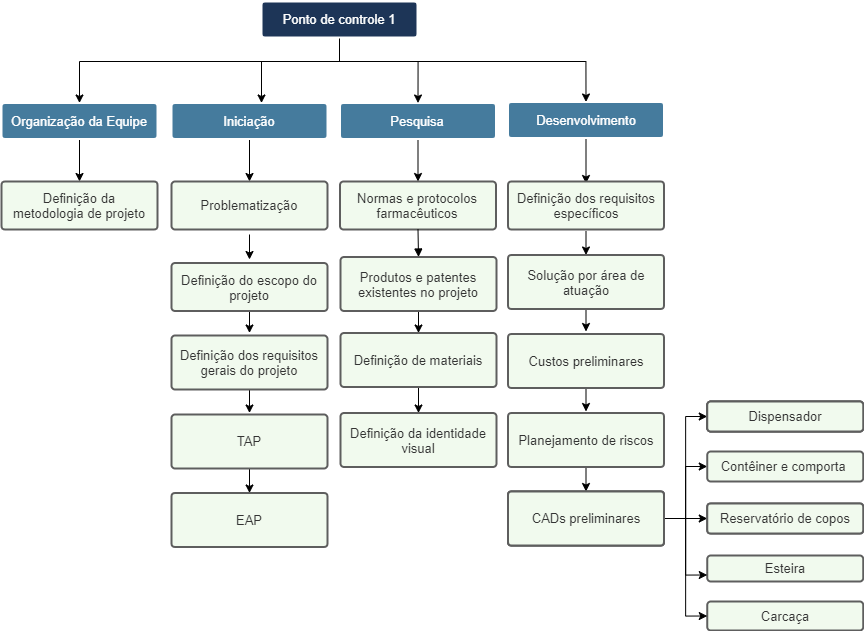
\includegraphics[width=\textwidth]{figuras/eap_pc1.png}
    \caption{Estrutura Analítica do Projeto PillWatcher - Ponto de Controle 1 }
    \label{fig:eap_pc1}
\end{figure}

\begin{landscape}
\begin{figure}[H]
    \centering
    \vspace{1cm}
    \hspace{-1cm}
    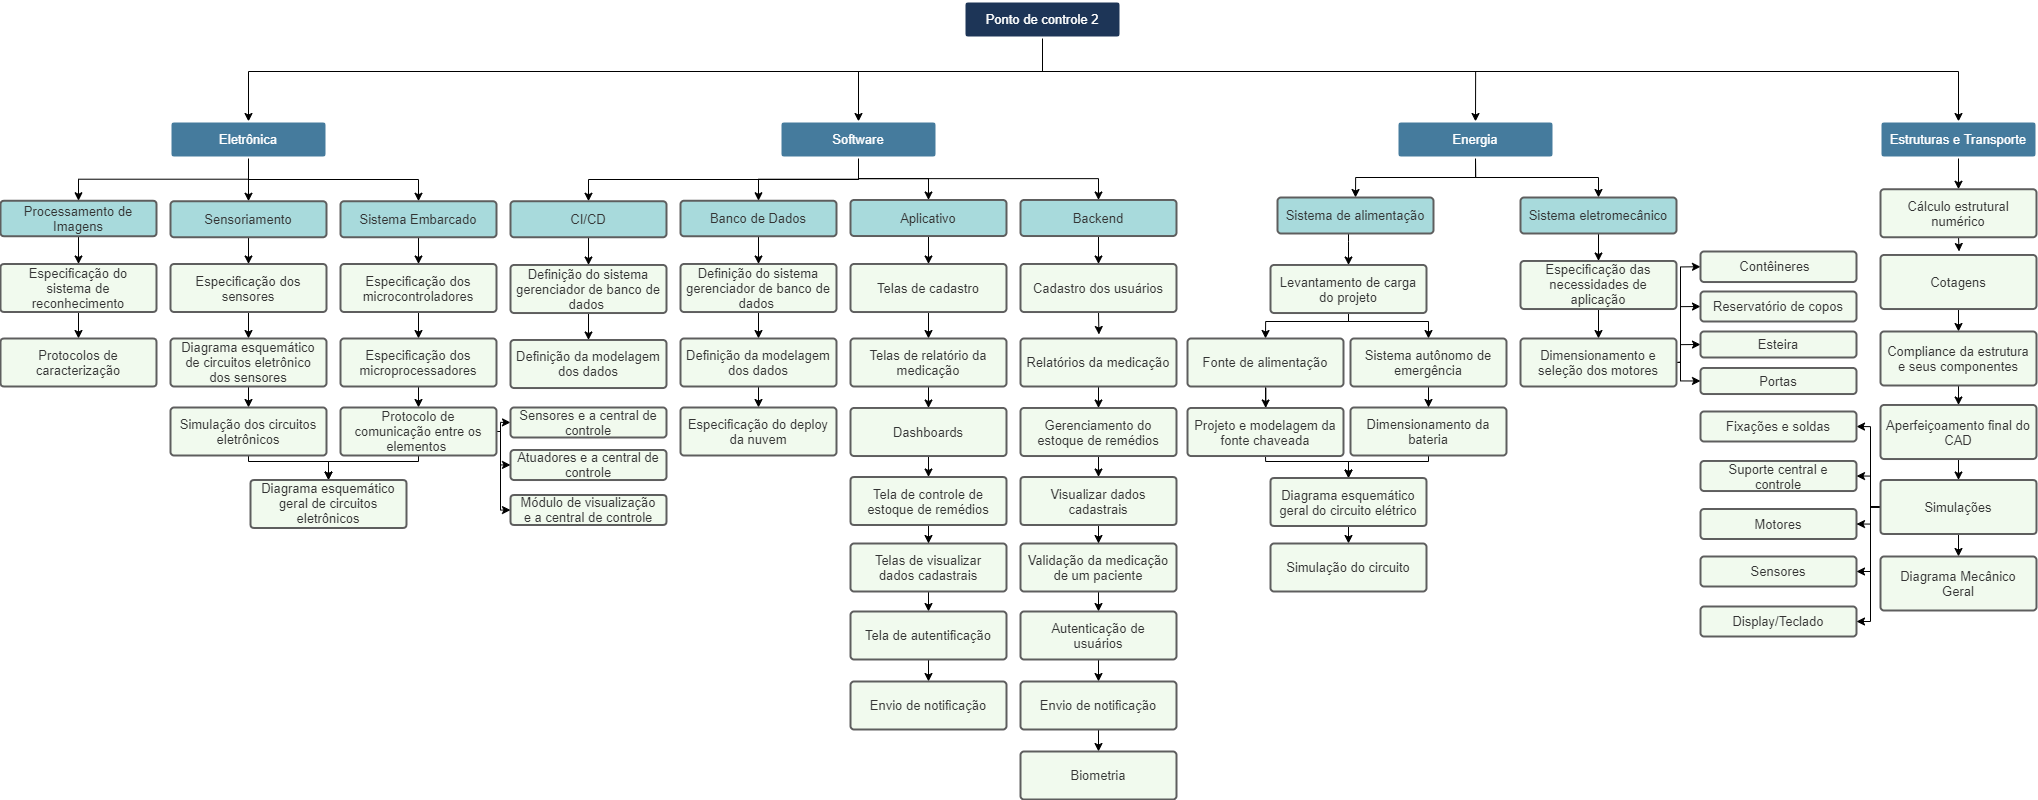
\includegraphics[scale=0.3]{figuras/eap_pc2.png}
    \caption{Estrutura Analítica do Projeto PillWatcher - Ponto de Controle 2 }
    \vspace{-5pt}
    \label{fig:eap_pc2}
\end{figure}
\end{landscape}

\begin{figure}[H]
    \centering
    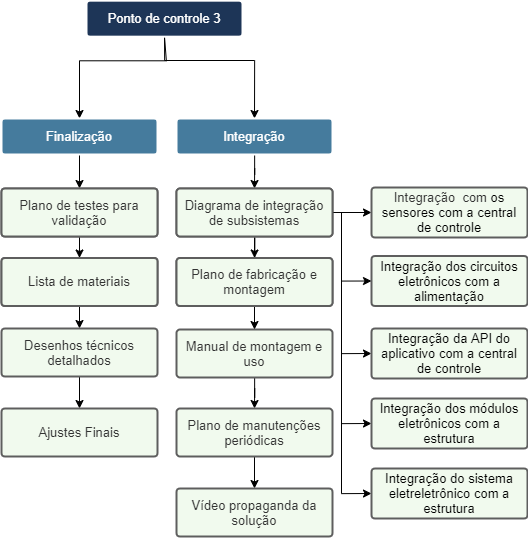
\includegraphics[width=0.7\textwidth]{figuras/eap_pc3.png}
    \caption{Estrutura Analítica do Projeto PillWatcher - Ponto de Controle 3 }
    \label{fig:eap_pc3}
\end{figure}

\begin{landscape}
\section{Estrutura Analítica Geral}
\begin{figure}[!htb]
    \centering
    \vspace{2cm}
    \hspace{-2cm}
    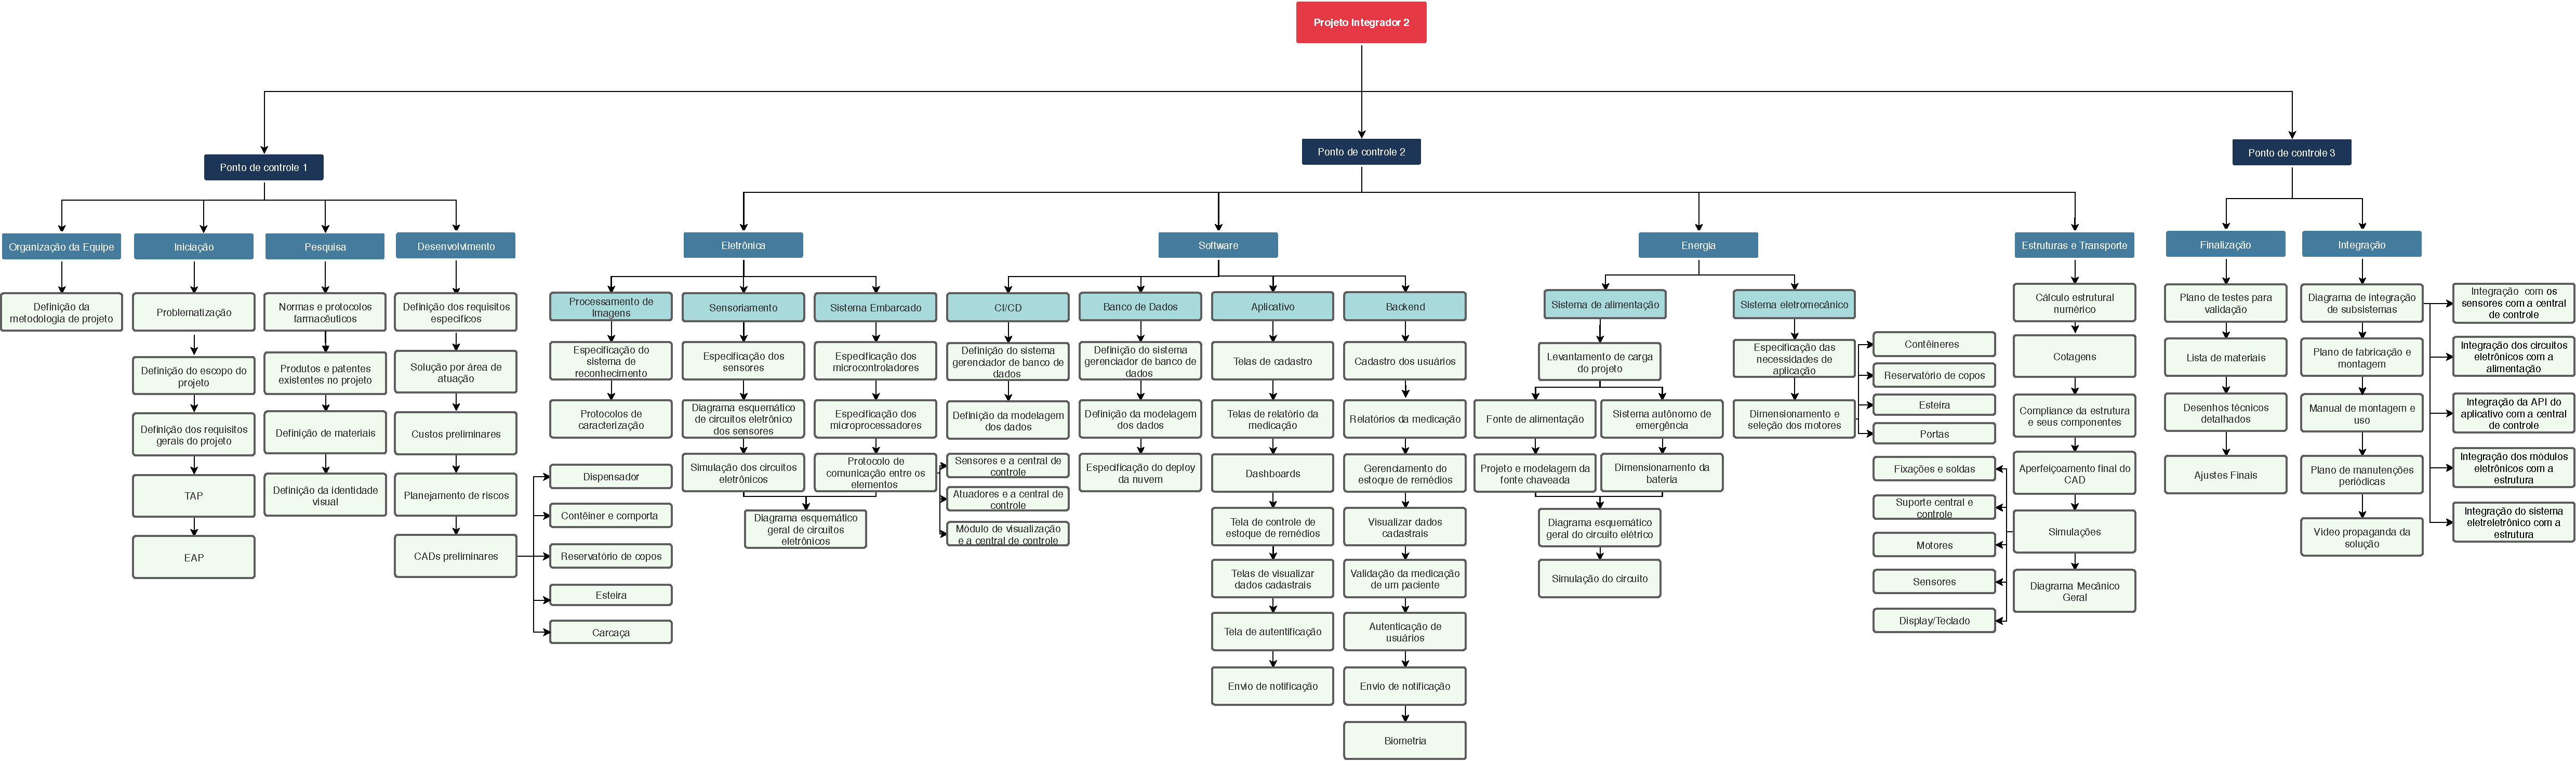
\includegraphics[width=1.55\textwidth, height=2\textheight,keepaspectratio]{figuras/EAP.pdf}
    \vspace{-5pt}
    \caption{Estrutura Analítica do Projeto PillWatcher}
\end{figure}
\end{landscape}
%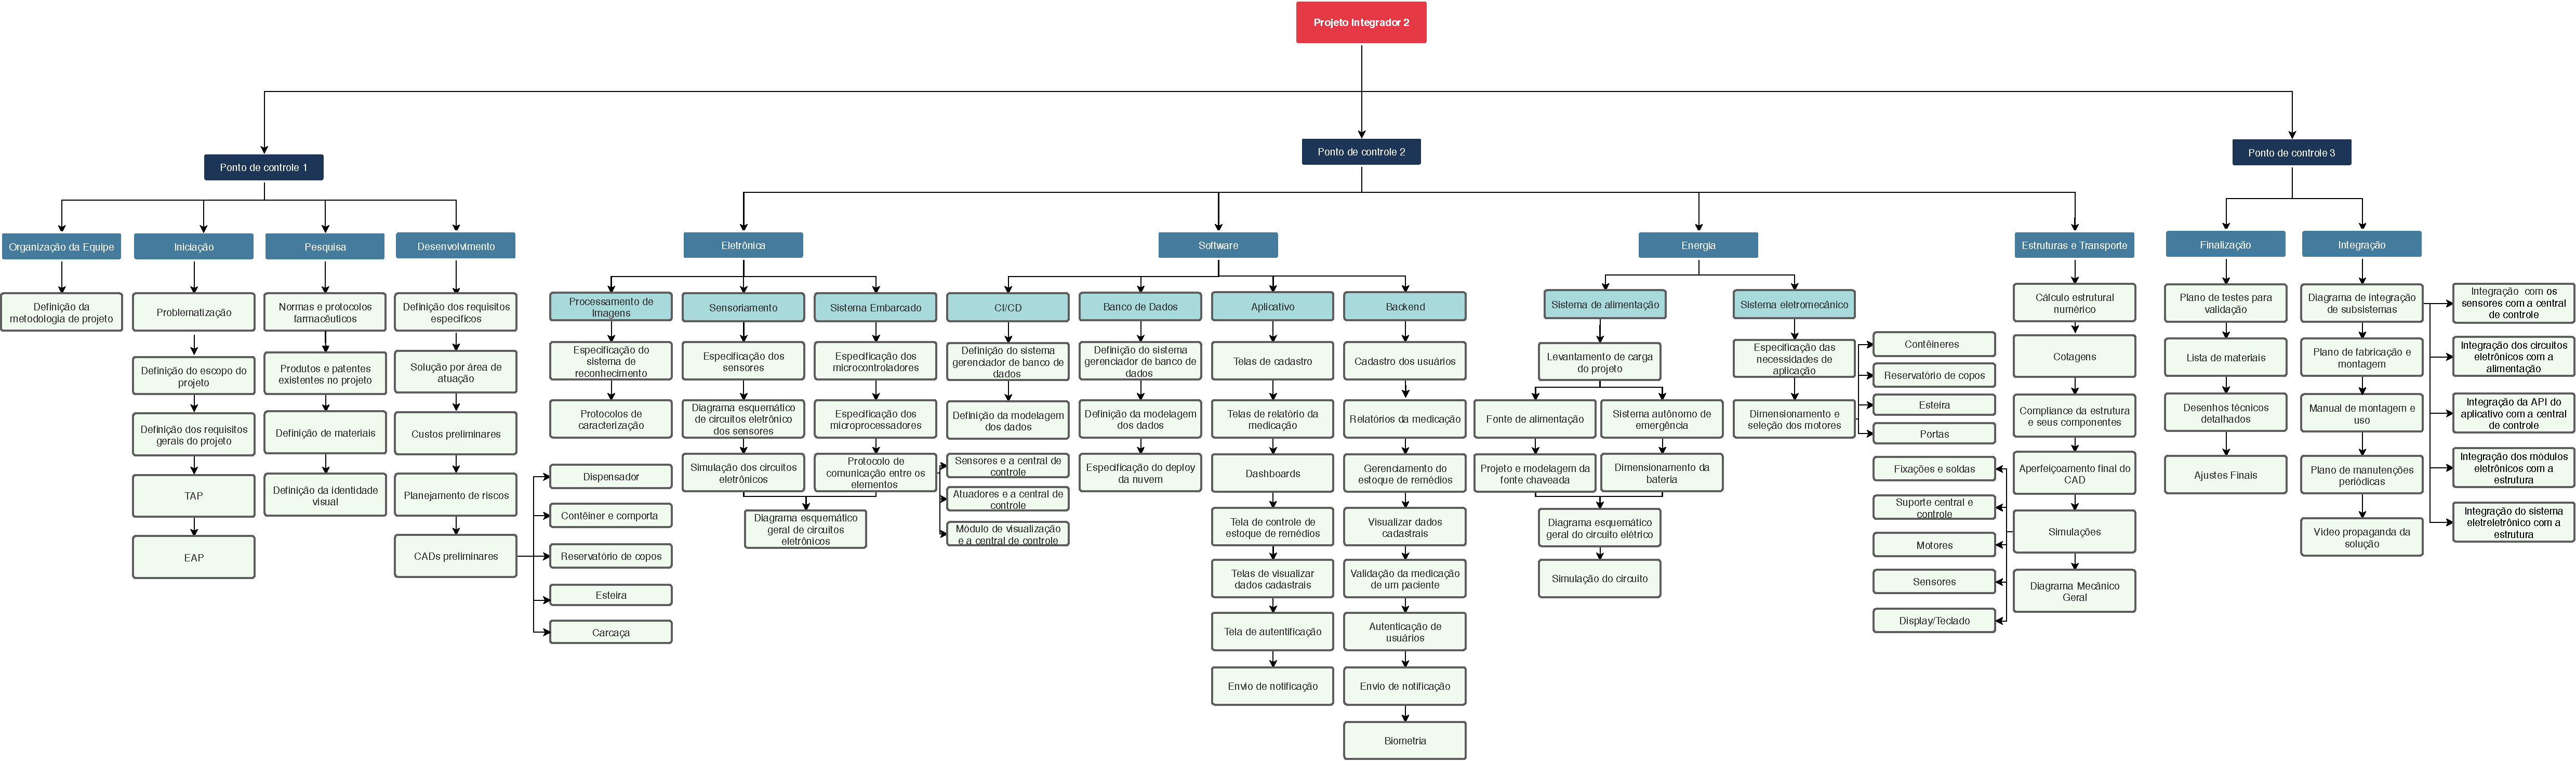
\includepdf[scale=0.73,angle=90,pages=1,pagecommand=\label{EAp}, offset=1cm -1.5cm]{figuras/EAP.pdf}

\chapter{Lista É/ Não É}
\label{Lista_app}

\begin{table}[H]
    \centering
    \caption{Lista É/Não é}
    \label{tab:lista_e_n_e}
    \begin{tabularx}{\textwidth}{|X|X|}
        \hline
        \rowcolor[HTML]{A8DADC}
        \multicolumn{1}{|X}{\textbf{É}} & \multicolumn{1}{|X|}{\textbf{Não é}} \\ 
        \hline
        1.1 É um sistema automático & 1.2 Não é um sistema autônomo \\ 
        \hline
        2.1 É um dispensador de medicamentos sólidos (comprimidos, drágeas e capsulas) & 2.2 Não é um dispensador de medicamentos líquidos, invetáveis ou pastosos \\ 
        \hline
        3.1 A quantidade de contêineres é pré-definida & 3.2 A quantidade de contêineres não é variável\\ 
        \hline
        4.1 Os contêineres recebem separadamente cada medicamento & 4.2 Os contêineres não armazenam doses de diferentes medicamentos \\
        \hline
        5.1 É um dispositivo que funciona interligado à rede elétrica & 5.2 Não é um dispositivo que deve funcionar desconectado da rede, salvo em falha da fonte primária \\ 
        \hline
        6.1 Para uso coletivo & 6.2 Para uso individual\\ 
        \hline
        7.1 Controlado via aplicativo & 7.2 Controlado manualmente via dispensador\\ 
        \hline
        8.1 Responsável por verificar se a medicação foi corretamente armazenada e separada em doses & 8.2 Responsável por ministrar a medicação\\ 
        \hline
        9.1 É um dispositivo fixo & 9.2 Não é um dispositivo transportável \\ 
        \hline
    \end{tabularx}
\end{table}


\chapter{Cronograma}\label{roadmap}

\vspace{-1.6cm}
\begin{figure}[H]
    \centering
    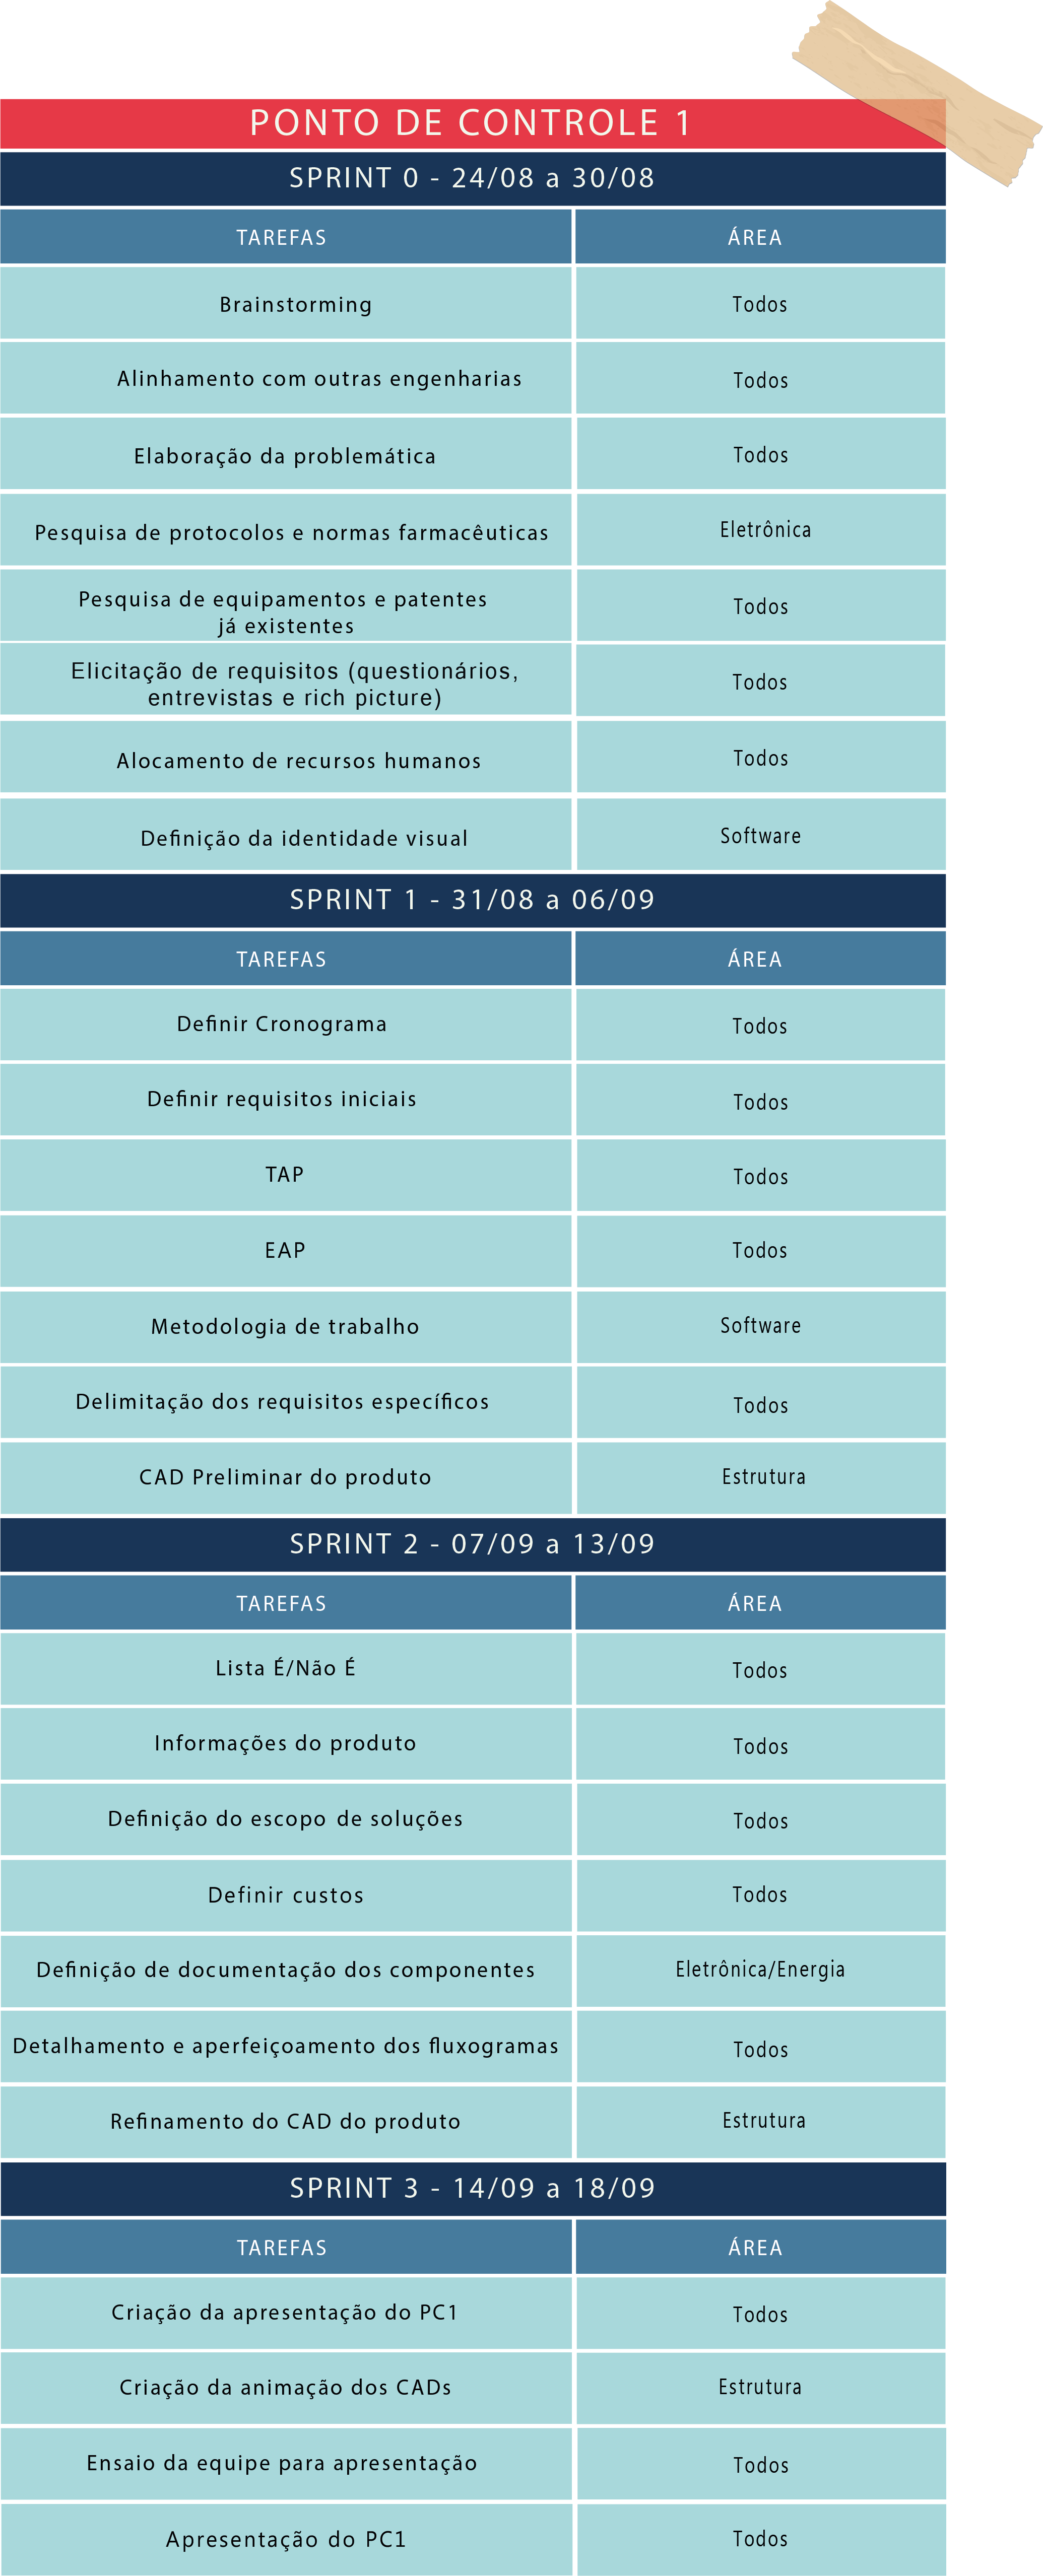
\includegraphics[width=0.5\textwidth]{figuras/sprint-pc1.png}
    \caption{Planejamento Ponto de Controle 1}
    \label{fig:Sprint_pc1}
\end{figure}

\begin{figure}[H]
    \centering
    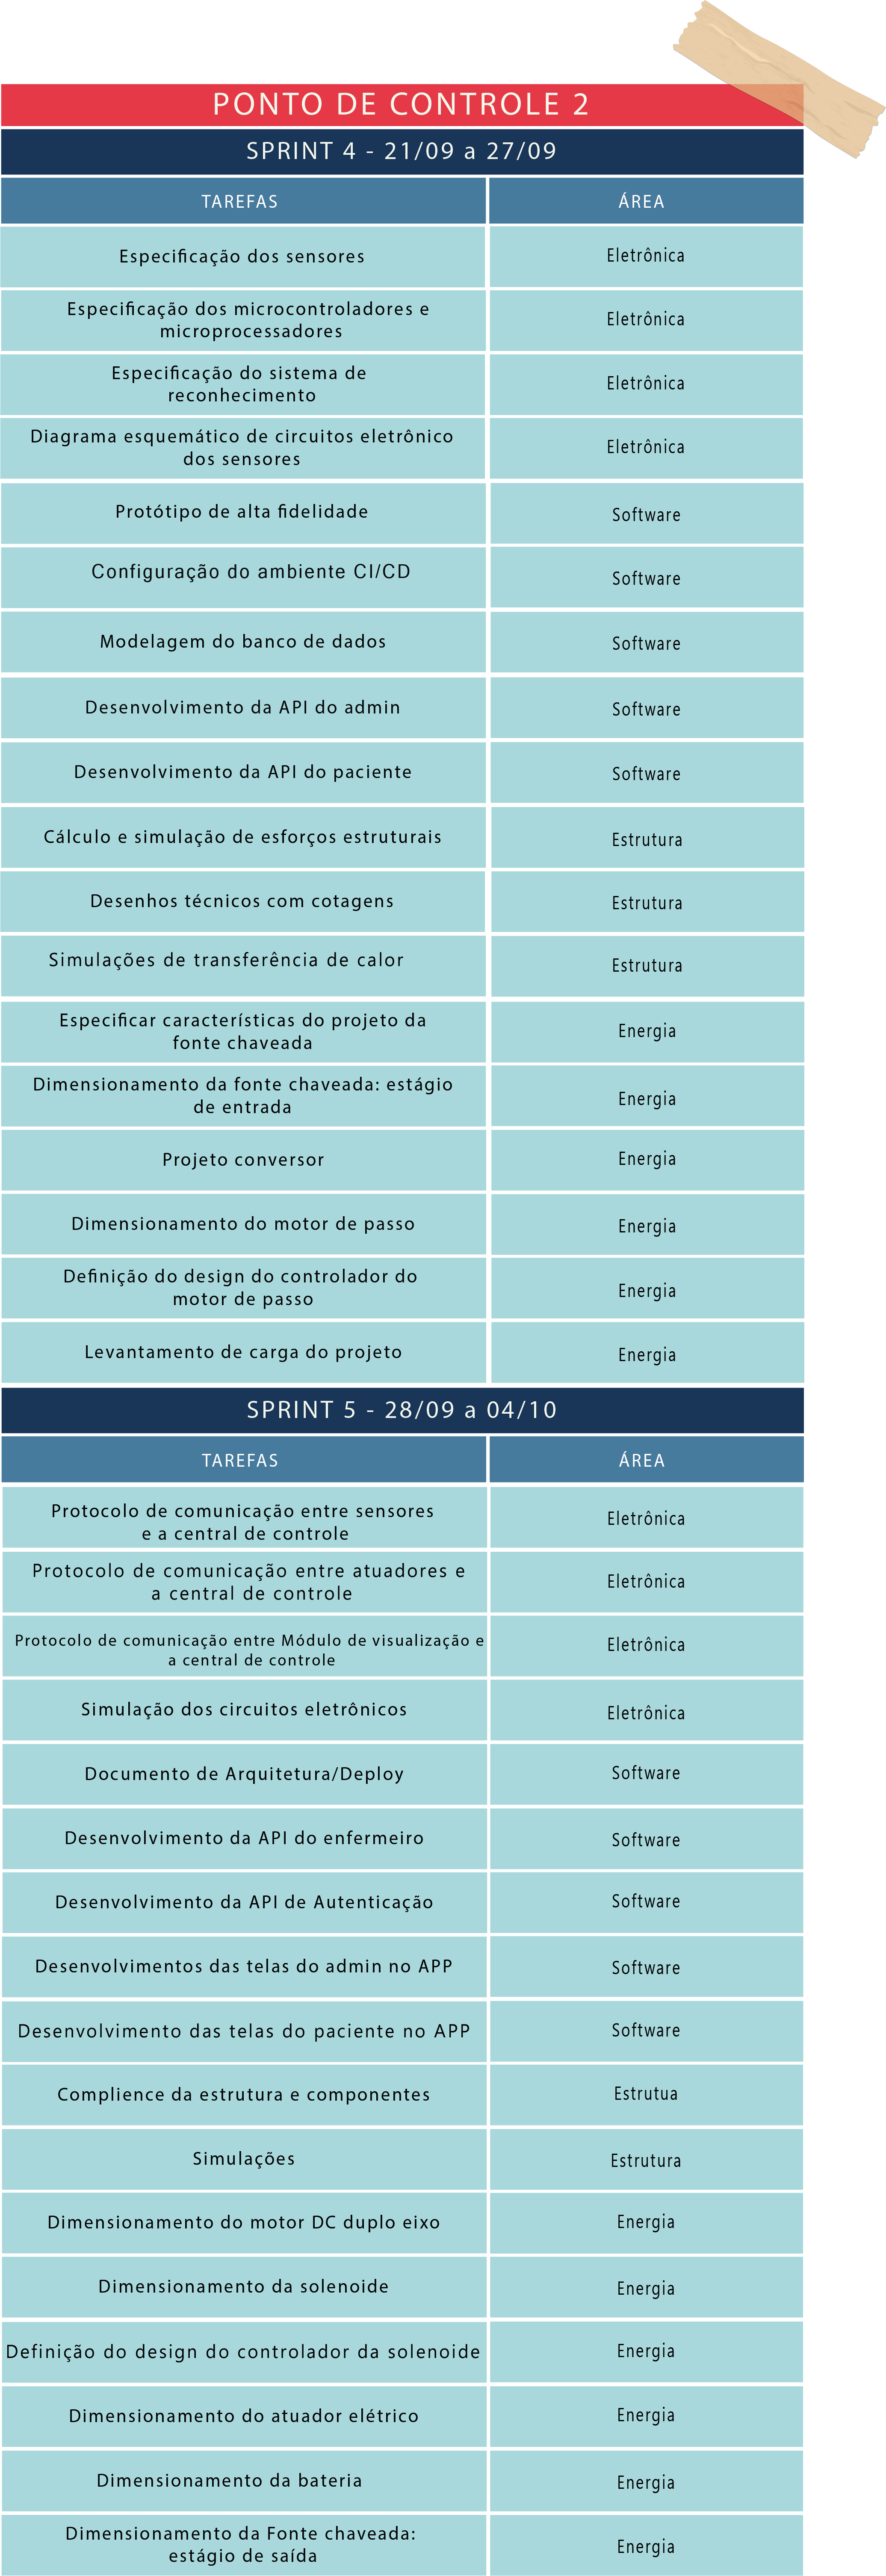
\includegraphics[width=0.5\textwidth]{figuras/sprint-pc2-1.png}
    \caption{Planejamento Ponto de Controle 2}
    \label{fig:Sprint_pc2}
\end{figure}

\begin{figure}[H]
    \centering
    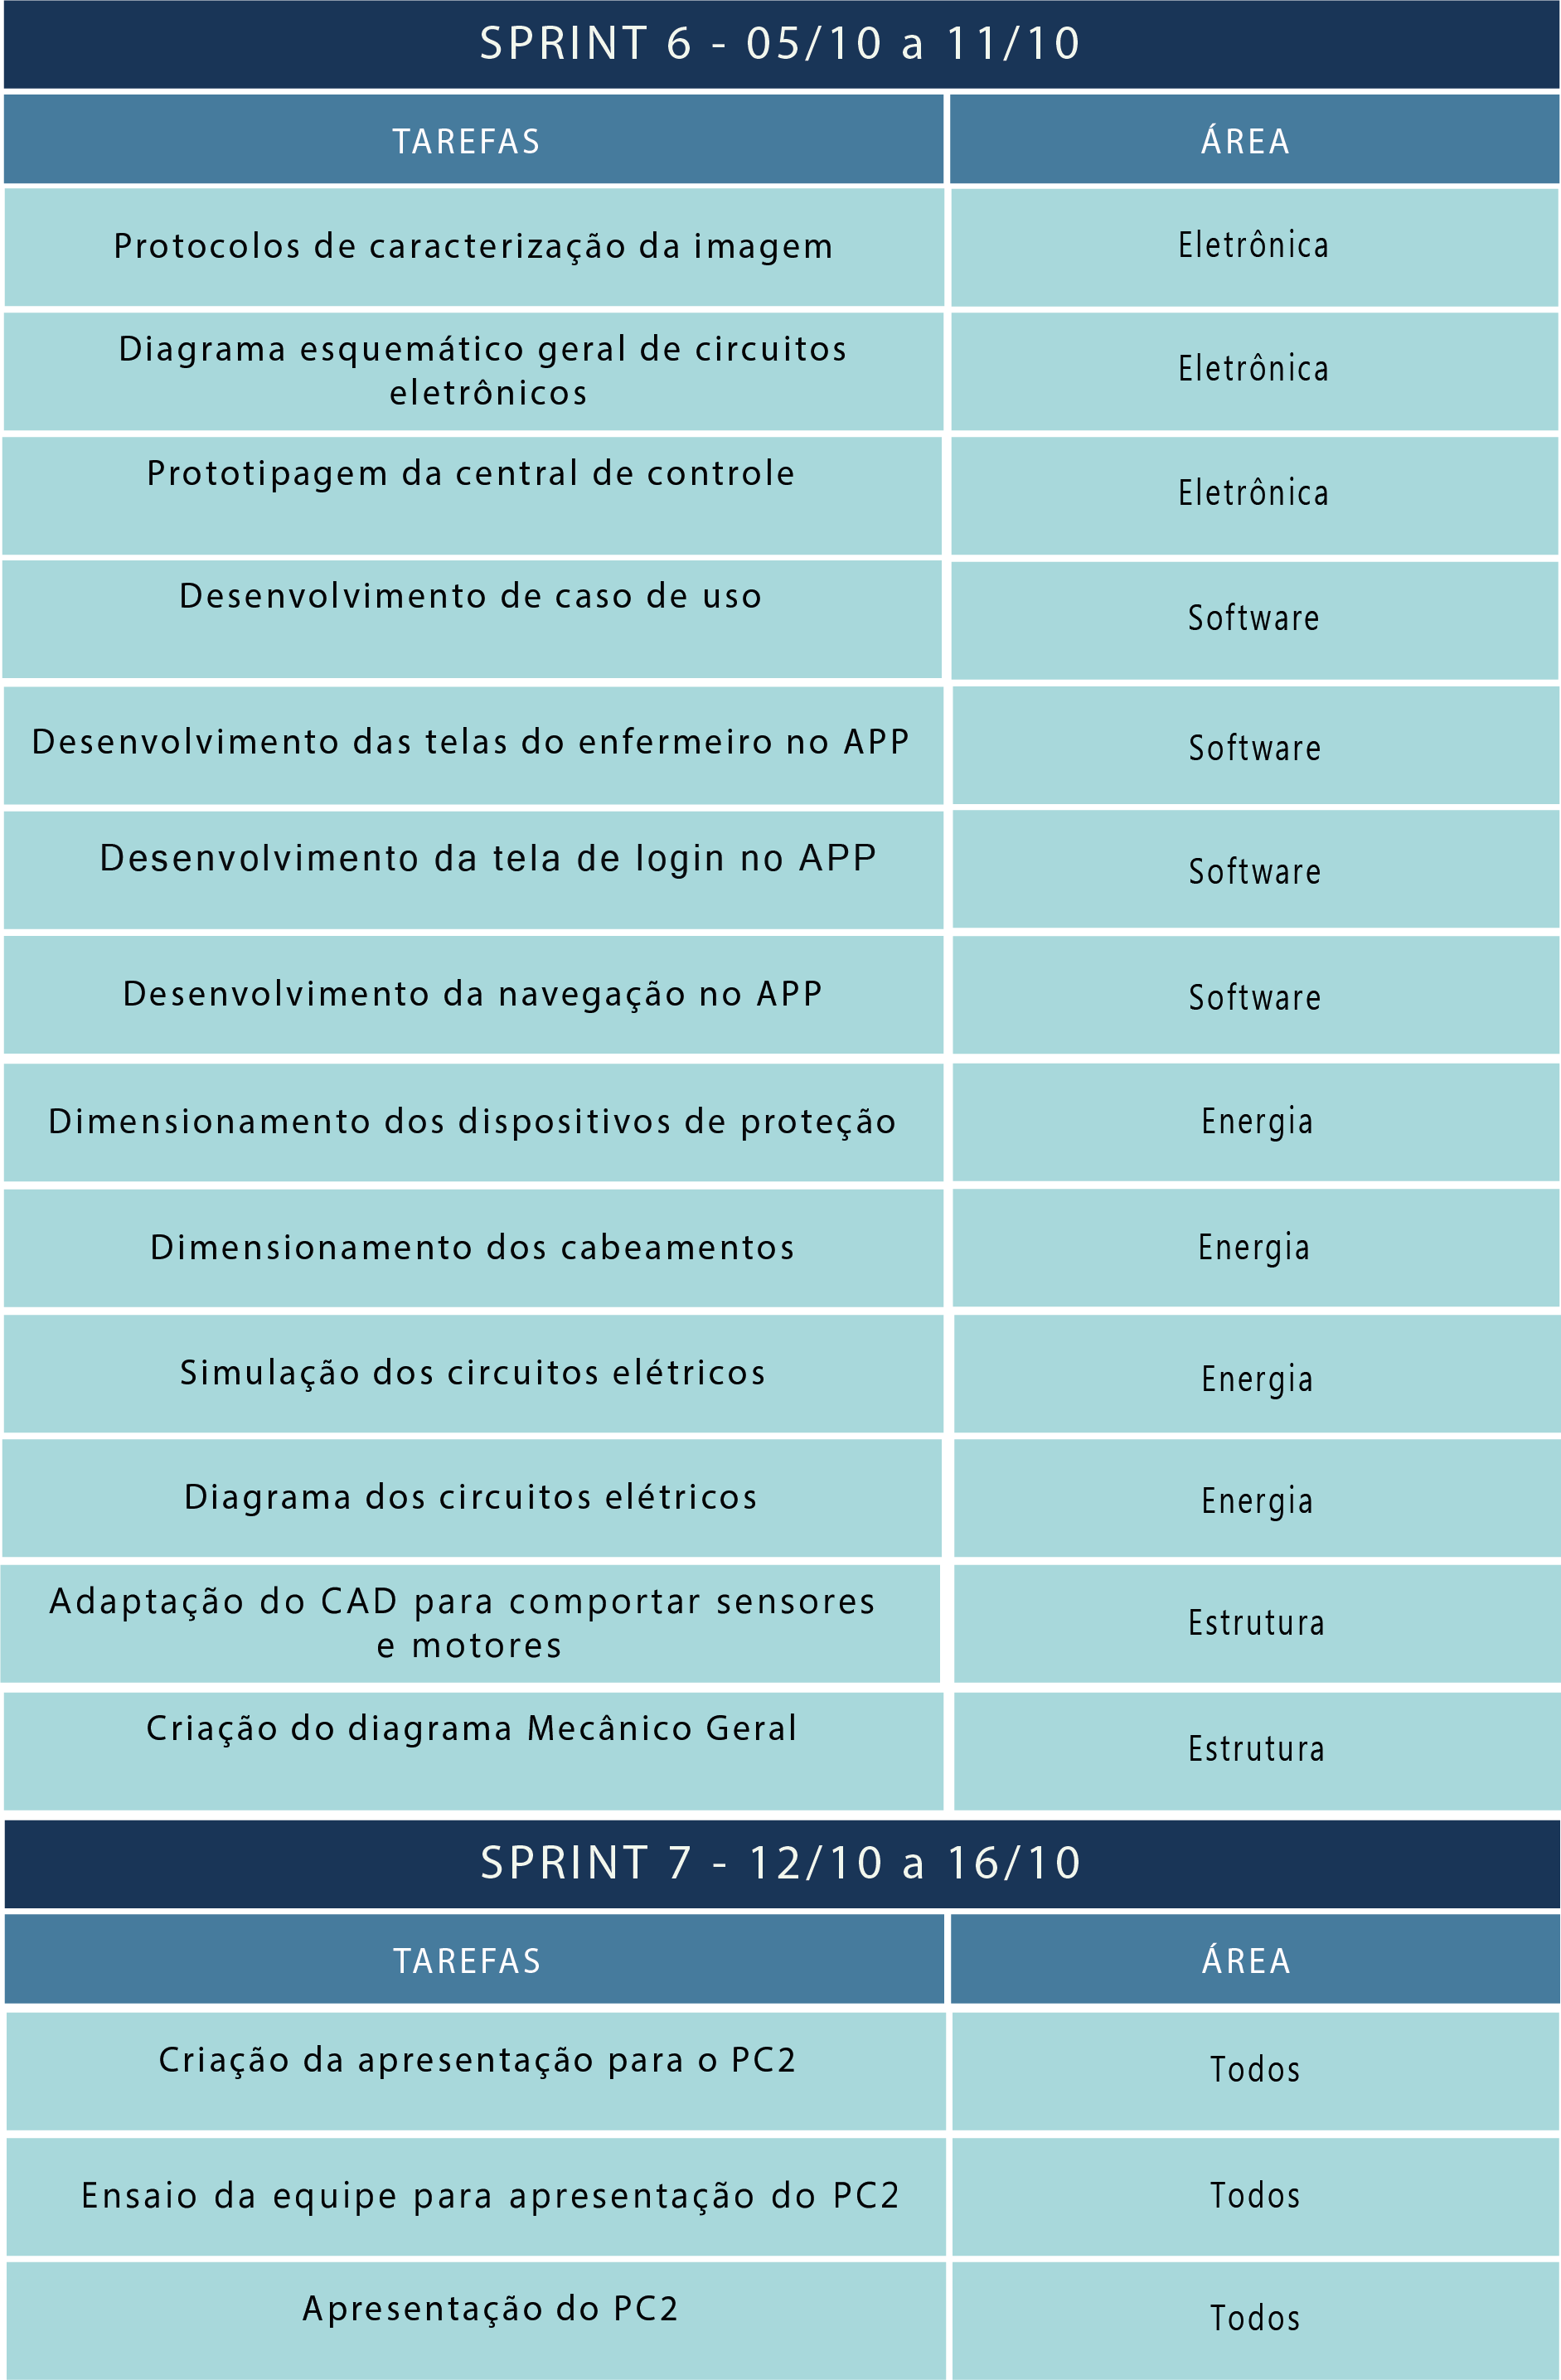
\includegraphics[width=0.5\textwidth]{figuras/sprint-pc2-2.png}
    \caption{Planejamento Ponto de Controle 2}
    \label{fig:Sprint_pc2_1}
\end{figure}

\begin{figure}[H]
    \centering
    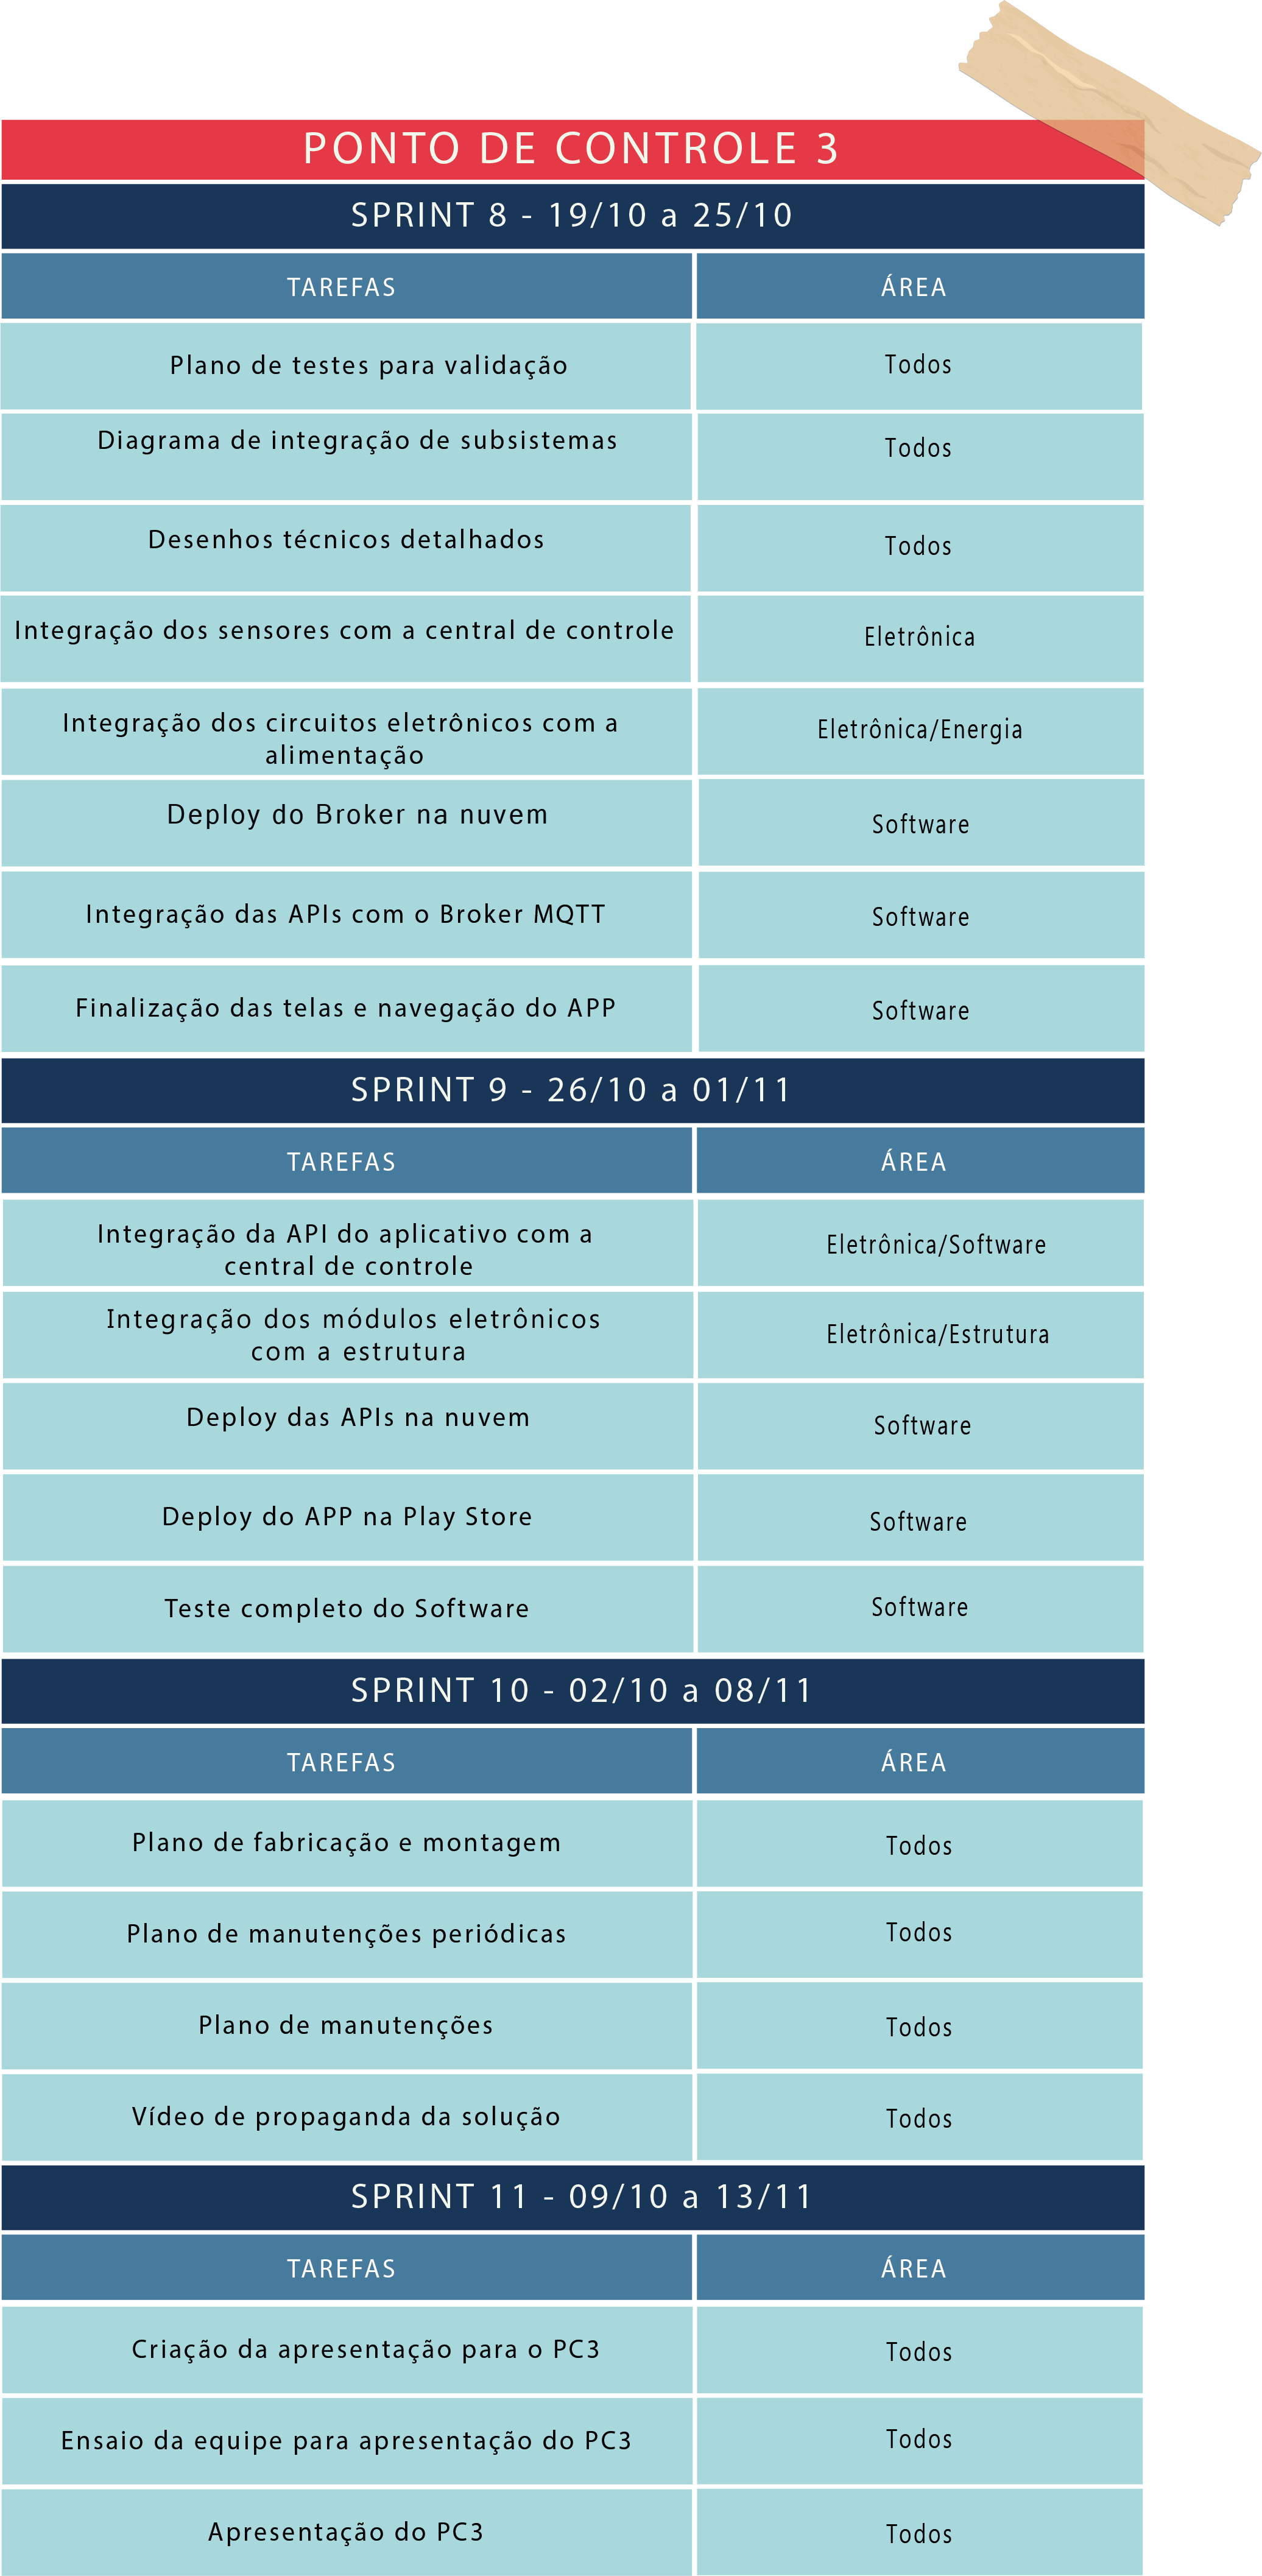
\includegraphics[width=0.5\textwidth]{figuras/sprint-pc3.png}
    \caption{Planejamento Ponto de Controle 3}
    \label{fig:Sprint_pc3}
\end{figure}

% CADs Preliminares
\chapter{Desenhos Técnicos Preliminares}\label{cad_preliminar}

\vspace{3cm}

\begin{figure}[H]
    \centering
    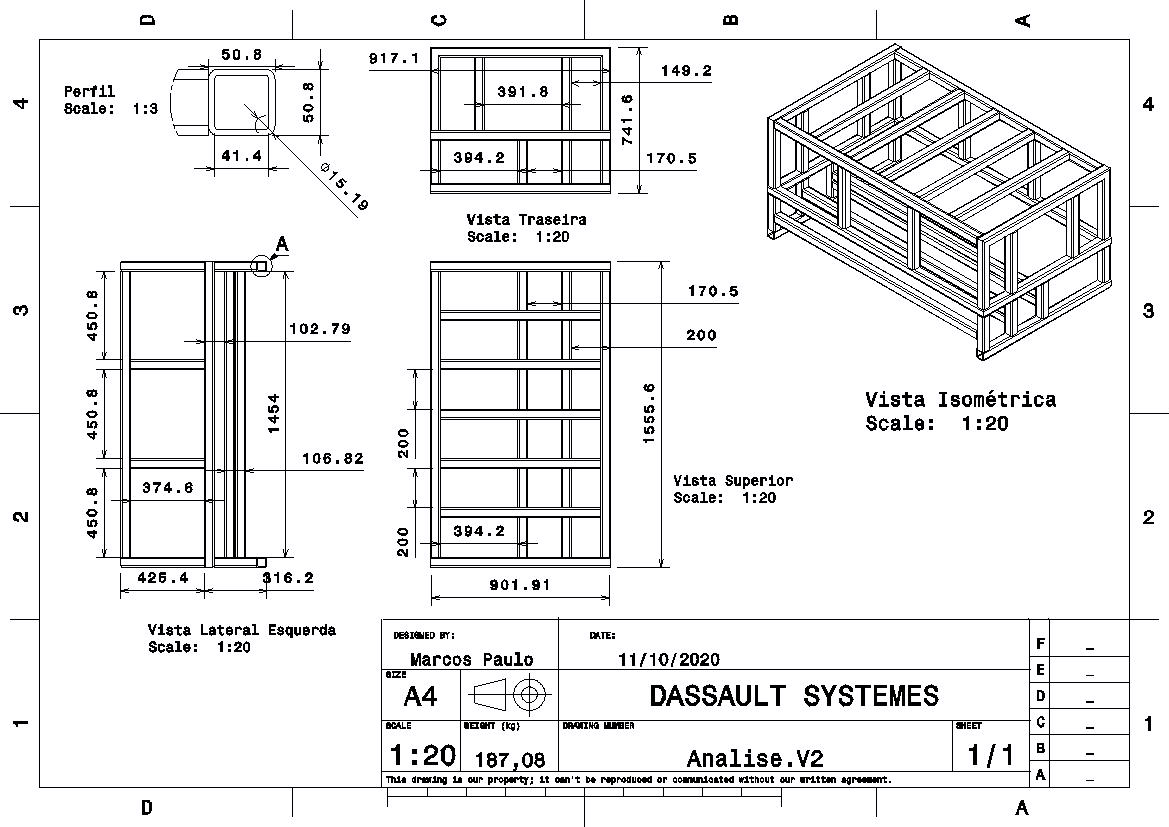
\includegraphics[width=1\textwidth]{figuras/estrutura/Desenhos/Estrutura_Tubular.jpg}
    \caption{Desenho técnico da Estrutura Tubular (\ref{retorno_tubos_perfilquadrado})}
    \label{fig:estruturatubular}
\end{figure}

\begin{figure}[H]
    \centering
    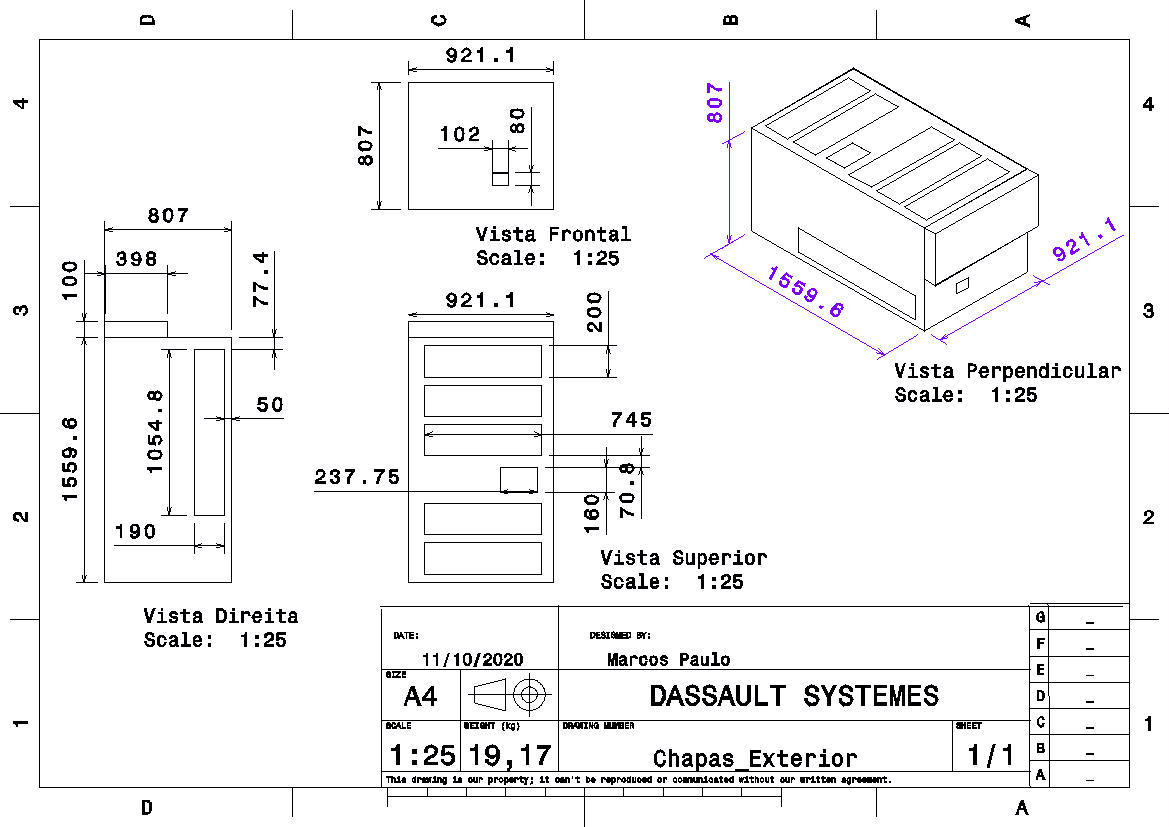
\includegraphics[width=0.9\textwidth]{figuras/estrutura/Desenhos/Chapas_Exterior.jpg}
    \caption{Desenho técnico das Chapas da Carcaça (\ref{retorno_chapas})}
    \label{fig:chapasexterior}
\end{figure}

\begin{figure}[H]
    \centering
    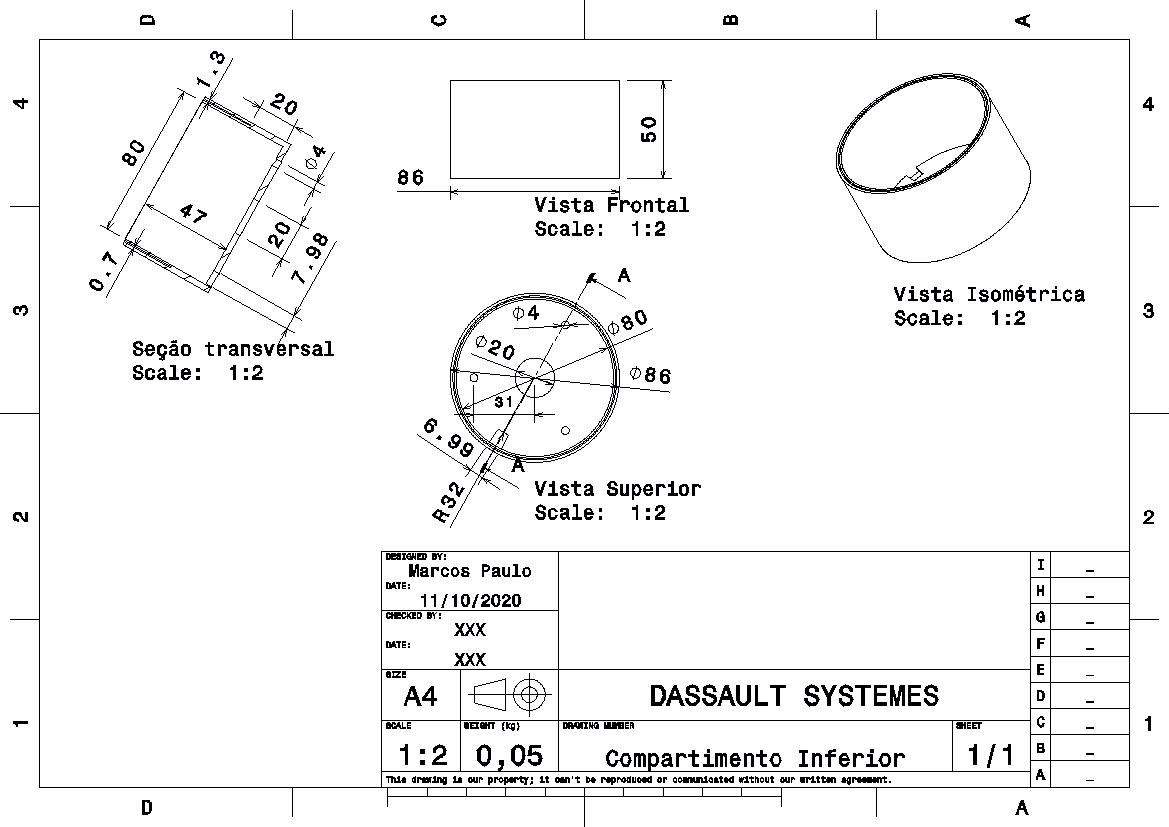
\includegraphics[width=0.9\textwidth]{figuras/estrutura/Desenhos/Compartimento_Inferior.jpg}
    \caption{Desenho técnico do Compartimento Inferior do Contêiner (\ref{retorno_compartimentoinferior})}
    \label{fig:compartimentoinferior}
\end{figure}

\begin{figure}[H]
    \centering
    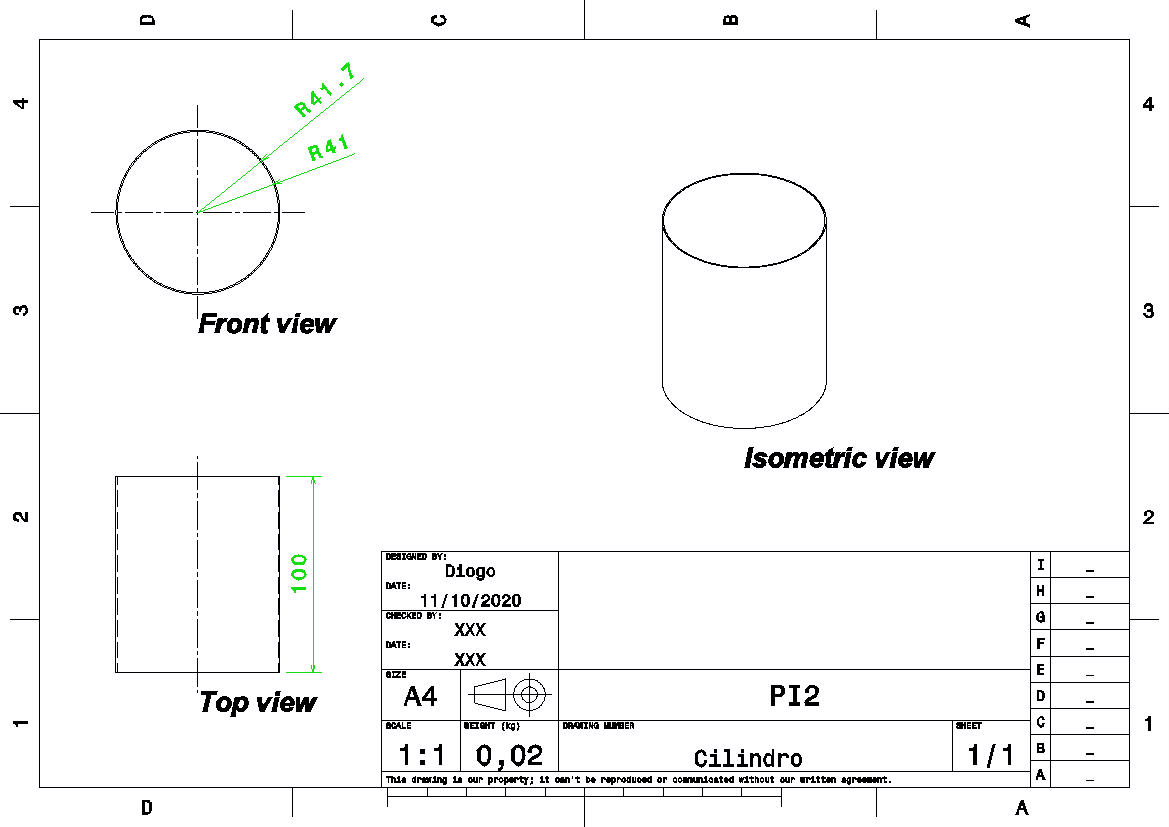
\includegraphics[width=0.9\textwidth]{figuras/estrutura/Desenhos/Drawing1_Cilindro.jpg}
    \caption{Desenho técnico do cilindro do contêiner (\ref{retorno_cilindro})}
    \label{fig:cilindro}
\end{figure}

\begin{figure}[H]
    \centering
    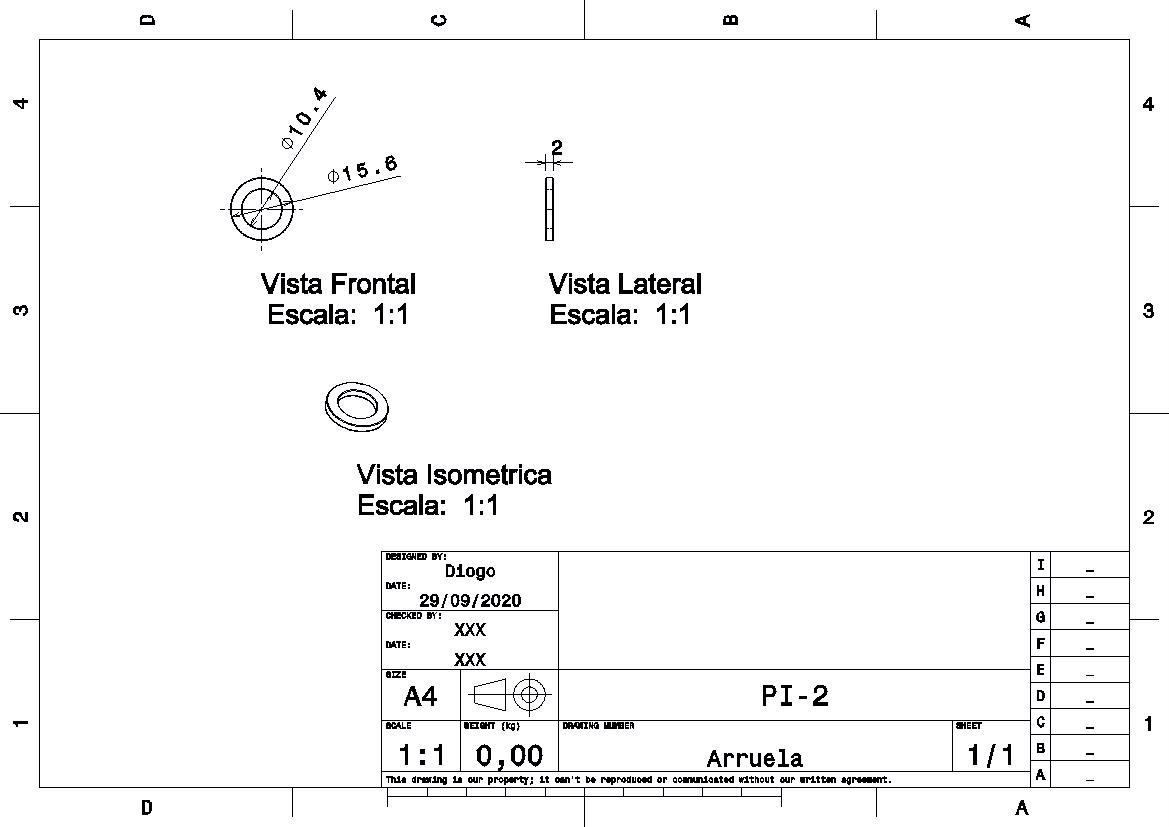
\includegraphics[width=0.9\textwidth]{figuras/estrutura/Desenhos/Drawing1_Arruela.jpg}
    \caption{Desenho técnico da arruela do contêiner (\ref{retorno_engrenagem_fundo})}
    \label{fig:arruela}
\end{figure}

\begin{figure}[H]
    \centering
    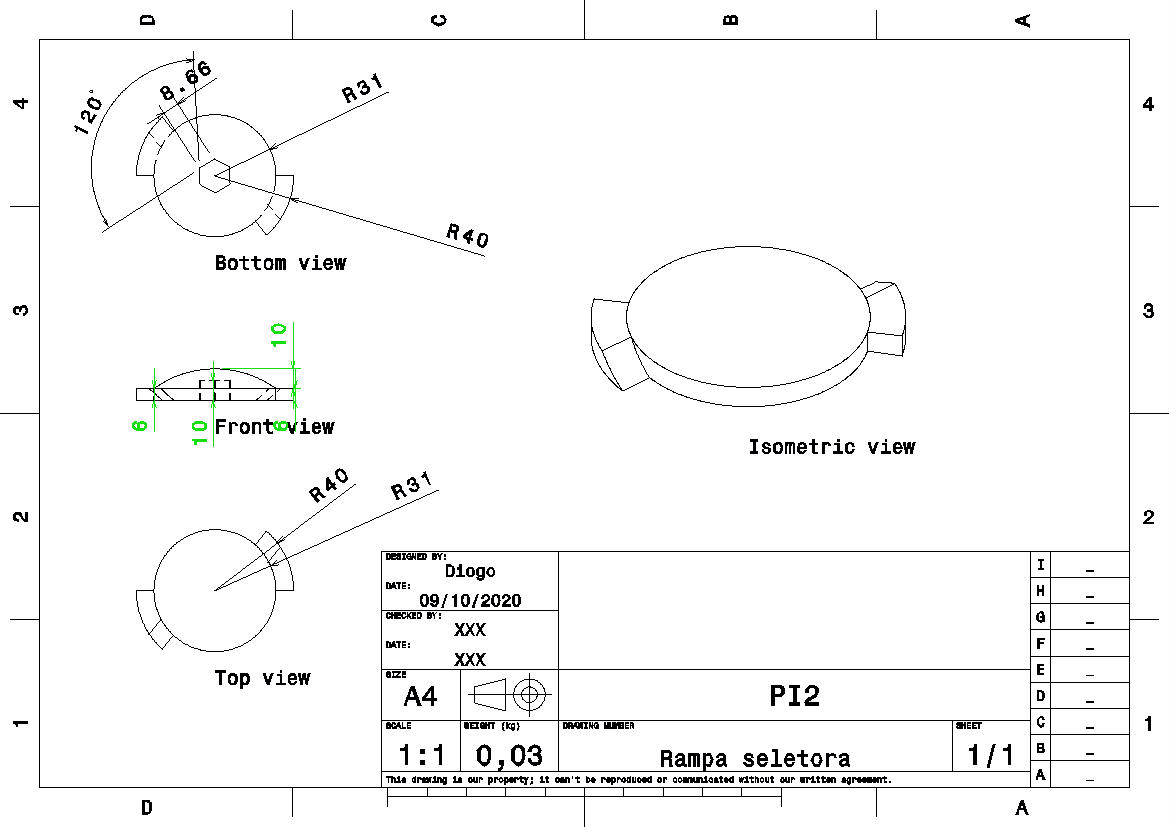
\includegraphics[width=0.9\textwidth]{figuras/estrutura/Desenhos/Drawing1_RampaSeletora.jpg}
    \caption{Desenho técnico das rampa seletora do contêiner (\ref{retorno_rampaseletora})}
    \label{fig:rampaseletora}
\end{figure}

\begin{figure}[H]
    \centering
    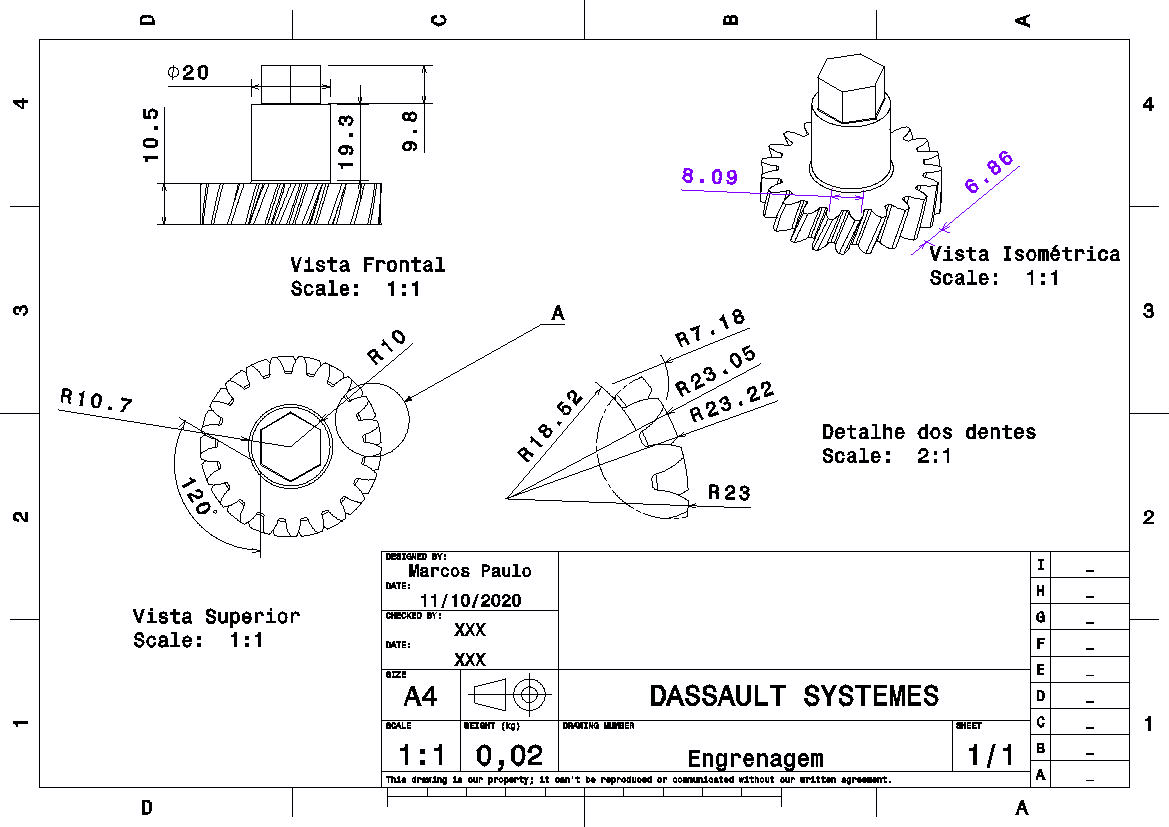
\includegraphics[width=0.9\textwidth]{figuras/estrutura/Desenhos/Engrenagem_Fundo.jpg}
    \caption{Desenho técnico da engrenagem do contêiner (\ref{retorno_engrenagem_fundo})}
    \label{fig:engrenagem_fundo}
\end{figure}


\begin{figure}[H]
    \centering
    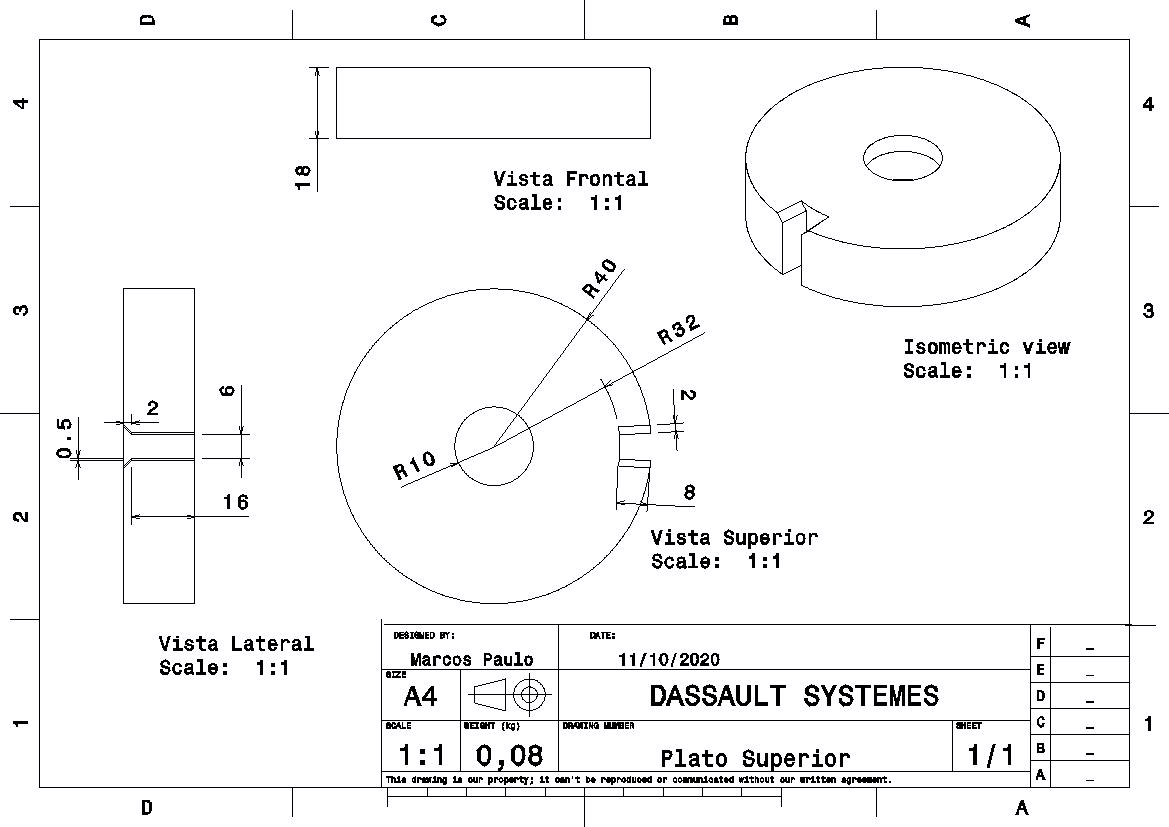
\includegraphics[width=0.9\textwidth]{figuras/estrutura/Desenhos/Plato_Superior.jpg}
    \caption{Desenho técnico do platô superior do contêiner (\ref{retorno_platosuperior})}
    \label{fig:platosuperior}
\end{figure}

\begin{figure}[H]
    \centering
    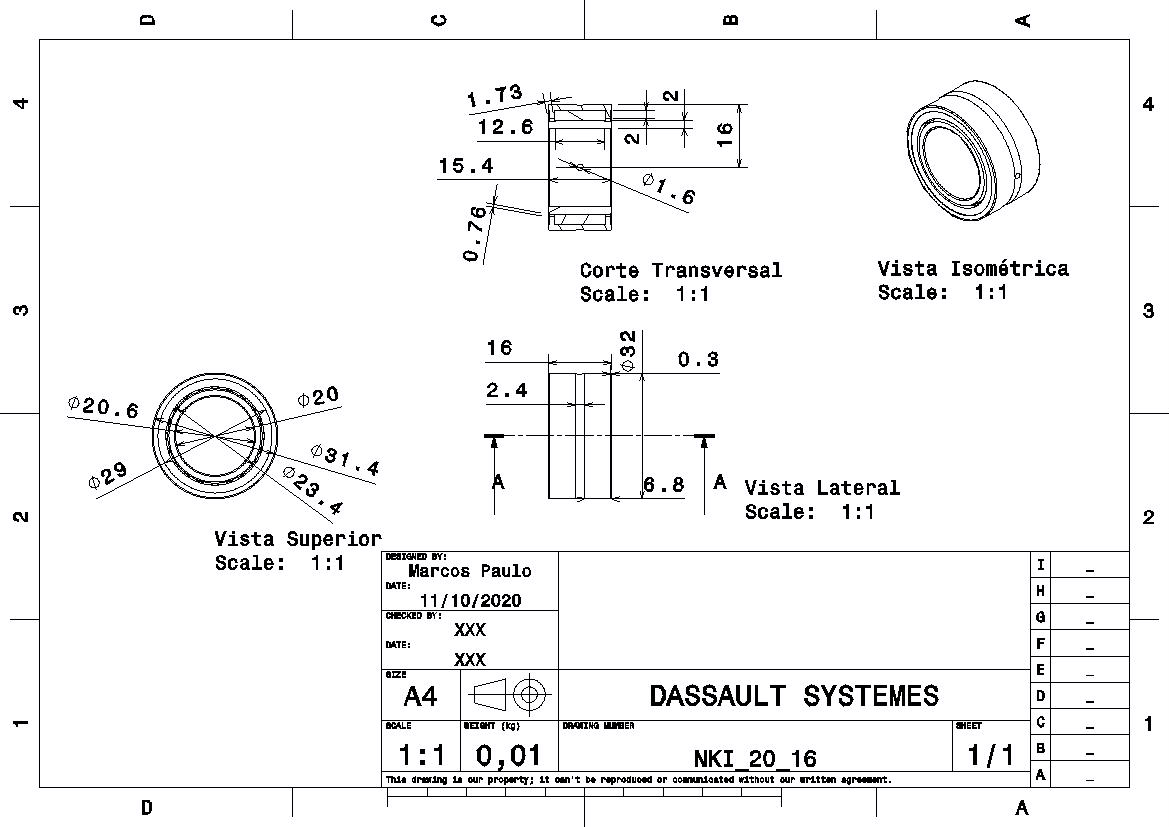
\includegraphics[width=0.9\textwidth]{figuras/estrutura/Desenhos/Rolamento_engrenagem.jpg}
    \caption{Desenho técnico do rolamento da engrenagem (\ref{retorno_engrenagem_fundo})}
    \label{fig:rolamento_engrenagem}
\end{figure}

\begin{figure}[H]
    \centering
    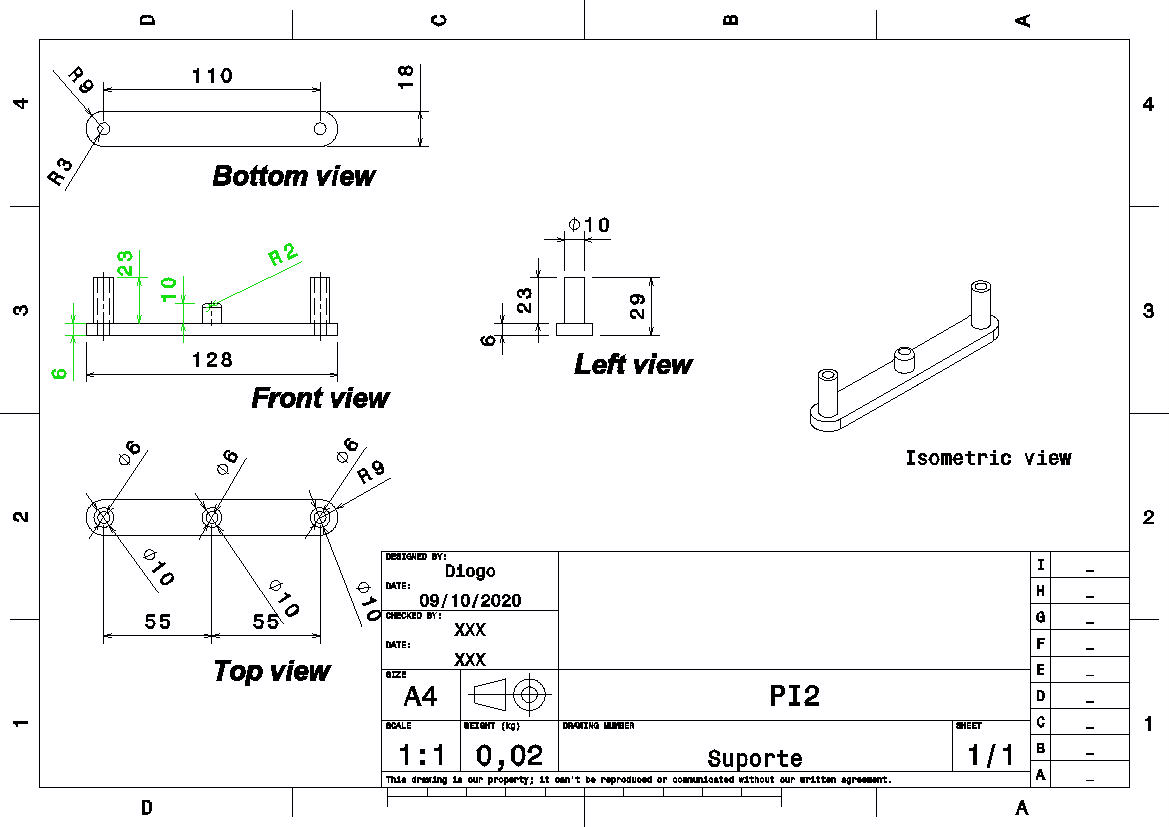
\includegraphics[width=0.9\textwidth]{figuras/estrutura/Desenhos/Suporte_Engrenagem_Container.jpg}
    \caption{Desenho técnico do suporte da engrenagem no contêiner (\ref{retorno_suporte_engrenagem})}
    \label{fig:supp_engrenagem}
\end{figure}

\begin{figure}[H]
    \centering
    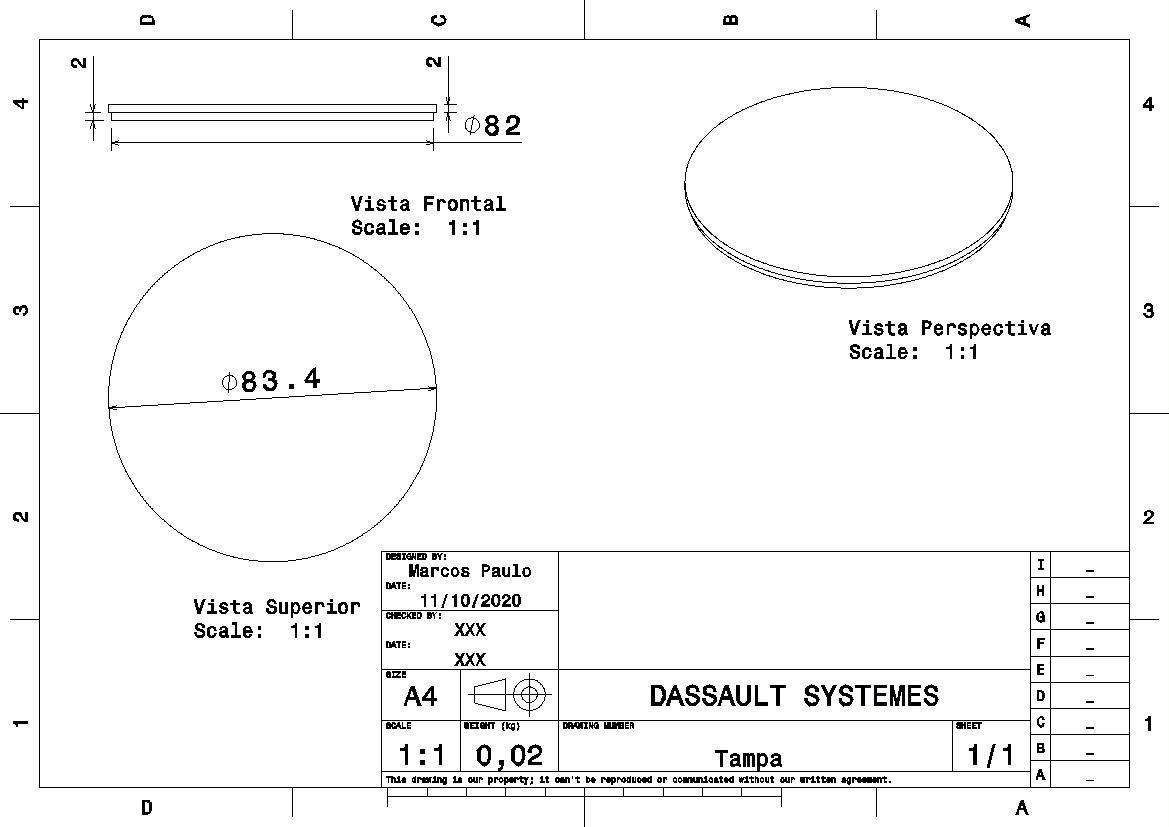
\includegraphics[width=0.9\textwidth]{figuras/estrutura/Desenhos/Tampa_Container.jpg}
    \caption{Desenho técnico da tampa do contêiner (\ref{retorno_tampa})}
    \label{fig:tampa}
\end{figure}

\begin{figure}[H]
    \centering
    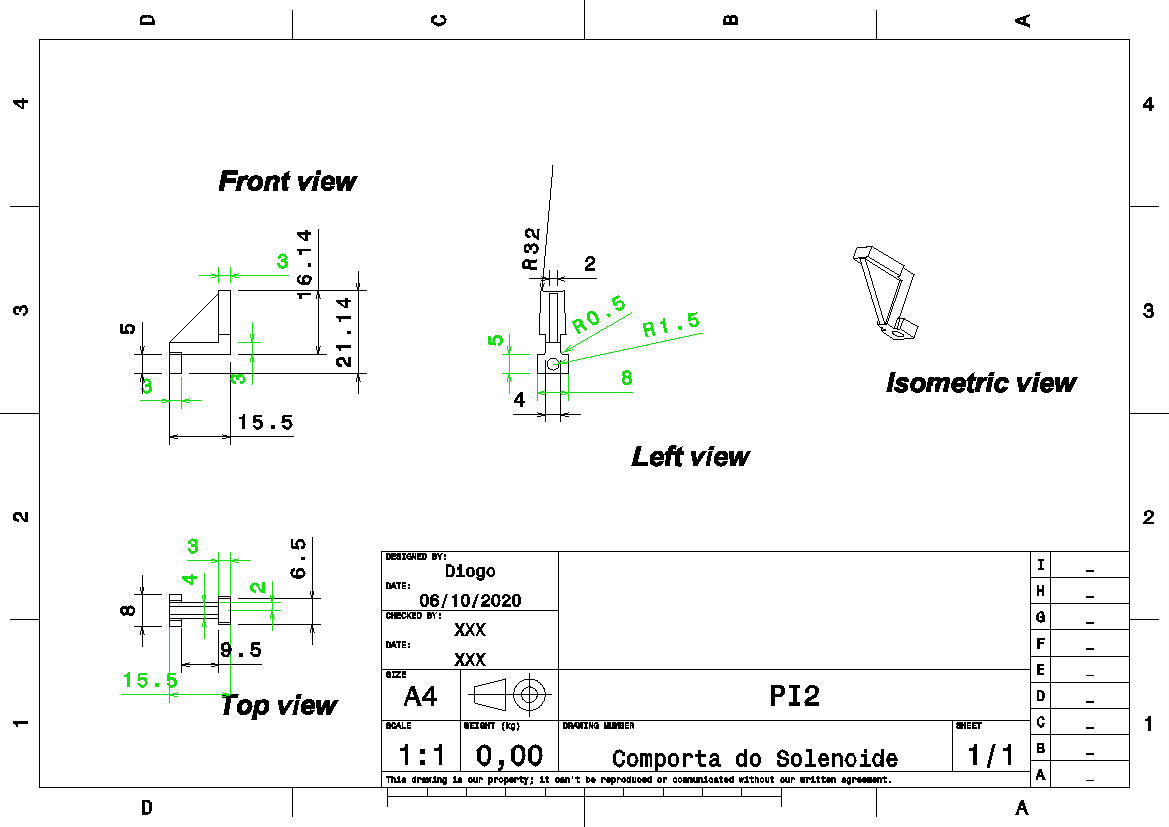
\includegraphics[width=0.9\textwidth]{figuras/estrutura/Desenhos/Drawing1_Comporta_do_Solenoide.jpg}
    \caption{Desenho técnico da comporta do contêiner (\ref{retorno_comporta})}
    \label{fig:comporta}
\end{figure}

\begin{figure}[H]
    \centering
    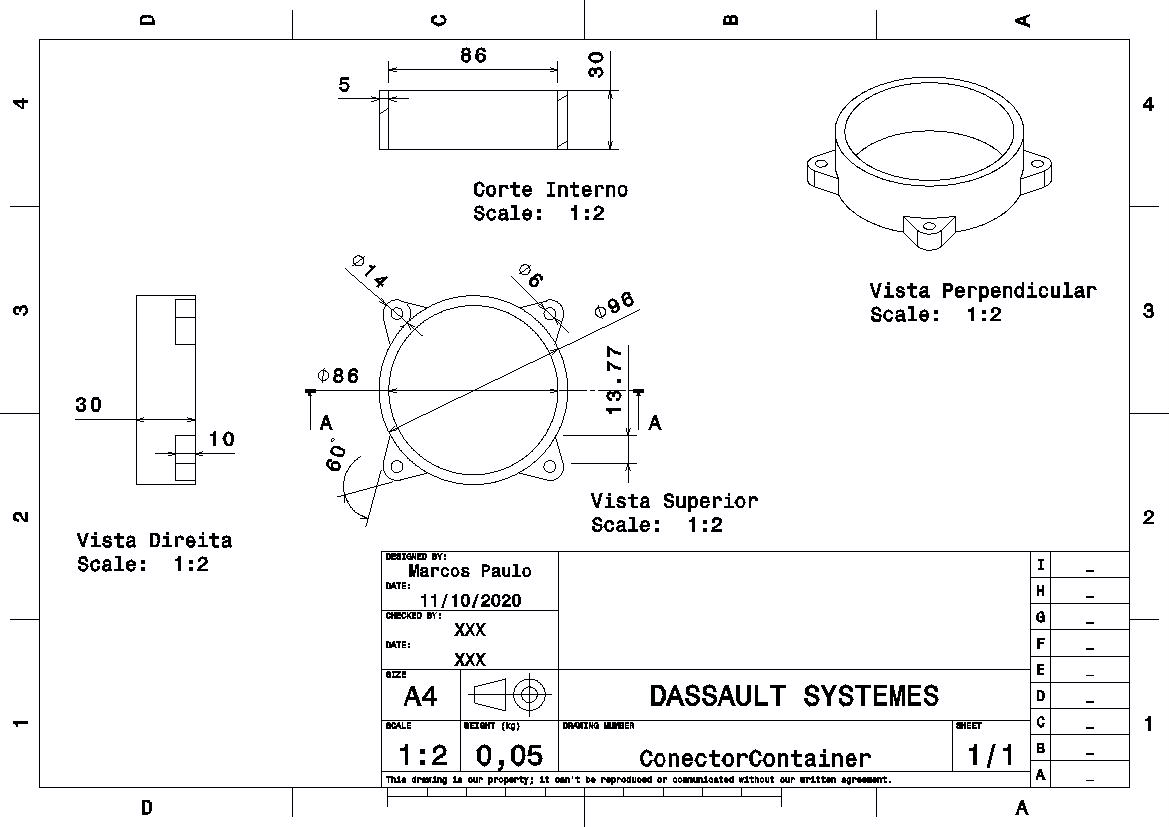
\includegraphics[width=0.9\textwidth]{figuras/estrutura/Desenhos/ConectorContainer.jpg}
    \caption{Desenho técnico do conector do contêiner à base (\ref{retorno_conector})}
    \label{fig:conector}
\end{figure}

\begin{figure}[H]
    \centering
    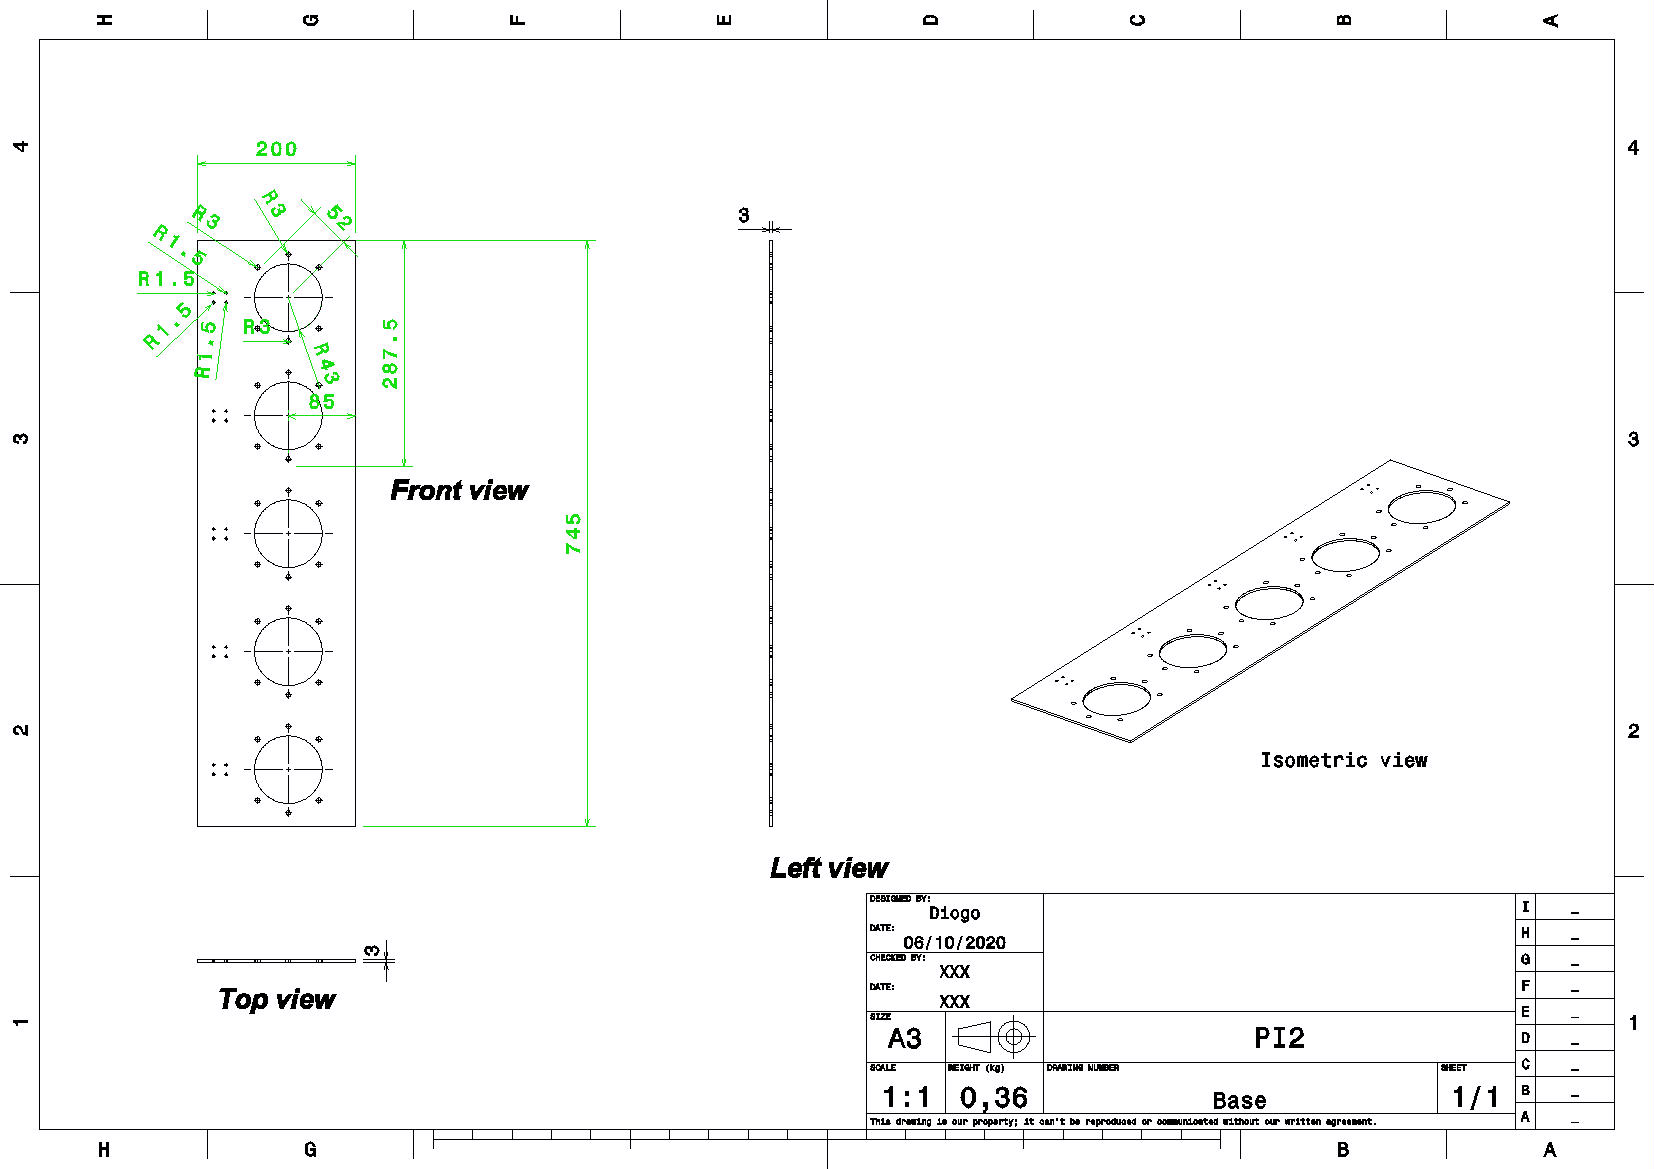
\includegraphics[width=0.9\textwidth]{figuras/estrutura/Desenhos/Drawing1_Base.jpg}
    \caption{Desenho técnico da base dos contêineres (\ref{retorno_base_subgrupo})}
    \label{fig:base_subgrupo}
\end{figure}

\begin{figure}[H]
    \centering
    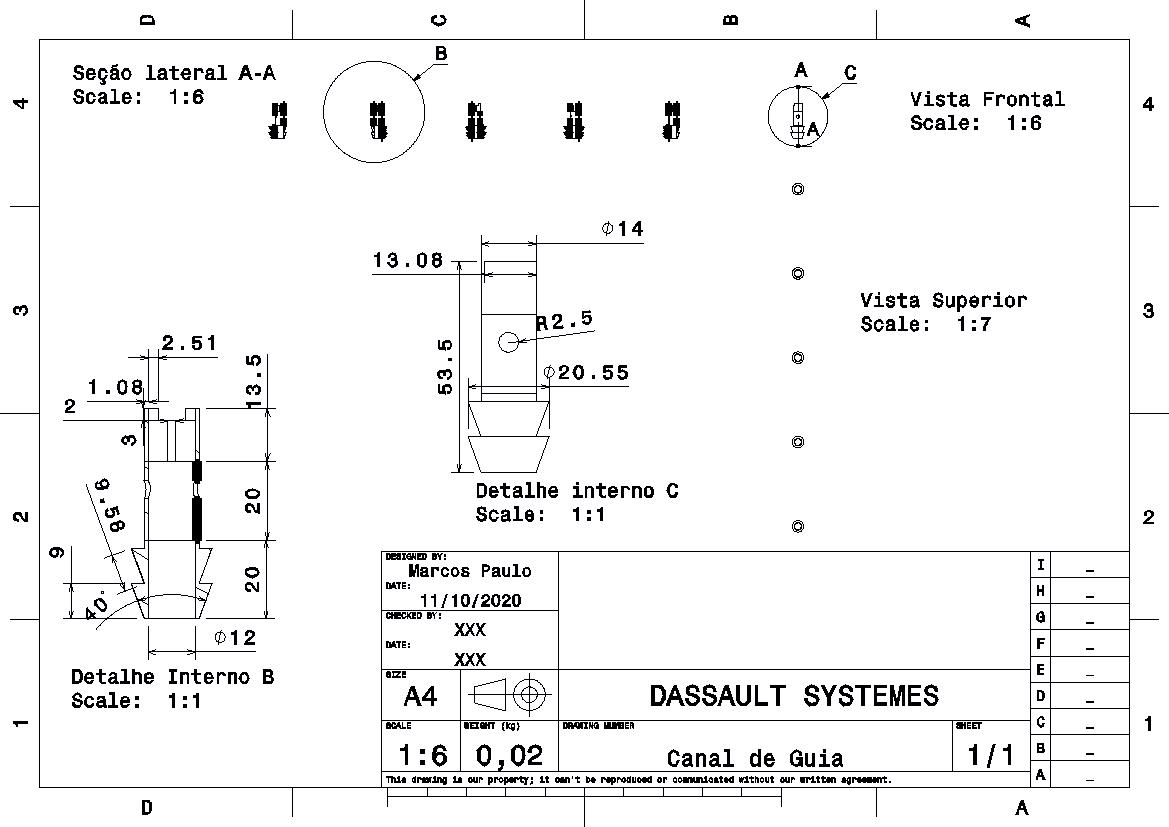
\includegraphics[width=0.9\textwidth]{figuras/estrutura/Desenhos/Canal de Guia.jpg}
    \caption{Desenho técnico do Canal de Guia (\ref{retorno_zonadetransição})}
    \label{fig:canalguia}
\end{figure}

\begin{figure}[H]
    \centering
    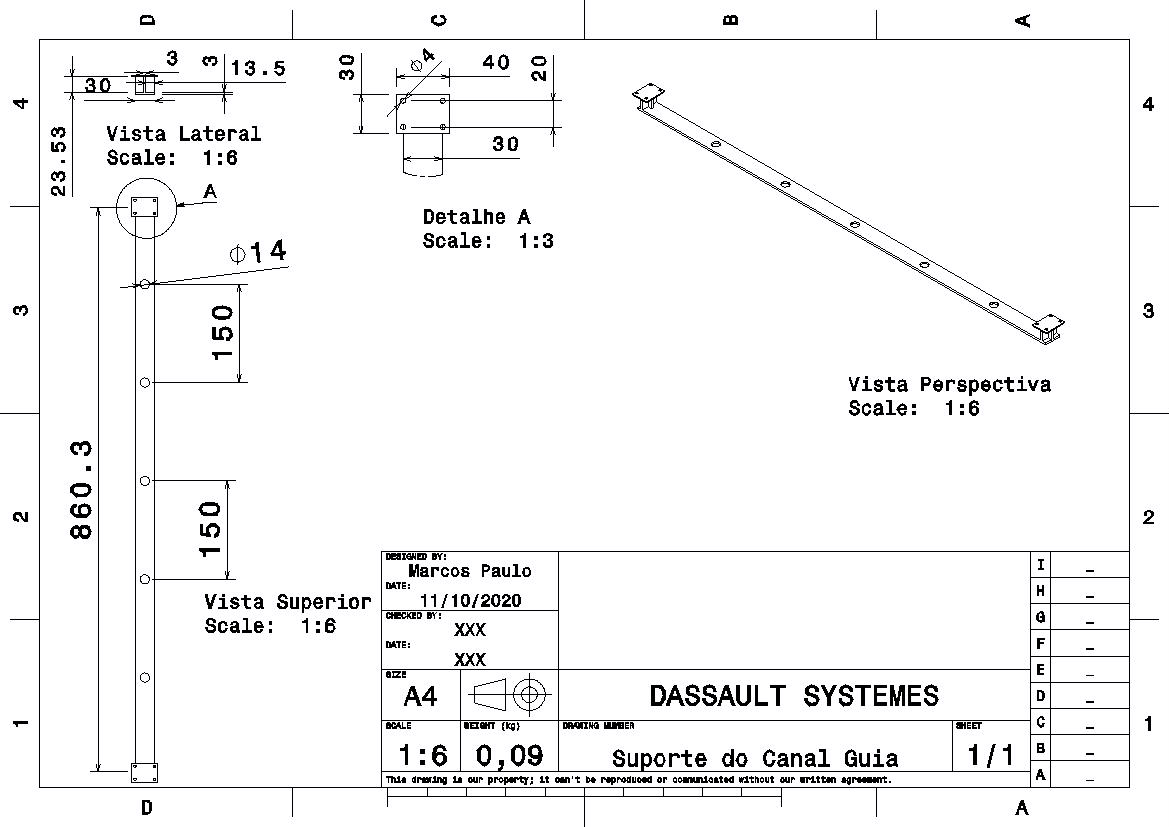
\includegraphics[width=0.9\textwidth]{figuras/estrutura/Desenhos/Suporte_CanaldeGuia.jpg}
    \caption{Desenho técnico do suporte dos canais de guia (\ref{retorno_zonadetransição})}
    \label{fig:supp_canal}
\end{figure}

\begin{figure}[H]
    \centering
    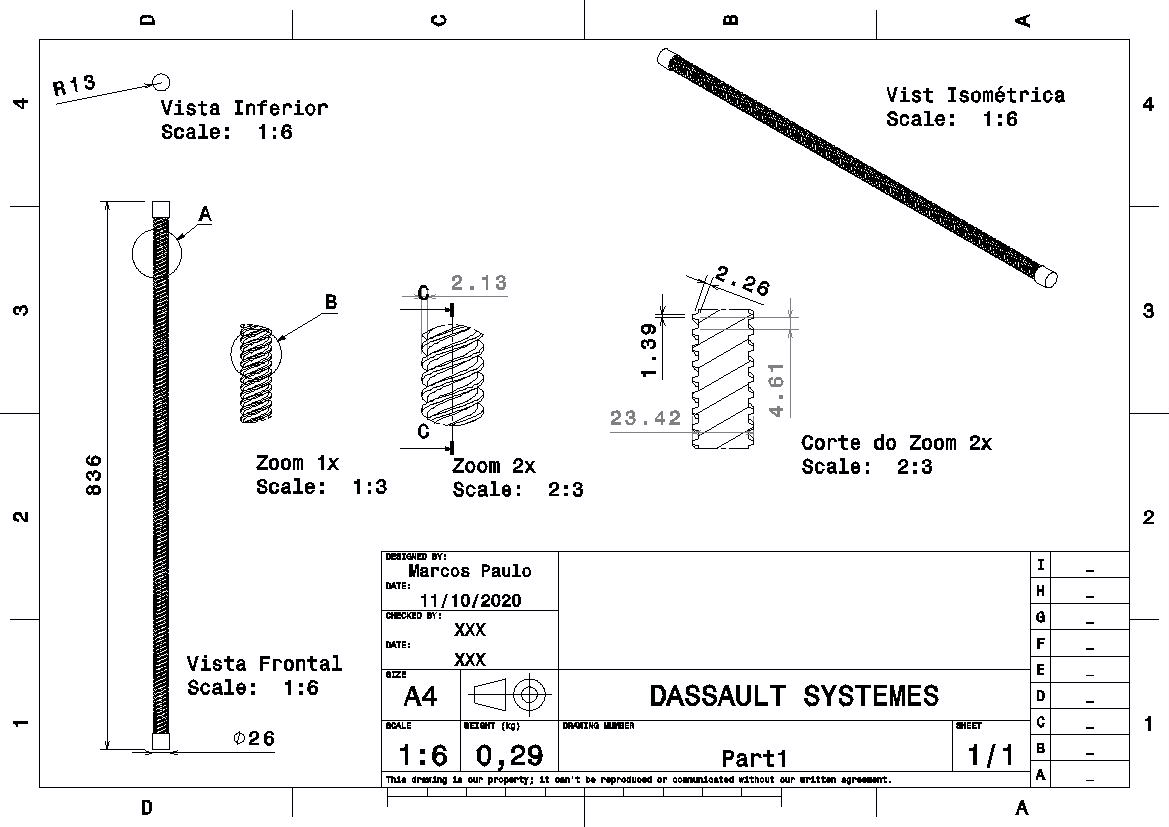
\includegraphics[width=0.9\textwidth]{figuras/estrutura/Desenhos/Fuso_Engrenagens.jpg}
    \caption{Desenho técnico do fuso de atuação nas engrenagens (\ref{retorno_fuso})}
    \label{fig:fuso}
\end{figure}

\begin{figure}[H]
    \centering
    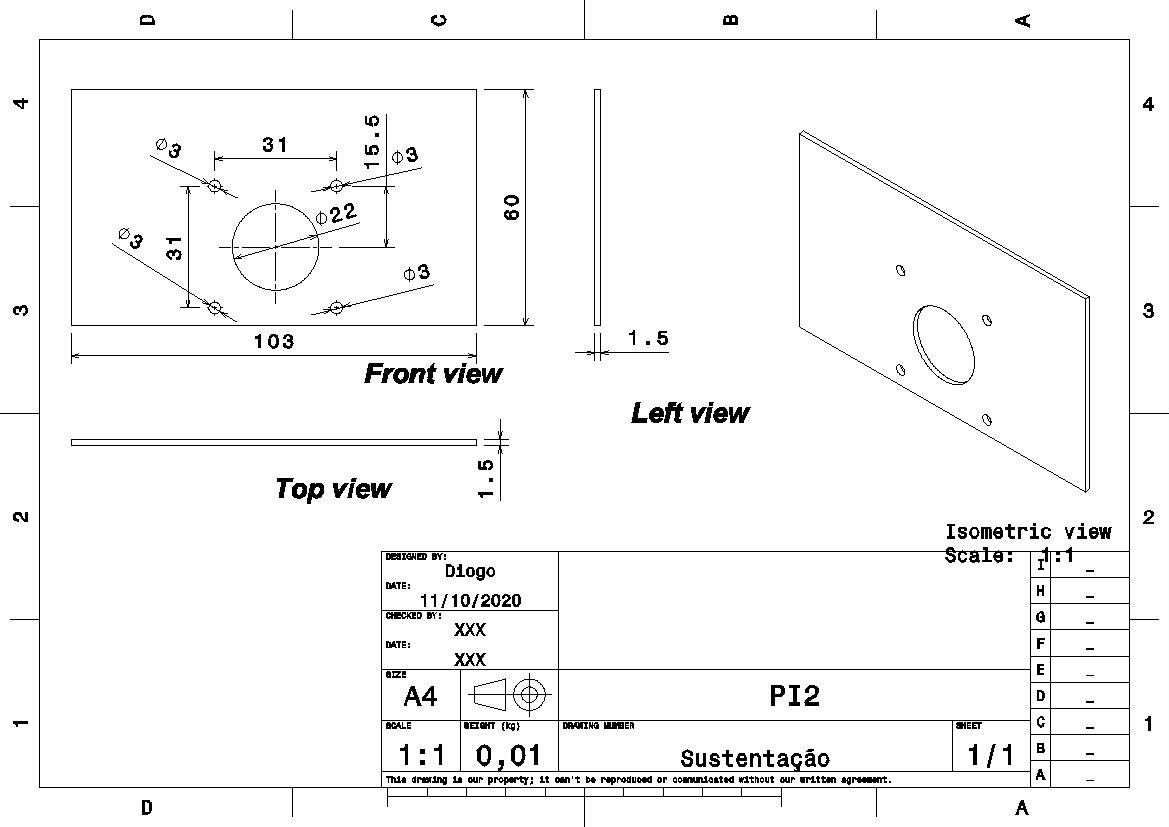
\includegraphics[width=0.9\textwidth]{figuras/estrutura/Desenhos/Sustentação_MotordePasso.jpg}
    \caption{Desenho técnico do suporte dos motores de passo (\ref{retorno_suporte_motordepasso})}
    \label{fig:supp_motordepasso}
\end{figure}

\begin{figure}[H]
    \centering
    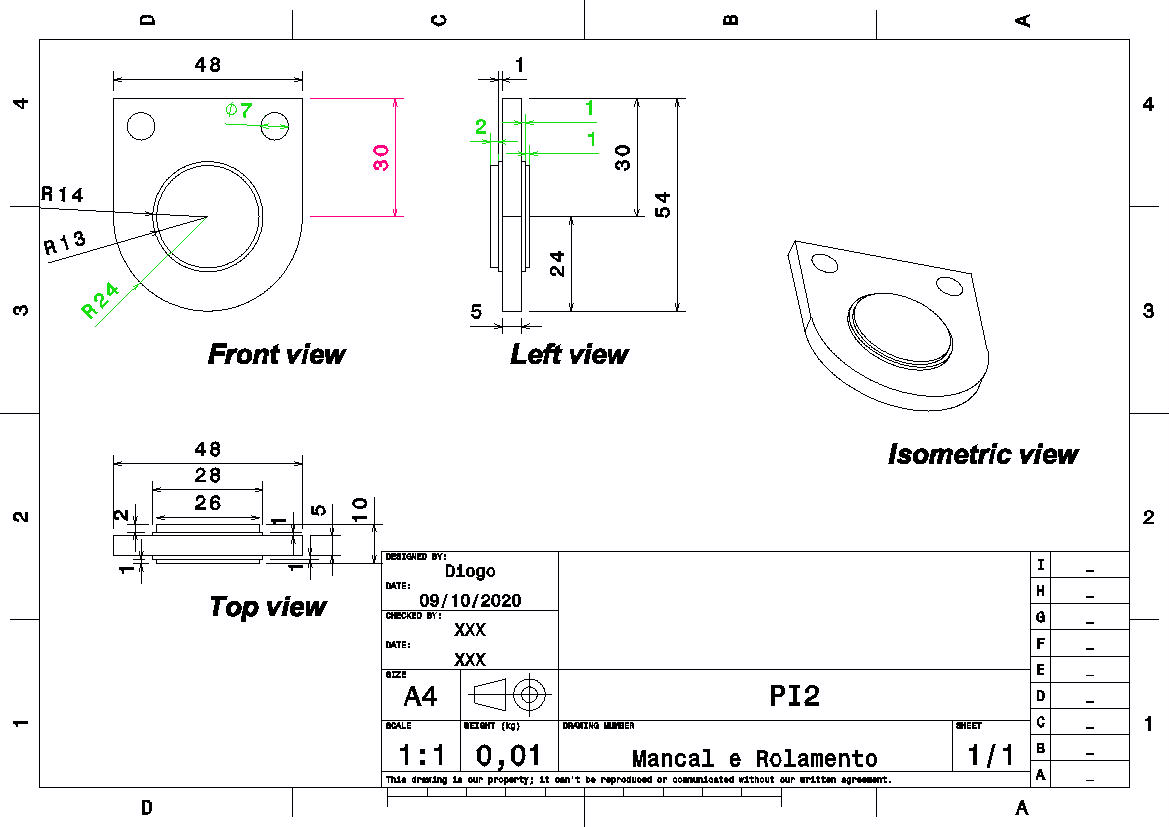
\includegraphics[width=0.9\textwidth]{figuras/estrutura/Desenhos/Drawing1_MacaleRolamento.jpg}
    \caption{Desenho técnico do mancal e rolamento do fuso (\ref{Retorno_Mancal_de_suporte})}
    \label{fig:Mancal_Fuso}
\end{figure}

\begin{figure}[H]
    \centering
    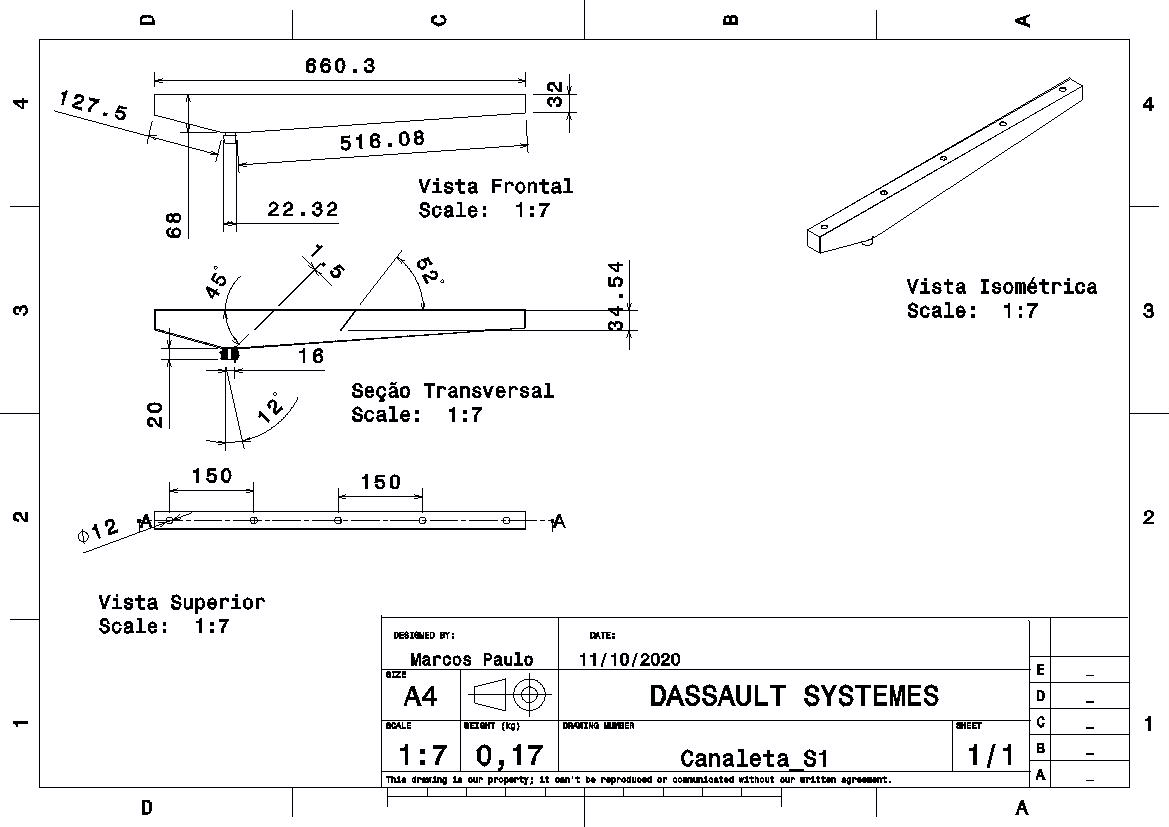
\includegraphics[width=0.9\textwidth]{figuras/estrutura/Desenhos/Canaleta_Subgrupo1.jpg}
    \caption{Desenho técnico da Canaleta do Subgrupo 1 (\ref{retorno_zonadetransição})}
    \label{fig:canaletaS1}
\end{figure}

\begin{figure}[H]
    \centering
    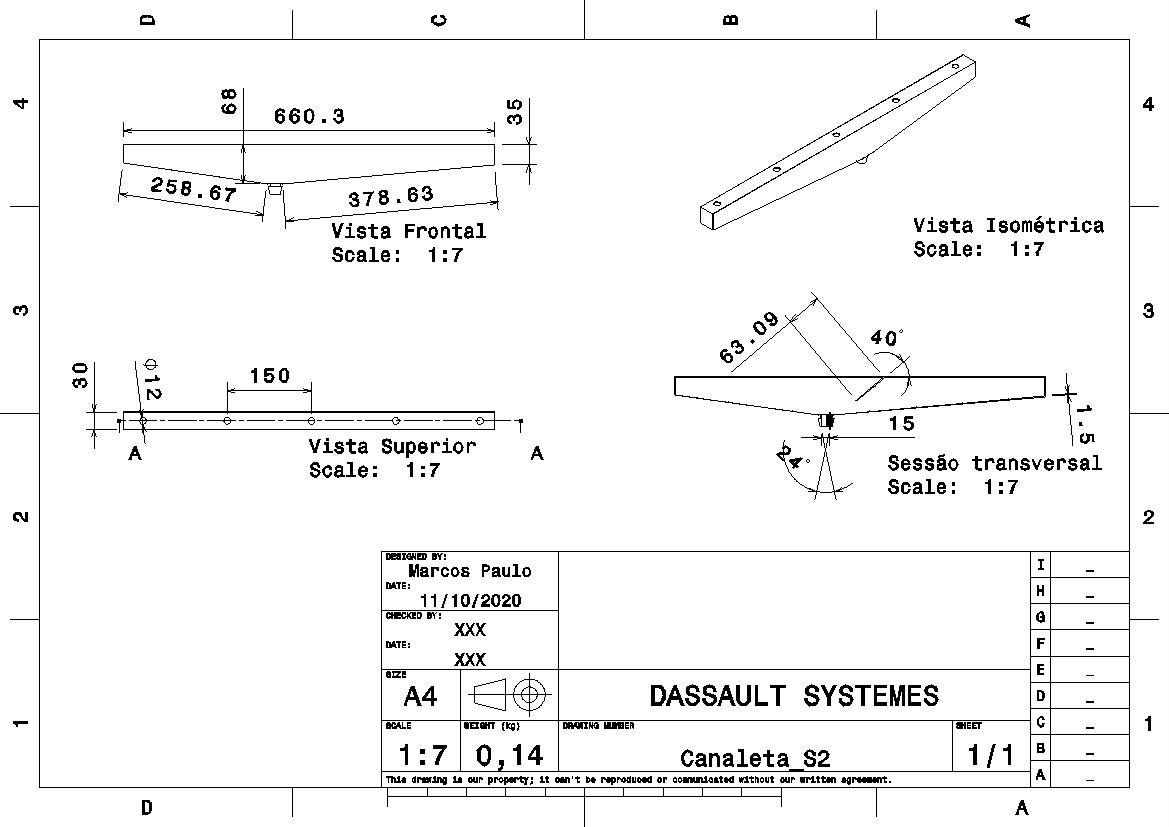
\includegraphics[width=0.9\textwidth]{figuras/estrutura/Desenhos/Canaleta_S2.jpg}
    \caption{Desenho técnico da Canaleta do Subgrupo 2 (\ref{retorno_zonadetransição})}
    \label{fig:canaletaS2}
\end{figure}

\begin{figure}[H]
    \centering
    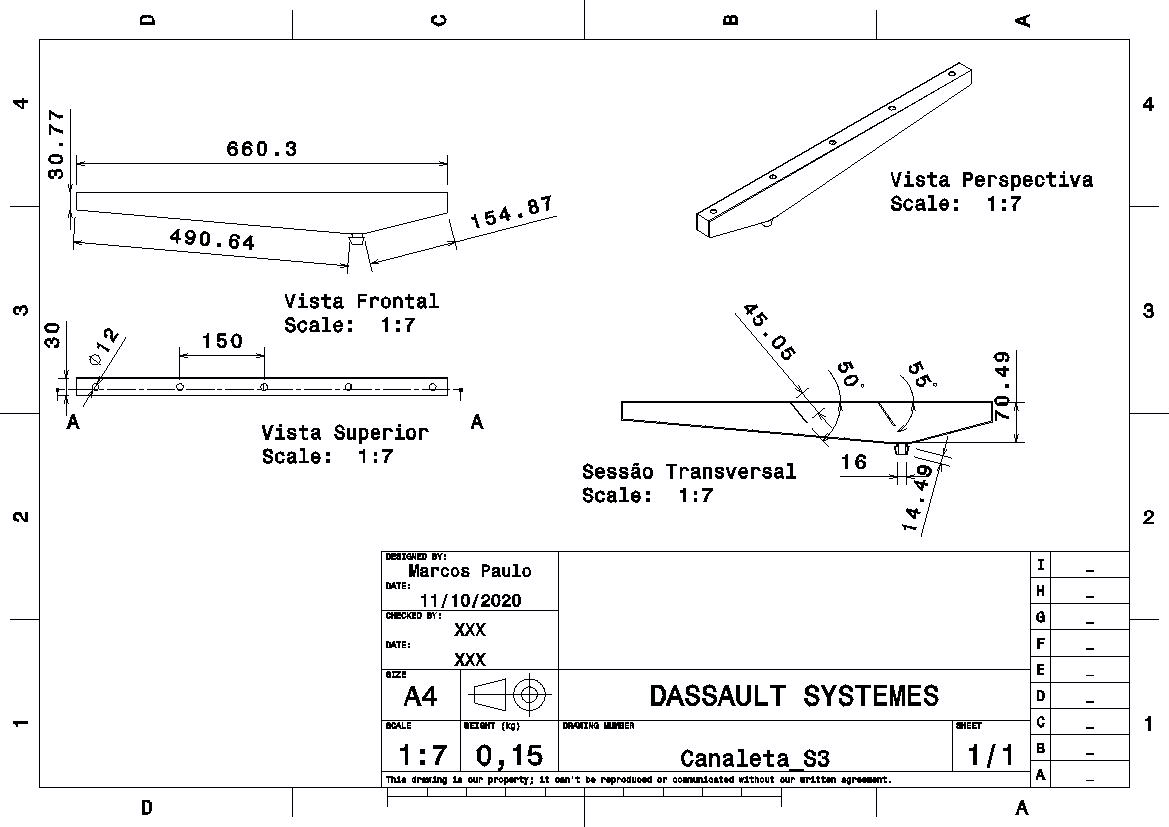
\includegraphics[width=0.9\textwidth]{figuras/estrutura/Desenhos/Canaleta_S3.jpg}
    \caption{Desenho técnico da Canaleta do Subgrupo 3 (\ref{retorno_zonadetransição})}
    \label{fig:canaletaS3}
\end{figure}

\begin{figure}[H]
    \centering
    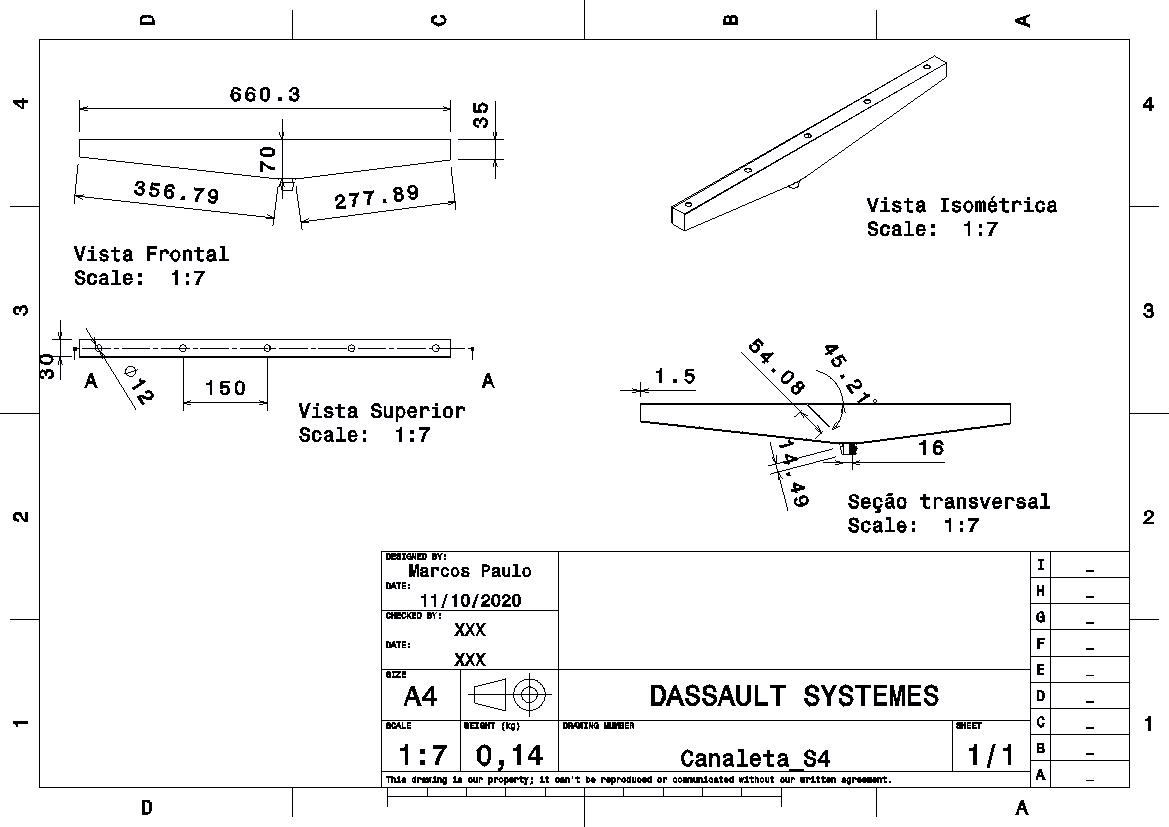
\includegraphics[width=0.9\textwidth]{figuras/estrutura/Desenhos/Canaleta_S4.jpg}
    \caption{Desenho técnico da Canaleta do Subgrupo 4 (\ref{retorno_zonadetransição})}
    \label{fig:canaletaS4}
\end{figure}

\begin{figure}[H]
    \centering
    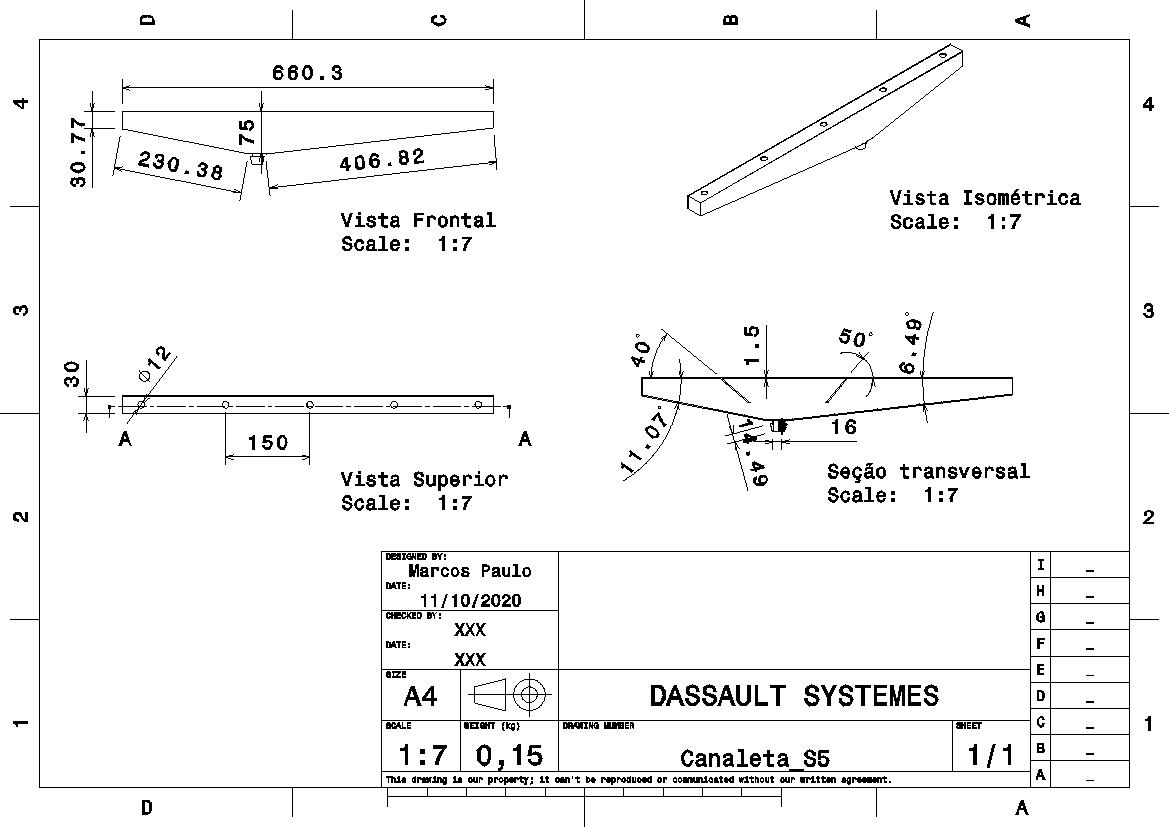
\includegraphics[width=0.9\textwidth]{figuras/estrutura/Desenhos/Canaleta_S5.jpg}
    \caption{Desenho técnico da Canaleta do Subgrupo 5 (\ref{retorno_zonadetransição})}
    \label{fig:canaletaS5}
\end{figure}

\begin{figure}[H]
    \centering
    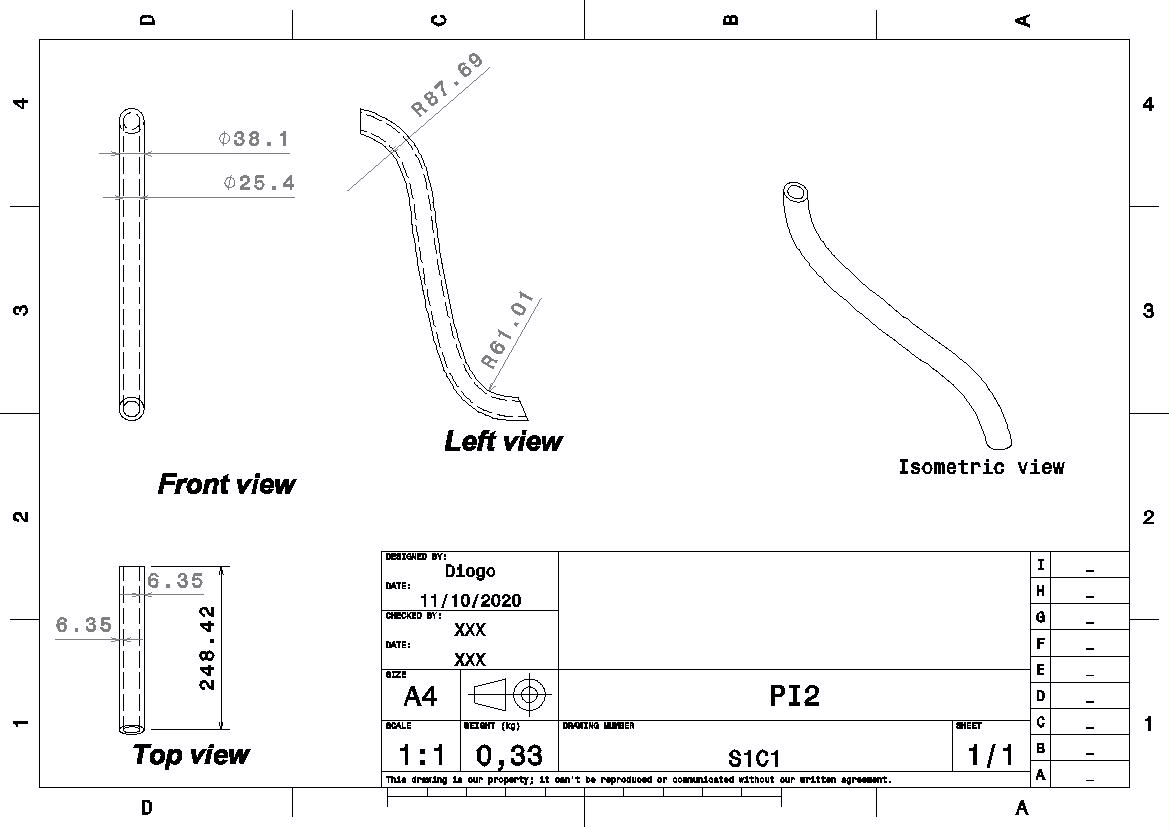
\includegraphics[width=0.9\textwidth]{figuras/estrutura/Desenhos/Drawing1_S1C1.jpg}
    \caption{Desenho técnico da mangueira do subgrupo 1 (\ref{retorno_mangueira})}
    \label{fig:M_S1}
\end{figure}

\begin{figure}[H]
    \centering
    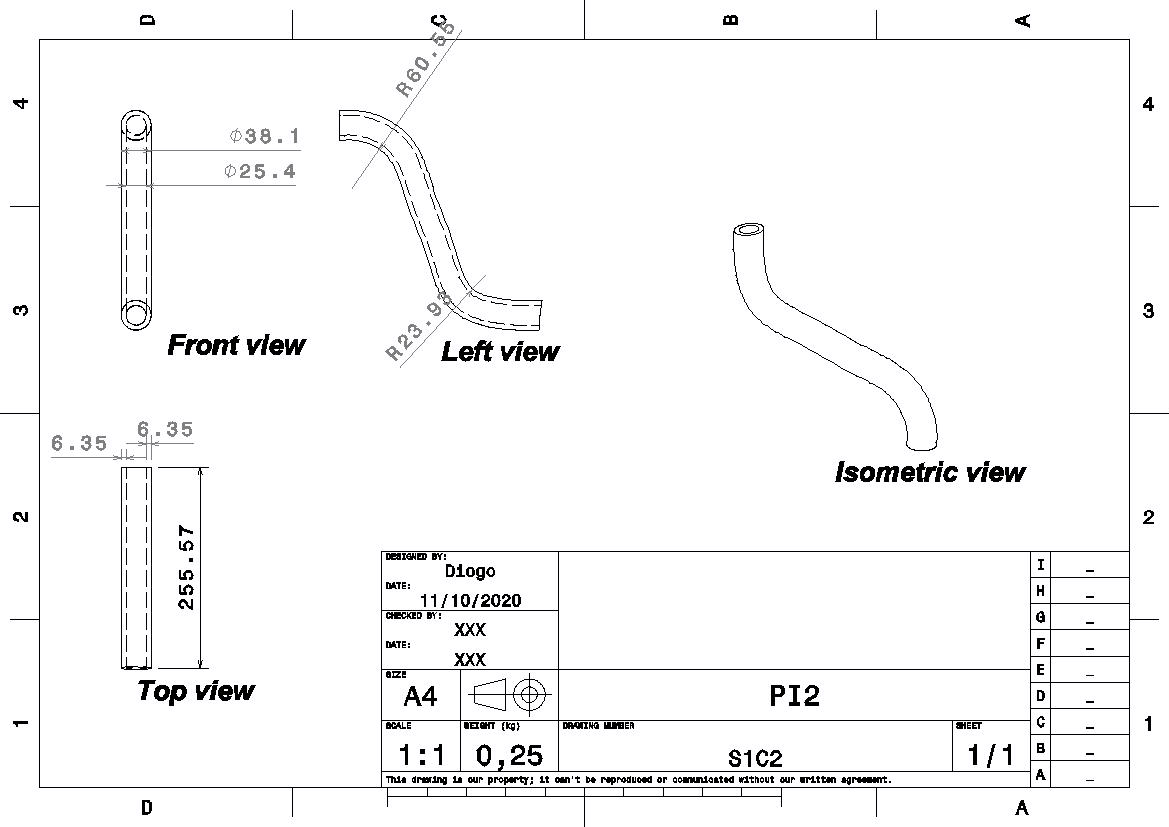
\includegraphics[width=0.9\textwidth]{figuras/estrutura/Desenhos/Drawing1_S1C2.jpg}
    \caption{Desenho técnico da mangueira do subgrupo 2 (\ref{retorno_mangueira})}
    \label{fig:M_S2}
\end{figure}

\begin{figure}[H]
    \centering
    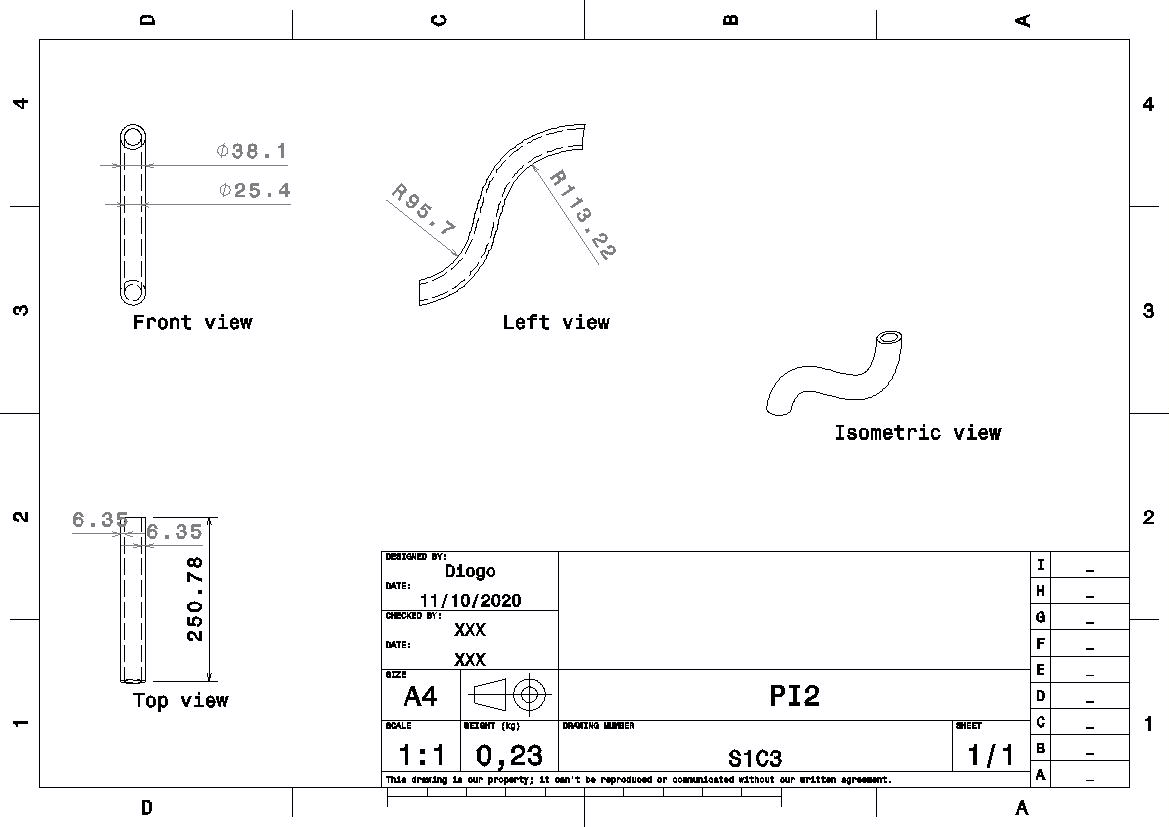
\includegraphics[width=0.9\textwidth]{figuras/estrutura/Desenhos/Drawing1_S1C3.jpg}
    \caption{Desenho técnico da mangueira do subgrupo 3 (\ref{retorno_mangueira})}
    \label{fig:M_S3}
\end{figure}

\begin{figure}[H]
    \centering
    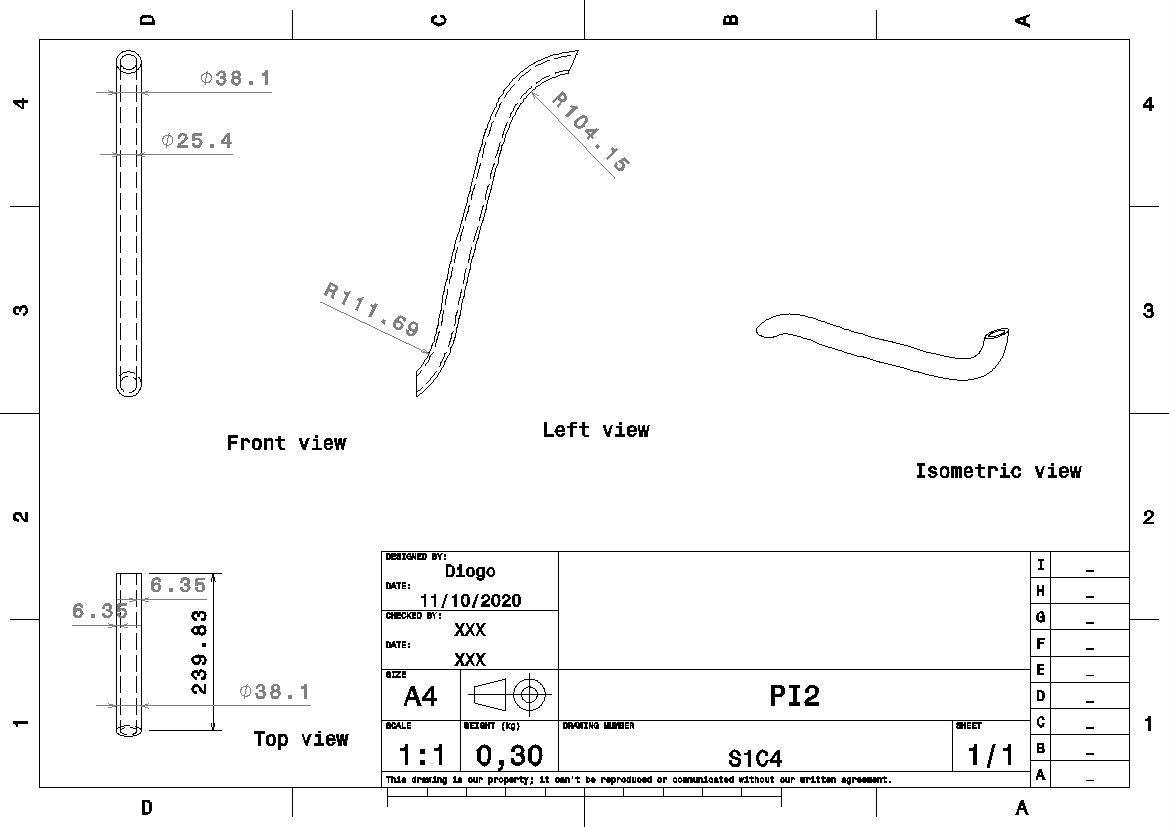
\includegraphics[width=0.9\textwidth]{figuras/estrutura/Desenhos/Drawing1_S1C4.jpg}
    \caption{Desenho técnico da mangueira do subgrupo 4 (\ref{retorno_mangueira})}
    \label{fig:M_S4}
\end{figure}

\begin{figure}[H]
    \centering
    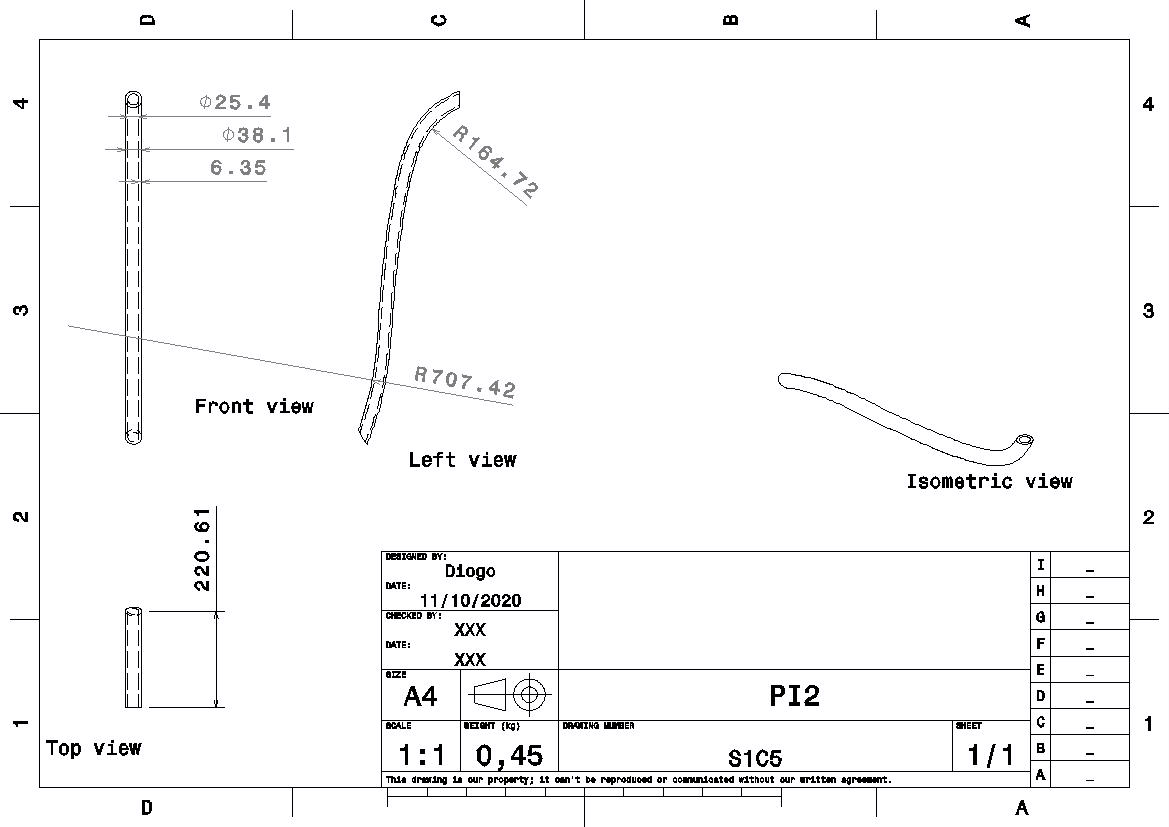
\includegraphics[width=0.9\textwidth]{figuras/estrutura/Desenhos/Drawing1_S1C5.jpg}
    \caption{Desenho técnico da mangueira do subgrupo 5 (\ref{retorno_mangueira})}
    \label{fig:M_S5}
\end{figure}

\begin{figure}[H]
    \centering
    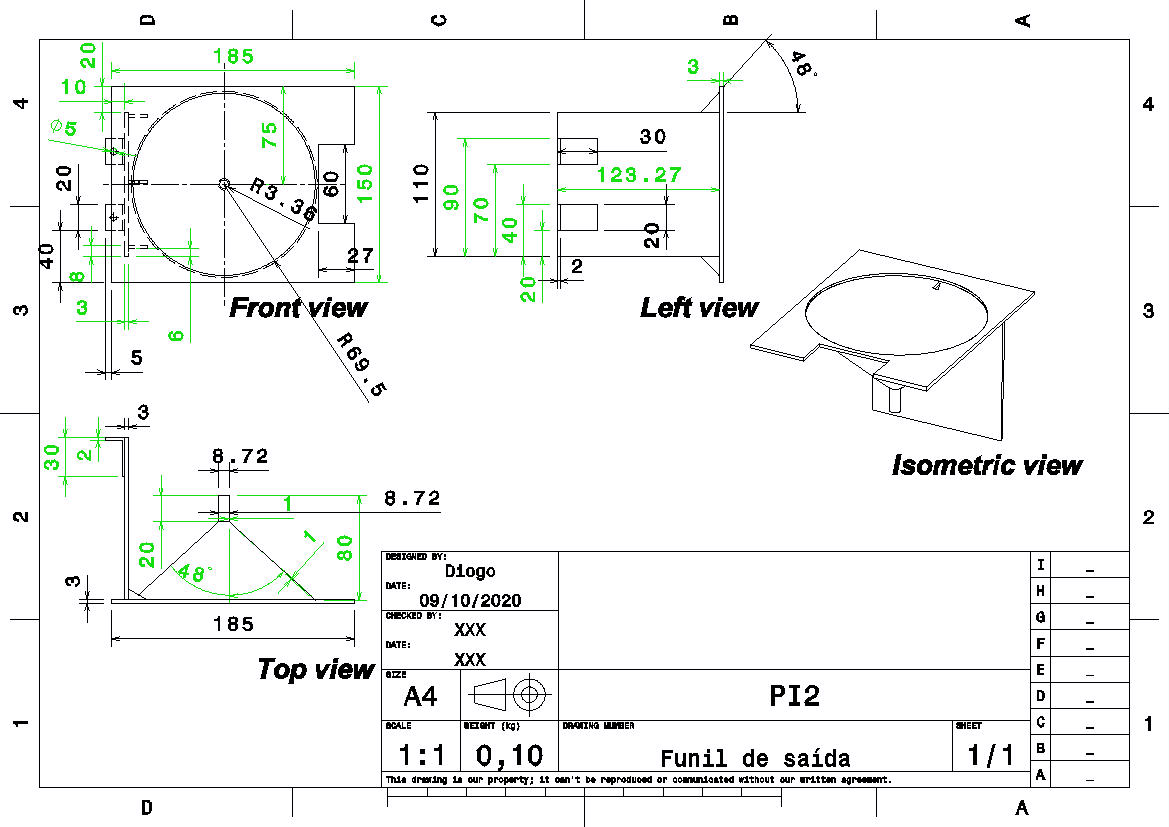
\includegraphics[width=0.9\textwidth]{figuras/estrutura/Desenhos/Drawing1_FunildeSaida.jpg}
    \caption{Desenho técnico do funil de saída das mangueiras (\ref{retorno_funil})}
    \label{fig:funil}
\end{figure}

\begin{figure}[H]
    \centering
    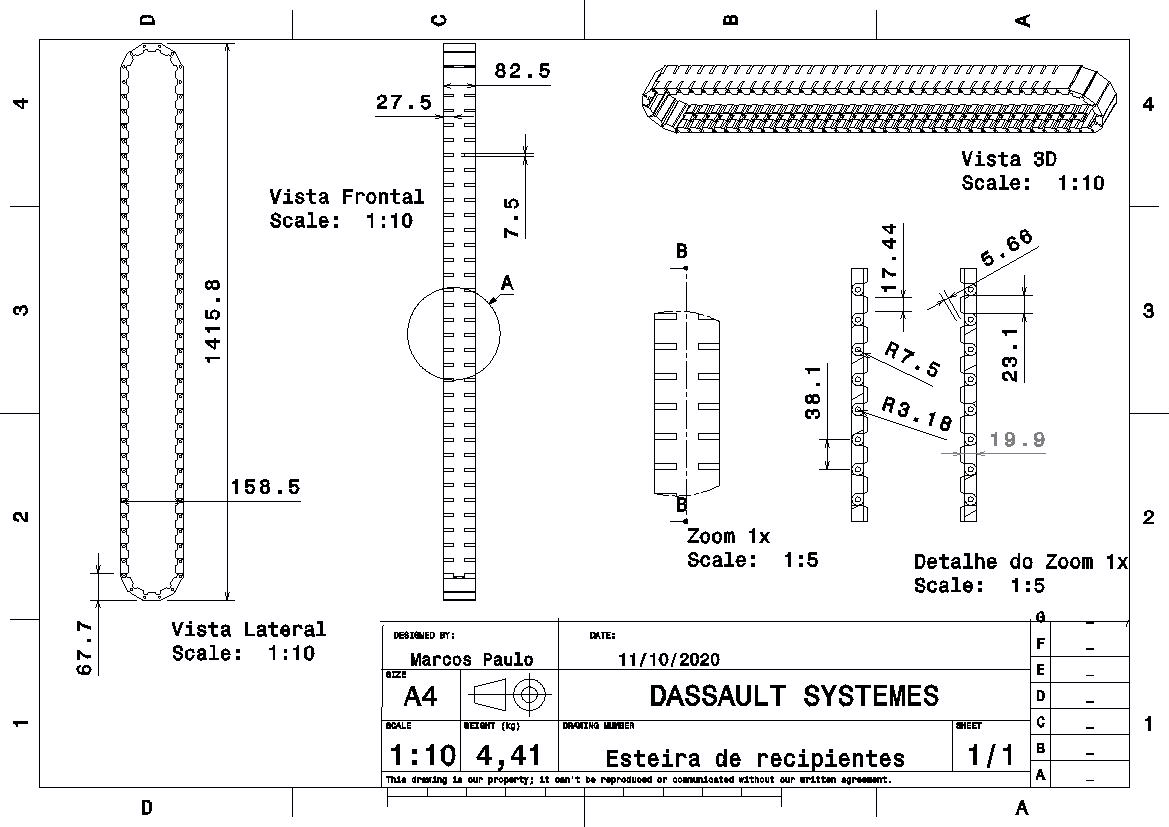
\includegraphics[width=0.9\textwidth]{figuras/estrutura/Desenhos/Esteira.jpg}
    \caption{Desenho técnico da esteira dos copos (\ref{retorno_esteira})}
    \label{fig:esteira}
\end{figure}

\begin{figure}[H]
    \centering
    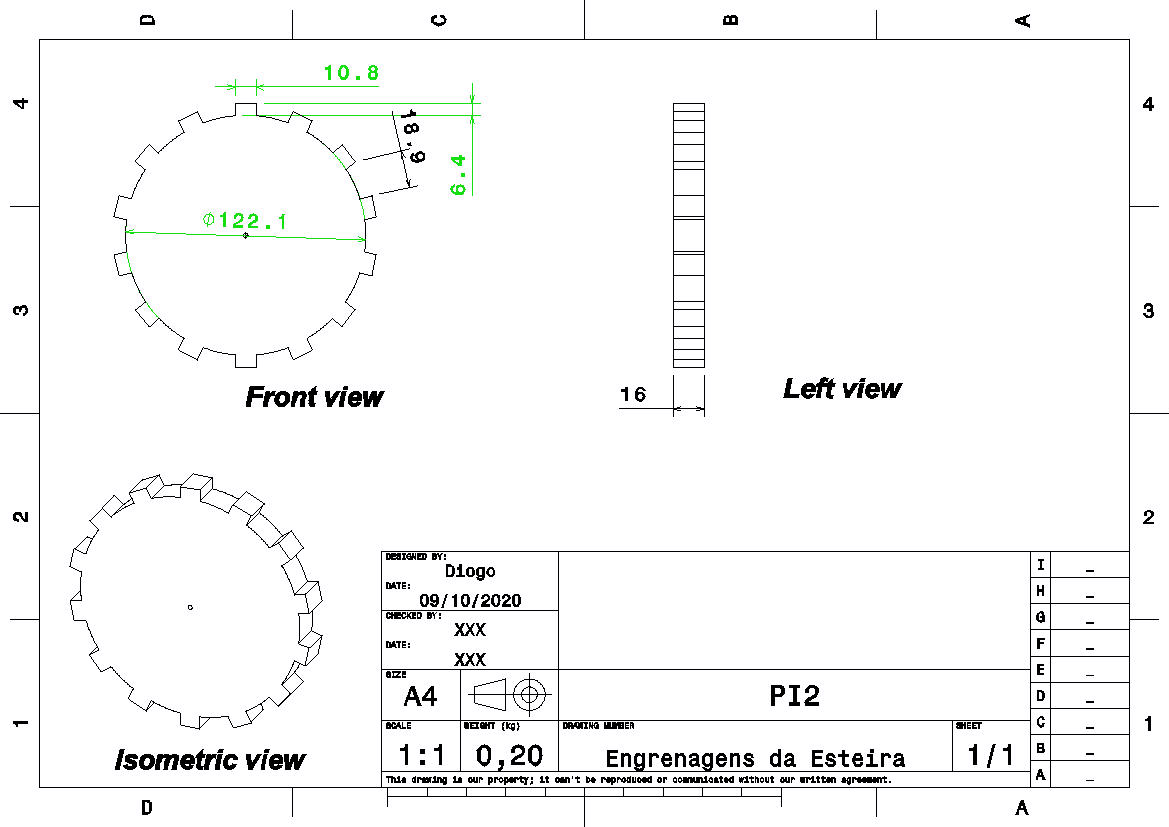
\includegraphics[width=0.9\textwidth]{figuras/estrutura/Desenhos/Drawing1_EngrenagemdaEsteira2.jpg}
    \caption{Desenho técnico da engrenagem da esteira (\ref{retorno_esteira})}
    \label{fig:engrenagem_esteira}
\end{figure}

\begin{figure}[H]
    \centering
    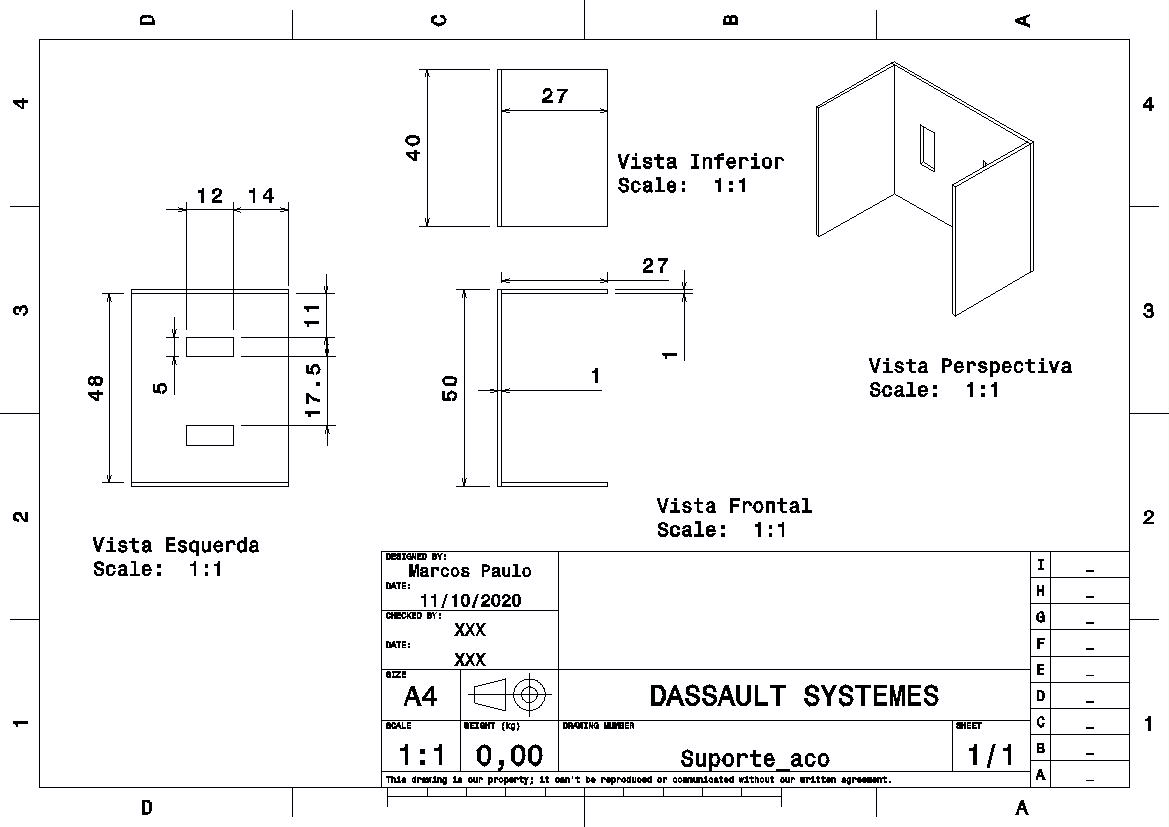
\includegraphics[width=0.9\textwidth]{figuras/estrutura/Desenhos/Suporte_MotorDC.jpg}
    \caption{Desenho técnico do suporte do motor DC da esteira (\ref{Retorno_suporte_motorDC})}
    \label{fig:supp_motordc}
\end{figure}

\begin{figure}[H]
    \centering
    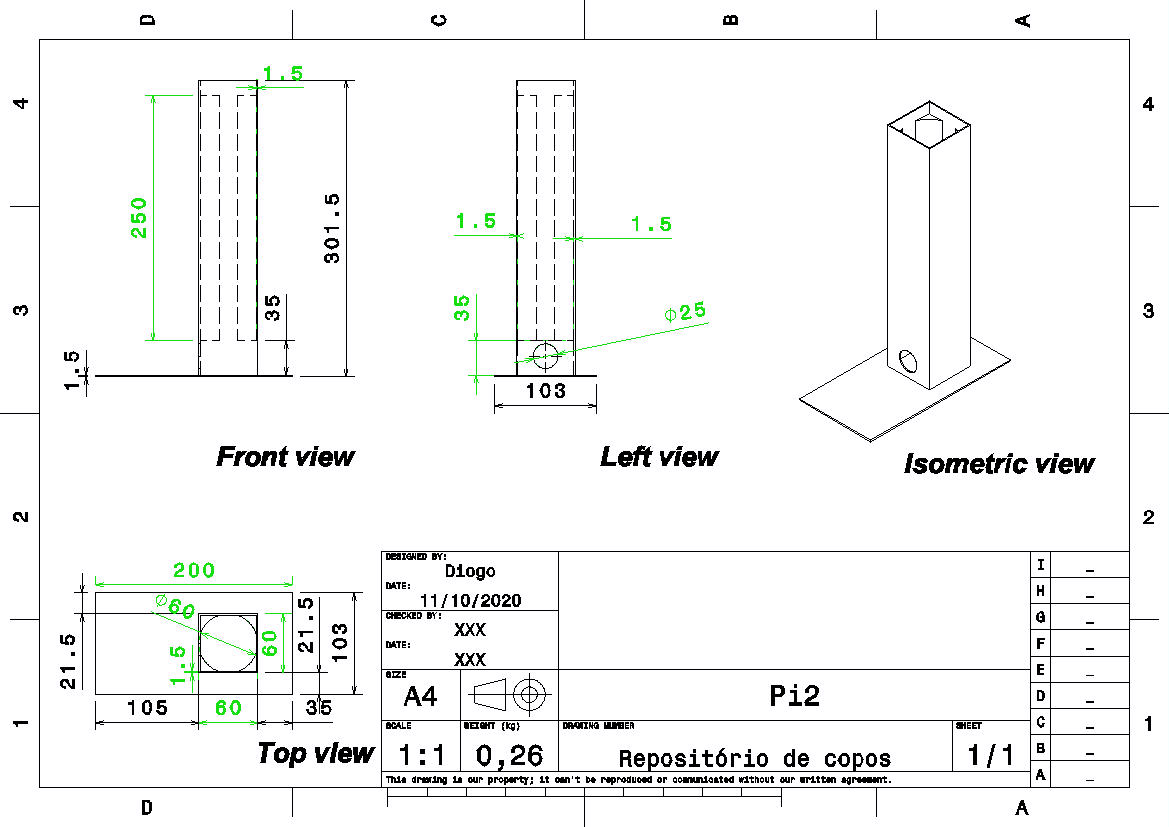
\includegraphics[width=0.9\textwidth]{figuras/estrutura/Desenhos/Drawing1_RepositoriodeCopos.jpg}
    \caption{Desenho técnico do repositório de copos (\ref{retorno_reservatorio})}
    \label{fig:repositorio}
\end{figure}

\begin{figure}[H]
    \centering
    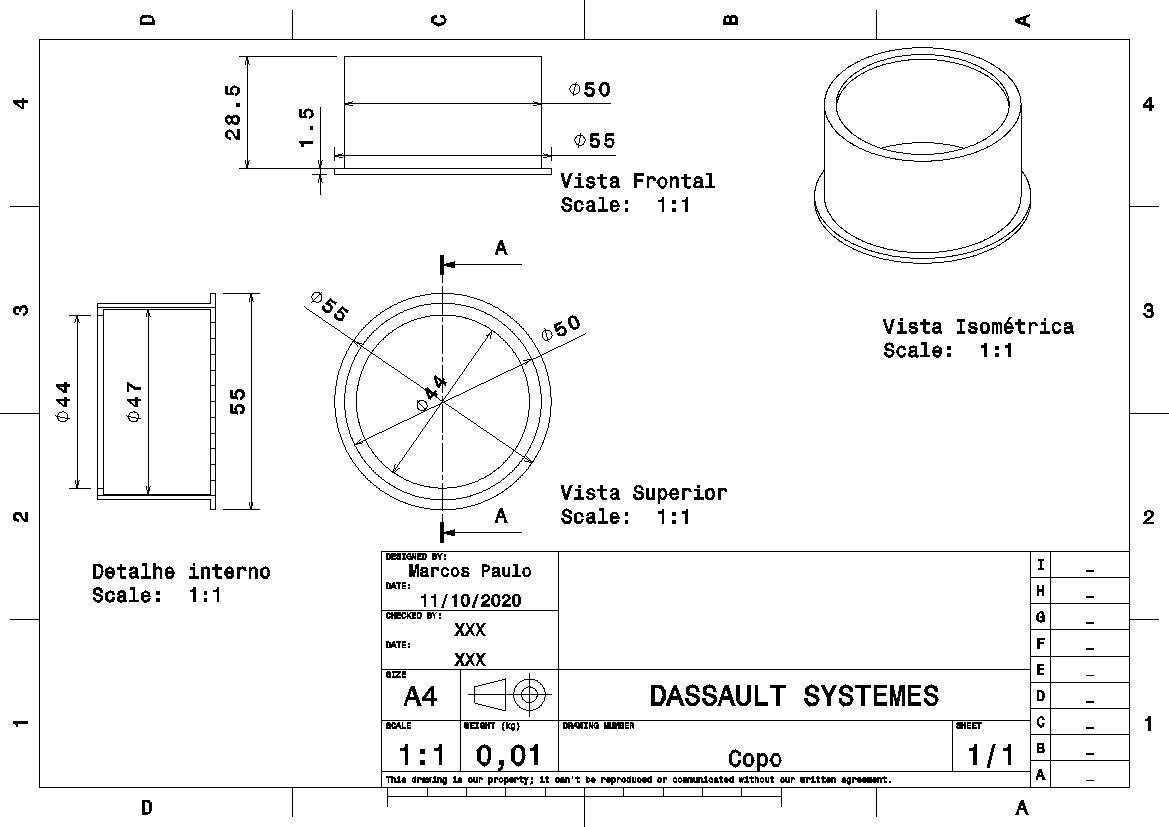
\includegraphics[width=0.9\textwidth]{figuras/estrutura/Desenhos/Copo.jpg}
    \caption{Desenho técnico do copo de medicamentos (\ref{retorno_copo})}
    \label{fig:copo}
\end{figure}

\begin{figure}[H]
    \centering
    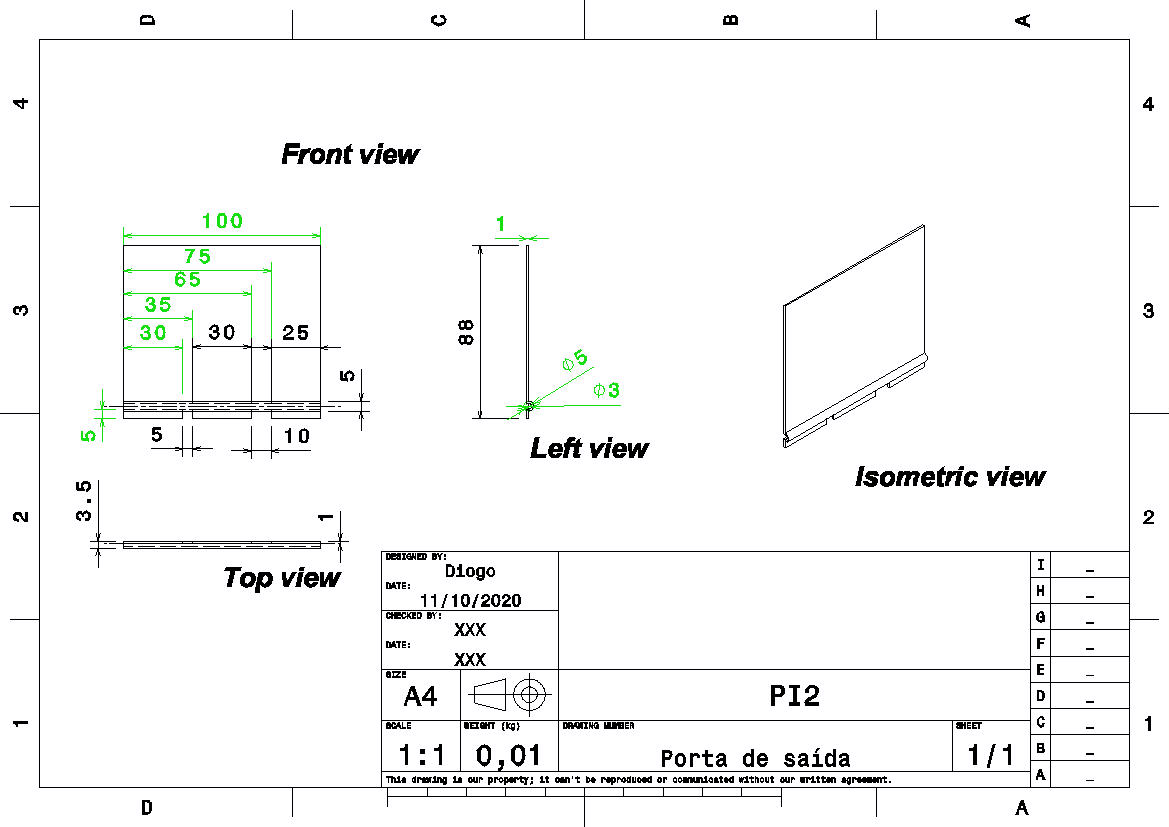
\includegraphics[width=0.9\textwidth]{figuras/estrutura/Desenhos/Drawing1_PortadeSaida.jpg}
    \caption{Desenho técnico da porta de saída, que se apresenta tanto na saída verdadeira quanto na sáida de retorno (\ref{retorno_porta})}
    \label{fig:porta_saida}
\end{figure}

\begin{figure}[H]
    \centering
    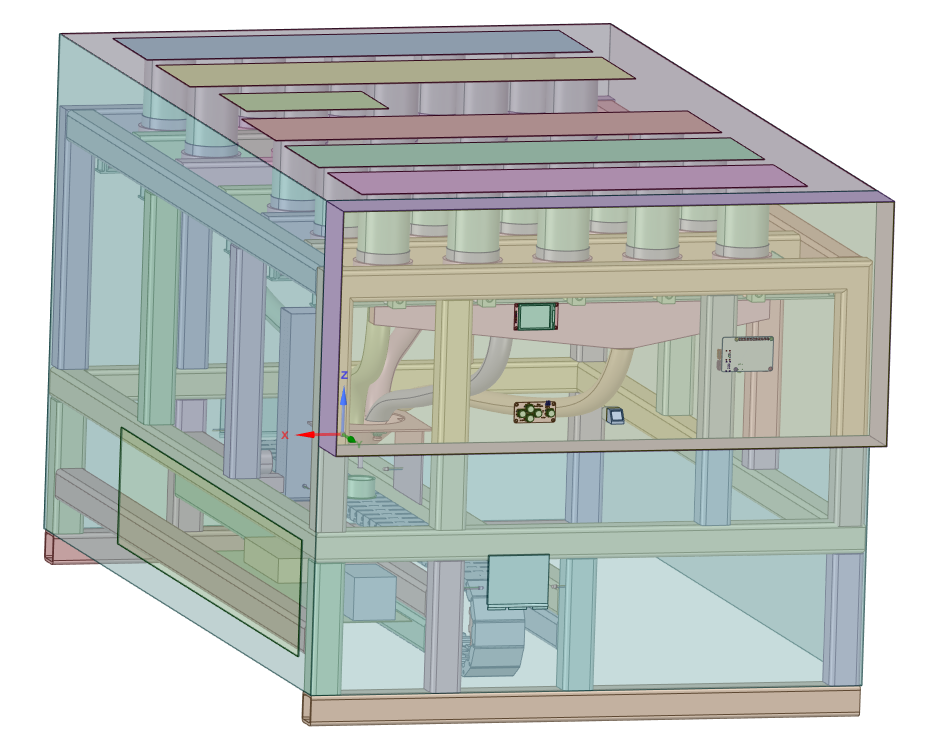
\includegraphics[width=0.9\textwidth]{figuras/estrutura/Design/Vista completa com circuitaria.png}
    \caption{Estrutural Global em formato CAD}
    \label{fig:global}
\end{figure}

\begin{figure}[H]
    \centering
    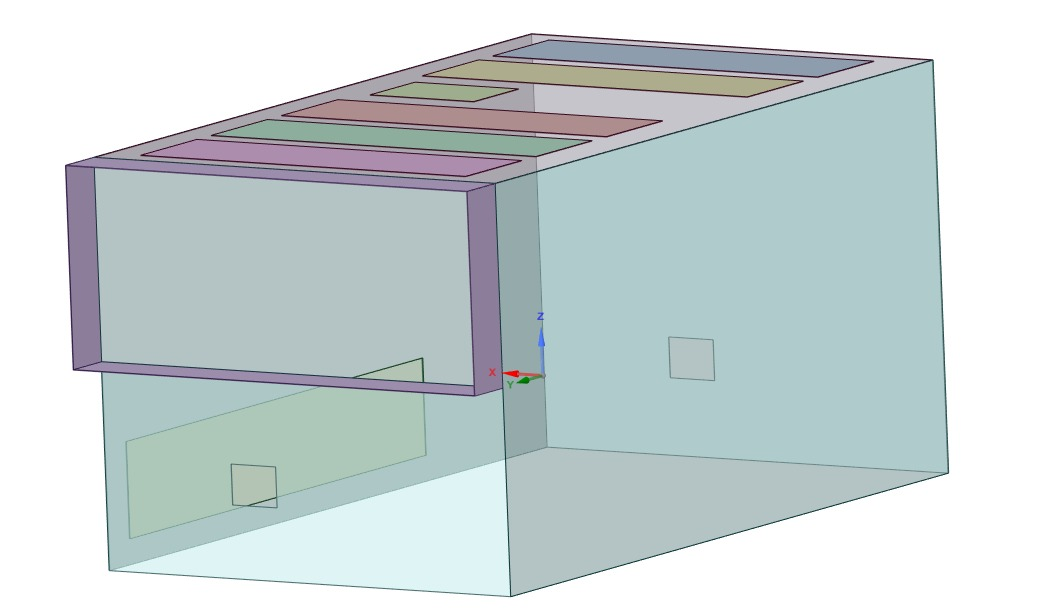
\includegraphics[width=0.7\textwidth]{figuras/estrutura/Design/ChapasExterior.jpeg}
    \caption{Carcaça da estrutura formato CAD}
    \label{fig:Carcaca}
\end{figure}

\begin{figure}[H]
    \centering
    \includegraphics[width=0.7\textwidth]{figuras/estrutura/Porta de saída.png}
    \caption{Porta de saída}
    \label{fig:portas}
\end{figure}

\begin{figure}[H]
    \centering
    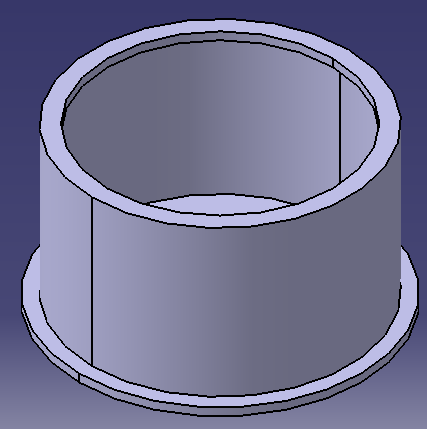
\includegraphics[width=0.7\textwidth]{figuras/estrutura/Copo.png}
    \caption{Ilustração do Copo}
    \label{fig:copos}
\end{figure}

\begin{figure}[H]
    \centering
    \includegraphics[width=0.9\textwidth]{figuras/estrutura/Motor DC na Esteira.png}
    \caption{Motor DC na esteira}
    \label{fig:DCnaesteira}
\end{figure}

\begin{figure}[H]
    \centering
    \includegraphics[width=1\textwidth]{figuras/estrutura/Motor de Passo no Fuso.png}
    \caption{Motor de passo com fuso}
    \label{fig:motordepassonofuso}
\end{figure}

\begin{figure}[H]
    \centering
    \includegraphics[width=0.9\textwidth]{figuras/estrutura/Recipiente dos Copos + Esteira.png}
    \caption{Reservatório de copos com esteira}
    \label{fig:reservatorioCopos}
\end{figure}

\begin{figure}[H]
    \centering
    \includegraphics[width=0.9\textwidth]{figuras/estrutura/Detalhe Fuso com Engrenagem.png}
    \caption{Detalhes do fuso com engrenagens}
    \label{fig:fusoEngrenagens}
\end{figure}   

\begin{figure}[H]
    \centering
    \includegraphics[width=0.7\textwidth]{figuras/estrutura/Conteiner.png}
    \caption{Contêiner dos medicamentos}
    \label{fig:conteiner}
\end{figure}

\begin{figure}[H]
    \centering
    \includegraphics[width=0.6\textwidth]{figuras/estrutura/Descrição Contêiner.png}
    \caption{Descrição detalhada do contêiner}
    \label{fig:DescricaoConteiner}
\end{figure}

%\begin{figure}[H]
%    \centering
%    \includegraphics[width=0.8\textwidth]{figuras/estrutura/Perfil Quadrado.png}
%    \caption{Cotagem do Tubo}
%    \label{fig:Cotastubo}
%\end{figure}    

\chapter{\textit{Mockup} das Telas do \textit{Display}}\label{app_telas_display}

A Central de Controle exibirá no \textit{display} para usuário os avisos e status dos sistemas que compõem o projeto. Assim, para a inicialização do dispositivo deve-se realizar o cadastro no aplicativo do número de série disponível no \textit{display}, conforme a figura \ref{fig:app_tela_1}. Em seguida o usuário irá selecionar uma rede de internet para fazer o login, segundo a figura \ref{fig:app_tela_2}. Posteriormente, deve-se digitar a senha por meio da utilização da matriz de botões no teclado virtual disponível no \textit{display}, na figura \ref{fig:app_tela_3}. 

\begin{figure}[H]
    \centering
    \subfloat[][Tela Inicial com Número de série]{
    \includegraphics[width=4.3cm]{figuras/Telas/1.png}
    \label{fig:app_tela_1}}
    \subfloat[][Tela de seleção Inicial de Rede]{
    \includegraphics[width=4.3cm]{figuras/Telas/2.png}
    \label{fig:app_tela_2}}
    \subfloat[][Tela de conexão]{
    \includegraphics[width=4.3cm]{figuras/Telas/3.png}
    \label{fig:app_tela_3}}
    \caption{Telas de Iniciação}\label{fig:telas_1_2_3}
\end{figure}

A figura \ref{fig:app_tela_4} apresenta a tela inicial no modo de espera, com horário, data, item de conexão com a internet, item da conexão do dispositivo com a rede elétrica e quando o dispositivo utiliza a bateria, em casos de falta de energia. Além do mais, a partir da tela inicial, é possível acessar as configurações e a agenda de medicamentos. Assim, conforme a figura \ref{fig:app_tela_24}, existe a representação da agenda na próxima uma hora de medicações dos pacientes por ordem de horário.

\begin{figure}[H]
    \centering
    \subfloat[][Tela Inicial]{
    \includegraphics[width=4.3cm]{figuras/Telas/4.png}
    \label{fig:app_tela_4}}
    \subfloat[][Tela da agenda com medicações]{
    \includegraphics[width=4.3cm]{figuras/Telas/24.png}
    \label{fig:app_tela_24}}
    \caption{Tela Inicial e Tela da Agenda}\label{fig:telas_4_24}
\end{figure}

Ao clicar, utilizando a matriz de botões no ícone das configurações, o usuário é encaminhado para um menu \ref{fig:app_tela_9}. Nele é possível alterar a rede de conexão com a internet \ref{fig:app_tela_10}, alterar data e hora \ref{fig:app_tela_11}, alterar o brilho da tela \ref{fig:app_tela_12} e acessar a tela com informações técnicas do dispositivo \ref{fig:app_tela_13}.

\begin{figure}[H]
    \centering
    \subfloat[][Tela de configurações]{
    \includegraphics[width=4.3cm]{figuras/Telas/9.png}
    \label{fig:app_tela_9}}
    \subfloat[][Tela de alteração de rede]{
    \includegraphics[width=4.3cm]{figuras/Telas/10.png}
    \label{fig:app_tela_10}}
    \subfloat[][Tela de alteração da data e hora]{
    \includegraphics[width=4.3cm]{figuras/Telas/11.png}
    \label{fig:app_tela_11}}
    \caption{Telas de Configuração - Parte 1}\label{fig:telas_9_10_11}
\end{figure}

\begin{figure}[H]
    \centering
    \subfloat[][Tela de alteração do brilho da tela]{
    \includegraphics[width=4.3cm]{figuras/Telas/12.png}
    \label{fig:app_tela_12}}
    \subfloat[][Tela com informações do dispositivo]{
    \includegraphics[width=4.3cm]{figuras/Telas/13.png}
    \label{fig:app_tela_13}}
    \caption{Telas de Configuração - Parte 2}\label{fig:telas_12_13}
\end{figure}

A figura \ref{fig:app_tela_5} representa o processo de dispensação da dose de medicamentos individuais, uma vez que existem pacientes que necessitam de mais de uma medicação no mesmo horário. Após o final do processo de separação da dose de medicamentos tem-se um aviso no \textit{display} que o medicamento já pode ser retirado do dispositivo, tela representada na figura \ref{fig:app_tela_6}. Após o aviso da figura \ref{fig:app_tela_6} é apresentado no \textit{display} as doses de medicamentos que já estão prontas para retirada com a cor do copo dos medicamentos, o nome do paciente e o horário da administração, conforme a figura \ref{fig:app_tela_7}.

\begin{figure}[H]
    \centering
    \subfloat[][Tela do processo de dispensação]{
    \includegraphics[width=4.3cm]{figuras/Telas/5.png}
    \label{fig:app_tela_5}}
    \subfloat[][Tela de aviso do final do processo de dispensação]{
    \includegraphics[width=4.3cm]{figuras/Telas/6.png}
    \label{fig:app_tela_6}}
    \subfloat[][Tela com a lista de pacientes e medicamentos dispensados]{
    \includegraphics[width=4.3cm]{figuras/Telas/7.png}
    \label{fig:app_tela_7}}
    \caption{Telas de Dispensação do Medicamento}\label{fig:telas_5_6_7}
\end{figure}

Nas figuras \ref{fig:telas_14_15_16}, \ref{fig:telas_17_19_20} e \ref{fig:telas_18_8} está representado as telas de aviso. Sendo assim, as telas \ref{fig:app_tela_14} e \ref{fig:app_tela_15} avisam o enfermeiro quando as portas estão abertas e se os contêineres estão mal encaixados após o processo de reabastecimento. Já a tela \ref{fig:app_tela_16} avisa caso exista copos com medicamentos na comporta traseira, sendo este as doses medicamentosas reprovadas por apresentar uma quantidade de medicamentos incorreta ou tipo de medicação errada após do processamento de imagem. 


\begin{figure}[H]
    \centering
    \subfloat[][Aviso Porta Aberta]{
    \includegraphics[width=4.3cm]{figuras/Telas/14.png}
    \label{fig:app_tela_14}}
    \subfloat[][Aviso contêiner mal encaixado]{
    \includegraphics[width=4.3cm]{figuras/Telas/15.png}
    \label{fig:app_tela_15}}
    \subfloat[][Aviso de medicamentos no compartimento traseiro]{
    \includegraphics[width=4.3cm]{figuras/Telas/16.png}
    \label{fig:app_tela_16}}
    \caption{Telas de Aviso - Parte 1 }\label{fig:telas_14_15_16}
\end{figure}

A tela \ref{fig:app_tela_17} avisa quando não há conexão com a internet, nesse caso o dispositivo terá uma redução de atividades de adição de medicamento, enfermeiro ou paciente. A tela \ref{fig:app_tela_18} avisa quando não tem a conexão com a rede elétrica, no qual o dispositivo troca automaticamente a fonte de alimentação da principal para bateria reserva. Após algumas horas de uso da bateria aparece a tela de aviso quando a bateria está acabando, conforme representado na figura \ref{fig:app_tela_20}.

\begin{figure}[H]
    \centering
    \subfloat[][Aviso sem conexão com a internet]{
    \includegraphics[width=4.3cm]{figuras/Telas/17.png}
    \label{fig:app_tela_17}}
    \subfloat[][Aviso sem energia]{
    \includegraphics[width=4.3cm]{figuras/Telas/19.png}
    \label{fig:app_tela_19}}
    \subfloat[][Aviso bateria acabando]{
    \includegraphics[width=4.3cm]{figuras/Telas/20.png}
    \label{fig:app_tela_20}}
    \caption{Telas de Aviso - Parte 2}\label{fig:telas_17_19_20}
\end{figure}

A tela \ref{fig:app_tela_18} avisa para o enfermeiro no momento da seleção de medicamento quando existe um medicamento. Ou seja, quando não ocorre a detecção do medicamento pelo sensor de barreira localizado no funil pode-se concluir que o medicamento ficou preso no dispositivo. Já a tela \ref{fig:app_tela_8} avisa para o enfermeiro que existe uma medicação atrasada para ser retirada no dispositivo.

\begin{figure}[H]
    \centering
    \subfloat[][Aviso medicamento preso no dispositivo]{
    \includegraphics[width=4.3cm]{figuras/Telas/18.png}
    \label{fig:app_tela_18}}
    \subfloat[][Aviso no atrasado da retirada de medicação]{
    \includegraphics[width=4.3cm]{figuras/Telas/8.png}
    \label{fig:app_tela_8}}
    \caption{Telas de Aviso - Parte 3}\label{fig:telas_18_8}
\end{figure}


\begin{figure}[H]
    \centering
    \subfloat[][Tela de cadastro de biometria]{
    \includegraphics[width=4.3cm]{figuras/Telas/22.png}
    \label{fig:app_tela_22}}
    \subfloat[][Tela de biometria aceita]{
    \includegraphics[width=4.3cm]{figuras/Telas/23.png}
    \label{fig:app_tela_23}}
    \caption{Telas de Biometria}\label{fig:telas_22_23}
\end{figure}
Todos os cadastros serão realizados no aplicativo, entretanto, para o enfermeiro terminar o seu cadastro ele necessita colocar sua digital para registar a biometria. Sendo assim, é necessária uma tela para informar o horário correto de posicionar a digital como demostrado na figura \ref{fig:app_tela_22}. Em seguida, quando a leitura da digital é concluída tanto no processo do cadastro quanto para retirar ou adicionar medicamentos do dispositivo, será mostrado a tela no \textit{display} representado na figura \ref{fig:app_tela_23}.


\begin{figure}[H]
    \centering
    \subfloat[][Tela do modo de reabastecimento]{
    \includegraphics[width=4.3cm]{figuras/Telas/21.png}
    \label{fig:app_tela_21}}
    \subfloat[][Tela de desligamento]{
    \includegraphics[width=4.3cm]{figuras/Telas/25.png}
    \label{fig:app_tela_25}}
    \caption{Telas de Reabastecimento e desligamento }\label{fig:telas_21_25}
\end{figure}

A tela \ref{fig:app_tela_21} informa o enfermeiro que o dispositivo está no modo de reabastecimento, sendo assim todas as funcionalidades da máquina estão suspensas. A tela \ref{fig:app_tela_25} é utilizada como uma verificação para se realizar o desligamento do dispositivo.

\chapter{Esquemáticos Eletrônicos}\label{esquematicos_eletronica}

Os esquemáticos de conexão entre os componentes da solução eletrônica foram divididos em 5 esquemáticos. A divisão foi realizada levando em conta que cada esquemático será a base para criação da respectiva placa de circuito impresso (PCI).

No esquemático 1, na figura \ref{fig:esquematico_1}, temos representado as conexões da Raspberry Pi 4 com o sensor de biometria DY50, sensor de temperatura e umidade HTU21D, sensor módulo RFID PN532, a câmera OV5647, o LCD 240x320 e os quatro microcontroladores PIC16F677. Também está representado a conexão da fonte de alimentação 5V (+5V e GND), fornecida pela solução energética. 

Para os microcontroladores PIC16 1, PIC16 2, PIC16 3, PIC16 4 temos os pinos de alimentação e os 2 pinos SDA e SCL da comunicação por protocolo I$^2$C. De forma semelhante temos os mesmos pinos para o módulo controlador RFID PN53. Para o sensor de temperatura e umidade temos alimentação de +3,3V vinda da Raspberry 4 Pi (Pino 1 - GPIO 1) e os pinos da comunicação por protocolo I$^2$C. O sensor de biometria DY50 é alimentado por 5V e conectado aos pinos de comunicação do protocolo UART (TXD, RXD). A tela LCD 240x320 tem a conexão dos pinos de alimentação para 5V e a conexão do protocolo SPI com a Raspberry Pi 4. Por fim, temos uma representação esquemática da conexão do protocolo CSI pelo soquete ZIF 15 pinos da Raspberry Pi 4 e sua conexão com a câmera OV5647.

\begin{landscape}
\begin{figure}[!htb]
    \centering
    \vspace{-2cm}
    \includegraphics[width=1.25\textwidth, height=2\textheight,keepaspectratio]{figuras/esquematico_eletronica/esquematico_1_rpi4.pdf}
    \caption{Diagrama esquemático da conexão das Raspberry Pi 4 com sensores e microcontroladores}
    \label{fig:esquematico_1}
\end{figure}
\end{landscape}


A PIC16 1 é a conexão com o microcontrolador  responsável por receber os dados dos sensores de barreira, representação esquemática na figura \ref{fig:esquematico_2}. Neste esquemático temos representado a conexão entre o microcontrolador e os 30 sensores de barreira, cada sensor precisa ser conectado com um conector de 3 pinos (5V, GND e OUT). Dos 30 sensores temos que 24 estão conectados nos 3 multiplexadores CD4051 e os 6 restantes diretamente no microcontrolador PIC16F677. Cada multiplexador precisa ser conectado com o microcontrolador com 4 pinos, sendo 3 para a seletora dos canais (A, B, C) e 1 de ativa a multiplexação (\textit{ENABLE}). Como forma de seleção é comum a todos os multiplexadores e cada um pode ser ativado  individualmente pelo pino de \textit{ENABLE}, os 9 pinos de seleção para os 3 multiplexadores são conectados nos mesmos 3 pinos I/O do microcontrolador. Sendo os 3 pinos de \textit{ENABLE\_Bx} e de saída (\textit{MUX\_OUT\_Bx}) para cada multiplexador conectado ao restante das portas do microcontrolador.

A PIC16 2 é o microcontrolador responsável por receber os dados dos interruptores e traduzir as tensões analógicas do teclado para uma forma digital utilizando a porta em que é conectado no modo conversor analógico digital, representação esquemática na figura \ref{fig:esquematico_3}. A conexão entre os 30 interruptores segue a mesma lógica descrita para o microcontrolador do esquemático 2. No caso do teclado temos que ele precisa de 3 pinos, 2 de alimentação (5V e GND) e um da saída de dados (OUT\_TECLADO). Esses dados são tensões elétricas resultantes dos divisores de tensão do teclado, portanto foi necessário conectar a porta 9 (AN9) do microcontrolador, que pode ser configurada como um conversor analógico digital de 10 bits.


\begin{landscape}
\begin{figure}[H]
    \centering
    \includegraphics[width=1.25\textwidth, height=2\textheight,keepaspectratio]{figuras/esquematico_eletronica/esquematico_2_micro1.pdf}
    \caption{Diagrama esquemático da conexão do microcontrolador 1 com os sensores de barreira}
    \label{fig:esquematico_2}
\end{figure}
\end{landscape}

\begin{landscape}
\begin{figure}[H]
    \centering
    \includegraphics[width=1.25\textwidth, height=2\textheight,keepaspectratio]{figuras/esquematico_eletronica/esquematico_3_micro2.pdf}
    \caption{Diagrama esquemático da conexão do microcontrolador 2 com os interruptores e teclado}
    \label{fig:esquematico_3}
\end{figure}
\end{landscape}

A PIC16 3, representação esquemática na figura \ref{fig:esquematico_4}, é o microcontrolador que traduz os sinais de controle vindo da Raspberry Pi 4 para sinais lógicos dos \textit{drivers} IRF520N, responsáveis por controlar as solenoides e o atuador linear. A conexão com as 27 solenoides utilizando os demultiplexadores segue a mesma lógica do esquemático 3 e 4. Porém, ao invés de serem 1 saída de dados pra cada multiplexador, temos 1 entrada de dados (DEMUX\_IN\_SLx) e 8 saídas possíveis (SOLENOIDEx). Tanto o atuador linear como 3 solenoides restantes (27 no total sendo 24 conectados aos demux) são conectados diretamente a uma porta I/O do microcontrolador.

A PIC16 4, representação esquemática na figura \ref{fig:esquematico_5}, é o microcontrolador que traduz os sinais de controle vindo da Raspberry Pi 4 para sinais lógicos para os \textit{drivers} A4988 e Ponte H L298, que controlam os motores de passo e motor, respectivamente. Para o \textit{driver} Ponte H L298 do motor DC temos a conexão com 3 pinos Sendo 2 (INx\_MOTOR\_DC) para controlar o motor A e 1 sendo a conexão da referência do circuito geral. Para os \textit{drivers} A4988, controle dos motores de passo, existe a conexão com o total de 9 pinos para cada um dos 5 utilizados. Sendo 2 de alimentação (5V e GND), 6 pinos comuns entre os 5 \textit{drivers} (MS1, MS2, MS3, RESET, STEP e DIR) e o pino de \textit{EN\_MOTOR\_PASSO\_x} que é exclusivo para cada motor de passo. Essa lógica vem dos 5 motores de passo realizar o mesmo tipo de movimento mas apenas um precisa estar ligado ao mesmo tempo. Ou seja, os 6 pinos são ligados aos mesmos 6 pinos no microcontrolador e são utilizados para realizar alguma ação de controle dos motores enquanto o \textit{EN\_MOTOR\_PASSO\_x} ativa apenas o desejado no momento.

\begin{landscape}
\begin{figure}[H]
    \centering
    \includegraphics[width=1.25\textwidth, height=2\textheight,keepaspectratio]{figuras/esquematico_eletronica/esquematico_4_micro3.pdf}
    \caption{Diagrama esquemático da conexão do microcontrolador 3 com os \textit{drivers} das solenoides e atuador linear}
    \label{fig:esquematico_4}
\end{figure}
\end{landscape}

\begin{landscape}
\begin{figure}[H]
    \centering
    \includegraphics[width=1.25\textwidth, height=2\textheight,keepaspectratio]{figuras/esquematico_eletronica/esquematico_5_micro4.pdf}
    \caption{Diagrama esquemático da conexão do microcontrolador 4 com os \textit{drivers} dos motores de passo}
    \label{fig:esquematico_5}
\end{figure}
\end{landscape}

\chapter{Placas de Circuito Impresso (PCI)}\label{app:PCB}

\begin{figure}[H]
    \centering
    \subfloat[][Trilhas da PCI ]{
    \includegraphics[width=4.7cm]{figuras/PCB/trilhas_sensor_barreira.png}
    \label{fig:trilhas_sensor_barreira}}
    \subfloat[][Vista superior da PCI]{
    \includegraphics[width=4.6cm]{figuras/PCB/3D_sensor_barreira_1.png}
    \label{fig:3D_barreira}}
    \subfloat[][Vista inferior da PCI ]{
    \includegraphics[width=4.5cm]{figuras/PCB/3D_sensor_barreira_2.png}
    \label{fig:3D_barreira_2}}
    \caption{PCI do sensor fotoelétrico de barreira}\label{fig:PCB_barreira}
\end{figure}
%\ref{fig:PCB_barreira}
%\ref{fig:PCB_central}
%\ref{fig:PCB_micro1}
%\ref{fig:PCB_micro2}
%\ref{fig:PCB_micro3}
%\ref{fig:PCB_micro4}
\begin{figure}[H]
    \centering
    \subfloat[][Trilhas da PCI]{
    \includegraphics[width=4.4cm]{figuras/PCB/rasp.png}
    \label{fig:trilhas_2}}
    \subfloat[][Vista superior da PCI]{
    \includegraphics[width=4.3cm]{figuras/PCB/raspfrente.png}
    \label{fig:3D_2}}
    \subfloat[][Vista inferior da PCI ]{
    \includegraphics[width=4.4cm]{figuras/PCB/raspback.png}
    \label{fig:3D_3}}
    \caption{PCI do sistema central}\label{fig:PCB_central}
\end{figure}

\begin{figure}[H]
    \centering
    \subfloat[][Trilhas da PCI frente]{
    \includegraphics[width=4.4cm]{figuras/PCB/micro1-1.png}
    \label{fig:trilhas_2_m11}}
    \subfloat[][Trilhas da PCI verso]{
    \includegraphics[width=4.4cm]{figuras/PCB/micro1-2.png}
    \label{fig:trilhas_2_m112}}
    
    \subfloat[][Vista superior da PCI]{
    \includegraphics[width=4.3cm]{figuras/PCB/micro1frente.png}
    \label{fig:3D_2_m12}}
    \subfloat[][Vista inferior da PCI ]{
    \includegraphics[width=4.4cm]{figuras/PCB/micro1back.png}
    \label{fig:3D_3_m13}}
    \caption{PCI microcontrolador modelo 1}\label{fig:PCB_micro1}
\end{figure}

\begin{figure}[H]
    \centering
    \subfloat[][Trilhas da PCI frente]{
    \includegraphics[width=4.4cm]{figuras/PCB/micro2-1.png}
    \label{fig:trilhas_2_m21}}
    \subfloat[][Trilhas da PCI verso]{
    \includegraphics[width=4.4cm]{figuras/PCB/micro2-2.png}
    \label{fig:trilhas_2_m212}}
    
    \subfloat[][Vista superior da PCI]{
    \includegraphics[width=4.3cm]{figuras/PCB/micro2frente.png}
    \label{fig:3D_2_m123}}
    \subfloat[][Vista inferior da PCI ]{
    \includegraphics[width=4.4cm]{figuras/PCB/micro2back.png}
    \label{fig:3D_3_m23}}
    \caption{PCI microcontrolador modelo 2}\label{fig:PCB_micro2}
\end{figure}

\begin{figure}[H]
    \centering
    \subfloat[][Trilhas da PCI frente]{
    \includegraphics[width=4.4cm]{figuras/PCB/micro3-1.png}
    \label{fig:trilhas_2_m31}}
    \subfloat[][Trilhas da PCI verso]{
    \includegraphics[width=4.4cm]{figuras/PCB/micro3-2.png}
    \label{fig:trilhas_2_m312}}
    
    \subfloat[][Vista superior da PCI]{
    \includegraphics[width=4.3cm]{figuras/PCB/micro3frente.png}
    \label{fig:3D_2_m32}}
    \subfloat[][Vista inferior da PCI ]{
    \includegraphics[width=4.4cm]{figuras/PCB/micro3back.png}
    \label{fig:3D_3_m33}}
    \caption{PCI microcontrolador modelo 3}\label{fig:PCB_micro3}
\end{figure}

\begin{figure}[H]
    \centering
    \subfloat[][Trilhas da PCI]{
    \includegraphics[width=4.4cm]{figuras/PCB/micro4.png}
    \label{fig:trilhas_2_m41}}
    \subfloat[][Vista superior da PCI]{
    \includegraphics[width=4.3cm]{figuras/PCB/micro4frente.png}
    \label{fig:3D_2_m42}}
    \subfloat[][Vista inferior da PCI ]{
    \includegraphics[width=4.4cm]{figuras/PCB/micro4back.png}
    \label{fig:3D_3_m43}}
    \caption{PCI microcontrolador modelo 4}\label{fig:PCB_micro4}
\end{figure}



\chapter{Memorial de Cálculos da Solução Energética}
\label{Energia_memorial}

\section{Dimensionamento do retificador com ponte de onda completa}

A realização de projetos em que a tensão de entrada é variável deve contemplar as piores situações, assim, a metodologia para a determinação do capacitor e das correntes dos elementos leva em conta a menor tensão, situação essa que se terá as maiores correntes nos elementos e o \textit{ripple} será crítico. A escolha da tensão reversa dos diodos e da tensão nominal do capacitor leva em consideração a maior tensão \cite{retificador}.

Com os parâmetros de projeto definidos, tabela \ref{retificador}, o dimensionamento dos componentes se deu da seguinte maneira:

A potência de entrada do sistema ($P_{in}$), considerando as perdas nos seus elementos, é calculada de acordo com a equação \ref{retificador_pin}:
    
    \begin{equation}
        P_{in} = \frac{P_{0}}{\eta}
        \label{retificador_pin}
    \end{equation}

As tensões máxima ($V_{Cmax}$), mínima ($V_{Cmin}$) e média aproximada ($V_{Cmed}$) no capacitor (ou a tensão média de saída) são calculadas, respectivamente, de acordo com as equações \ref{retificador_vcmax},  \ref{retificador_vcmin} e \ref{retificador_Vcmed}:
    
    \begin{equation}
        V_{Cmax} = \sqrt{2} \cdot \left( V_{CA} - 1,4 \right) 
        \label{retificador_vcmax}
    \end{equation}
    
Subtrai-se 1,4 da tensão pois deve ser considerado a queda de tensão nos diodos, que a cada semiciclo tem uma queda de 0,7V por diodo.

%OBS****: Revisar fórmula de $V_{Cmin}$ e a relação com o ripple
    
    \begin{equation}
        V_{Cmin} = V_{Cmax} \cdot \left( 1 - \Delta V_{C}  \right)
        \label{retificador_vcmin}
    \end{equation}
    
    \begin{equation}
        V_{Cmed} = \frac{V_{Cmax} + V_{Cmin}}{2}
        \label{retificador_Vcmed}
    \end{equation}
    %\left(  \right)
    
O valor do capacitor ($C_{o}$) necessário para atender a especificação de ondulação na saída é calculado de acordo com a equação \ref{retificador_C}:
    
    \begin{equation}
        C_{o} = \frac{P_{in}}{f_{r} \cdot \left( V_{Cmax}^{2} - V_{Cmin}^{2} \right)}
        \label{retificador_C}
    \end{equation}
    %\left(  \right)}
    
%O valor comercial de X foi escolhido.

O intervalo de condução dos diodos ou tempo de carregamento do capacitor ($t_{c}$) é calculado de acordo com a equação \ref{retificador_tc}:
    
    \begin{equation}
        t_{c} = \frac{arc cos(V_{Cmin}/V_{Cmax})}{2 \pi \cdot f_{r}}
        \label{retificador_tc}
    \end{equation}
    
O período da tensão alternada da rede é calculado de acordo com a equação \ref{retificador_tr}:
    
    \begin{equation}
        t_{r} = \frac{1}{f_{r}}
        \label{retificador_tr}
    \end{equation}
    %\left(  \right)}

A corrente máxima ($I_{dmax}$) transferida da rede para o capacitor durante a condução dos diodos é calculada de acordo com a equação \ref{retificador_Idmax}:

    \begin{equation}
        I_{dmax} = \frac{2 \cdot C_{o}}{t_{c}} \cdot \left( V_{Cmax} - V_{Cmin} \right)
        \label{retificador_Idmax}
    \end{equation}
    %\left(  \right)
    
A corrente eficaz ($I_{Cef}$) no capacitor é calculada de acordo com a equação \ref{retificador_Icef}:
    
    \begin{equation}
        I_{Cef} = \frac{I_{dmax}}{3 \cdot t_{r}} \sqrt{3 \cdot t_{c} \cdot \left( 2 \cdot t_{r} - 3 \cdot t_{c} \right) }
        %I_{p} = C_{o} \cdot \frac{\left( V_{Cmax} - V_{Cmin} \right)}{t_{c} }
        \label{retificador_Icef}
    \end{equation}
    %\left(  \right)
    
%O valor eficaz da componente alternada que circula no capacitor é calculado de acordo com a equação \ref{retificador_Ic1ef}:
    
%    \begin{equation}
%        I_{C1ef} = I_{p} \sqrt{2 \cdot t_{c} \cdot f_{r} - \left( 2 \cdot  t_{c} \cdot f_{r} \right)^{2} }
 %       \label{retificador_Ic1ef}
 %   \end{equation}
    %\left(  \right) 
    
%A corrente eficaz total no capacitor ($I_{Cef}$) é calculada de acordo com a equação \ref{retificador_ICef}:

 %   \begin{equation}
  %      I_{Cef} = \sqrt{ I_{2ef}^{2} + I_{C1ef}^{2} }
   %     \label{retificador_ICef}
    %\end{equation}
    %\left(  \right) 
    
Considerando uma forma de onda triangular para as correntes nos diodos, as correntes média ($I_{omed}$) e eficaz ($I_{oef}$) na saída da ponte retificadora são calculadas, respectivamente, de acordo com as equações \ref{retificador_Iomed} e \ref{retificador_Ioef}:
    
    \begin{equation}
        I_{omed} = \frac{I_{dmax} \cdot t_{c}}{t_{r}}
        \label{retificador_Iomed}
    \end{equation}
    %\left(  \right)}
    
    \begin{equation}
        I_{oef} = \frac{I_{dmax}}{3} \cdot \sqrt{6 \cdot \frac{t_{c}}{t_{r}}}
        \label{retificador_Ioef}
    \end{equation}
    %\left(  \right)
    
As correntes média ($I_{dmed}$) e eficaz ($I_{def}$) em cada diodo são calculadas, respectivamente, de acordo com as equações \ref{retificador_Idmed} e \ref{retificador_Idef}:
    
    \begin{equation}
        I_{dmed} = \frac{I_{dmax} \cdot t_{c}}{2 \cdot t_{r}}
        %I_{Dmed} = \frac{P_{in}}{2 \cdot V_{Cmin}}
        \label{retificador_Idmed}
    \end{equation}
    %\left(  \right)}
    
    \begin{equation}
        I_{def} = \frac{I_{dmax}}{3} \cdot \sqrt{\frac{3 \cdot t_{c}}{t_{r}}}
       %I_{Def} = I_{p} \cdot \sqrt{ \frac{t_{c}}{t_{r}} }
        \label{retificador_Idef}
    \end{equation}
    %\left(  \right)}

A tensão reversa máxima dos diodos retificadores $D_{1}$, $D_{2}$, $D_{3}$ e $D_{4}$ deve tolerar a tensão de alimentação. O diodo selecionado deve suportar também a corrente máxima no capacitor e a corrente de surto.

O valor eficaz da corrente drenada pelo próximo estágio da fonte ($I_{L}$), que é alimentada pelo capacitor, é calculada de acordo com a equação \ref{retificador_Il}:

%Po / Pin
    \begin{equation}
        I_{L} = \frac{P_{o}}{V_{Cmed}}
        \label{retificador_Il}
    \end{equation}
    %\left(  \right) 

O fator de potencia (FP) do primeiro estágio é, portanto, calculado de acordo com a equação \ref{retificador_fp}:

    \begin{equation}
        FP = \frac{V_{Cmed \cdot I_{L}}}{ V_{CA} \cdot I_{oef}}
        \label{retificador_fp}
    \end{equation}
    %\left(  \right)

A impedância de entrada é considerada puramente resistiva, sendo assim, $R_{ac}$ é calculada de acordo com a equação \ref{retificador_Rac}:

    \begin{equation}
        R_{ac} = \frac{\sqrt{2} \cdot V_{CAmax}}{I_{Dmax}}
        \label{retificador_Rac}
    \end{equation}
    %\left(  \right)
    
Onde $I_{Dmax}$ é a corrente máxima não repetitiva do diodo escolhido. 

\begin{table}[H]
    \centering
    \caption{Resultados para o projeto do retificador com ponte de onda completa.}
    \label{retificador_resultados}
    \begin{adjustbox}{max width = \textwidth}
        \begin{tabular}{|l|c|c|}
        %{|L{7cm}|C{3cm}|C{3cm}|C{2cm}|C{1cm}|}
            \hline
            \rowcolor[HTML]{A8DADC}
            \textbf{Parâmetro} & \textbf{Simbologia} & \textbf{Valor}
            \\ \hline
            Tensão máxima no capacitor & $V_{Cmax}$ &  309,01V
             \\ \hline
           %  \textit{Ripple} &$\Delta V_{C}$ &  
            % \\ \hline 
            Tensão mínima no capacitor & $V_{Cmin}$ &  278,12V
             \\ \hline
            Intervalo de condução dos diodos & $t_{c}$ &  0,0012s
             \\ \hline
            Tensão média de saída & $V_{cmed}$ & 293,57V
             \\ \hline
        %    Corrente eficaz na carga & $I_{c}$ &  & &
         %    \\ \hline
            Corrente máxima de saída da ponte & $I_{omax}$ & 10,5A
             \\ \hline
            Corrente média de saída da ponte & $I_{omed}$ &  0,75A
             \\ \hline
            Corrente eficaz de saída da ponte & $I_{oef}$ & 2,31A
             \\ \hline
            Corrente eficaz no capacitor & $I_{Cef}$ &  2,18A
             \\ \hline
            Corrente média em cada diodo & $I_{Dmed}$ &  0,38A
             \\ \hline
            Corrente eficaz em cada diodo & $I_{Def}$ & 1,63A
             \\ \hline
            Potência de saída & $P_{o}$ &  200W
             \\ \hline
            Fator de potência & $FP$ &  0,39
             \\ \hline
        \end{tabular}
    \end{adjustbox}
\end{table}

\section{Dimensionamento do conversor do tipo \textit{Forward}}

O projeto proposto consiste em uma fonte chaveada do tipo \textit{Forward}, com uma tensão de entrada bivolt e saída regulada em uma tensão fixa. Com os parâmetros de projeto definidos, tabela \ref{Conversor_cc/cc}, o dimensionamento dos componentes se deu da seguinte maneira:

\begin{enumerate}
    \item \textbf{Transformador}

O transformador deve ser dimensionado para sua aplicação de limite. Por isso, o design será feito para o máximo \textit{duty cycle}, mínima tensão de entrada e a máxima densidade de corrente. 

O núcleo que será usado para a construção do transformador deve ser definido, para isso, calcula-se o produto entre a área total ocupada pelos enrolamentos dentro do núcleo ($A_{w}$) e a área central do núcleo ($A_{e}$), dada pela equação \ref{forward_f}:

    \begin{equation}
        A_{e} A_{w}= \frac{1,2 \cdot P_{o} \cdot 10^{4}}{k_{w} \cdot k_{p} \cdot J \cdot f_{s} \cdot \Delta B \cdot \eta }
        \label{forward_f}
    \end{equation}
    %\left(  \right)

Sendo $A_{e} A_{w} = 2,69 $ $cm^{2}$, foi selecionado o núcleo E-42/21/15, com $A_{e} = 1,81$ $cm^{2}$, $A_{w} = 1,57 $ $cm^{2}$ e $A_{e} A_{w} = 2,84 $ $cm^{2}$. 

 O número de espiras do primário ($N_{p}$), secundário ($N_{s}$) e do enrolamento de desmagnetização ($N_{d}$) são calculados, respectivamente, de acordo com as equações \ref{forward_n1},  \ref{forward_n3} e \ref{forward_n2}:

    \begin{equation}
        N_{p} = \frac{V_{i,min} \cdot D}{A_{e} \cdot \Delta B \cdot f}
        \label{forward_n1}
    \end{equation}
    %\left(  \right)    
    
    \begin{equation}
        N_{s} = N_{p} \cdot 1,1 \cdot \frac{\left[ V_{o} + (V_{f} \cdot D) \right]}{V_{i,min} \cdot D}
        \label{forward_n3}
    \end{equation}
    %\left(  \right)

    \begin{equation}
        N_{d} = N_{p} \cdot \frac{D}{1-D}
        \label{forward_n2}
    \end{equation}
    %\left(  \right)

\item \textbf{Diâmetro dos fios dos enrolamentos do transformador}
    
As correntes eficazes no primário, secundário e no terceiro enrolamento são calculadas de acordo com as equações \ref{forward_Iprms}, \ref{forward_Isrms} e \ref{forward_I3rms}: 
    
    \begin{equation}
        I_{p,rms} = \frac{1.2 \cdot P_{o}}{\eta \cdot V_{i} \cdot \sqrt{2} \cdot D}
        \label{forward_Isrms}
    \end{equation}
    %\left(  \right)

    \begin{equation}
        I_{s,rms} = \frac{I_{o}}{\sqrt{2}}
        \label{forward_Iprms}
    \end{equation}
    %\left(  \right)

    \begin{equation}
        I_{d,rms} = \frac{I_{p,rms}}{10}
        \label{forward_I3rms}
    \end{equation}
    %\left(  \right)
    
A espessura dos fios utilizados nos enrolamentos é encontrada de acordo com a equação \ref{forward_s}:

    \begin{equation}
        s = \frac{I_{rms}}{J}
        \label{forward_s}
    \end{equation}
    %\left(  \right)

\begin{table}[H]
    \centering
    \footnotesize
    \caption{Características dos enrolamentos do transformador e do enrolamento de desmagnetização.}
    \label{Conversor_cc/cc}
    \begin{adjustbox}{max width = \textwidth}
        \begin{tabular}{|l|c|c|c|}
            \hline
            \rowcolor[HTML]{A8DADC}
          %  \multicolumn{4}{2}{Enrolamentos}  \\ \hline
            Parâmetro & Primário & Secundário & Desmagnetização
            \\ \hline
            Número de espiras & 25 & 22 & 6
            \\ \hline
            Corrente & 10,6 & 0,11 & 1,11
            \\ \hline
            Fio & AWG23 & AWG32 & AWG13
             \\ \hline
        \end{tabular}
    \end{adjustbox}
\end{table}

\item \textbf{Indutor}
    
 O indutor de saída é um componente muito importante para a topologia \textit{Forward}. Seu valor é determinado a partir da equação \ref{forward_L}: 
    
    \begin{equation}
        L = \frac{\left[ \left( \frac{N_{s}}{N_{p}} \cdot V_{i} \right) \left( 1 - D \right) - V_{f} \right] \cdot D}{0,4 \cdot I_{o} \cdot f_{s}}
        \label{forward_L}
    \end{equation}
    %\left(  \right)
    
\item \textbf{Capacitor}   

Seu valor é determinado a partir da equação \ref{forward_C}: 
    
    \begin{equation}
        C = \frac{0,4 \cdot I_{o}}{2 \cdot \pi \cdot f_{s} \cdot 0,01 \cdot V_{o}}
        \label{forward_C}
    \end{equation}
    %\left(  \right)

\item \textbf{Transistor}

Para a seleção do MOSFET é necessário determinar a máxima tensão teórica aplicável, que é determinada de acordo com a equação \ref{forward_st}: 
%IRFBG20
    
    \begin{equation}
        V_{t} = V_{i} \cdot \left( 1 + \frac{N_{p}}{N_{d}} \right)
        \label{forward_st}
    \end{equation}
    %\left(  \right)

\item \textbf{Diodos}

A tensão teórica no secundário é calculada a partir da equação \ref{forward_u2}, a tensão no diodo em paralelo na saída $D_{3}$ deve ser menor que $V_{s}$. A máxima tensão teórica no diodo de desmagnetização $D_{1}$ deve ser igual a duas vezes a tensão de entrada. 
%MUR805G, MUR810G, MUR815G, MUR820G, MUR840G, MUR860G, MURF860G, SUR8820G, SUR8840G

% D1 MUR1100E

\begin{equation}
        V_{s} = \frac{N_{s} \cdot V_{i}}{N_{p}}
        \label{forward_u2}
    \end{equation}
    %\left(  \right)

%A seleção dos diodos também se baseia nos valores máximos de tensão, que são obtidos da seguinte maneira:

\begin{itemize}

    \item Diodo de desmagnetização $V_{D1}$:
    
    \begin{equation}
        V_{D1} = V_{i} + \frac{N_{d} \cdot V_{i}}{N_{p}}
    \end{equation}
    %\left(  \right)

    \item Diodo Série Saída $V_{D2}$: 
    
    \begin{equation}
        V_{D2} = \frac{N_{p}^{2} \cdot V_{i}}{N_{s} \cdot N_{d}}
        %\label{forward_st}
    \end{equation}
    %\left(  \right)
    
    \item Diodo paralelo Saída $V_{D3}$:
    
    \begin{equation}
        V_{D3} = \frac{N_{p} \cdot V_{i}}{N_{s}}
    \end{equation}
    %\left(  \right)
    
\end{itemize}

\end{enumerate}

\begin{landscape}
\section{Diagramas Unifilares}\label{diagramas_energia}
\begin{figure}[!htb]
    \centering
    %\vspace{2cm}
     \includegraphics[width=1.2\textwidth, height=2\textheight,keepaspectratio]{figuras/diagrama_fonte.pdf}
    \caption{Diagrama esquemático da fonte chaveada do tipo \textit{Forward}.}
    \label{fig:diagrama_fonte1}
\end{figure}
\end{landscape}

\begin{landscape}
\begin{figure}[!htb]
    \centering
    %\vspace{2cm}
     \includegraphics[width=1.2\textwidth, height=2\textheight,keepaspectratio]{figuras/diagrama.pdf}
    \caption{Diagrama unifilar do circuito do \textit{Pill Watcher}.}
    \label{fig:diagrama_fonte2}
\end{figure}
\end{landscape}


\chapter{Principais Decisões de Software}\label{principais_decisoes_software}

\vspace{1cm}

\begin{table}[H]
    \centering
    \caption{Principais decisões de Software}
    \label{tab:decisoes_software}
    \begin{adjustbox}{max width = 1\textwidth}
        \begin{tabular}{|c|p{5cm}|p{10cm}|}
            \hline
            \rowcolor[HTML]{A8DADC}
            \multicolumn{1}{|c}{\textbf{\#}} &
            \multicolumn{1}{|c}{\textbf{Decisão}} & \multicolumn{1}{|c|}{\textbf{Justificativa}} \\ 
            \hline
            \rowcolor[HTML]{1D3557}\multicolumn{3}{|c|}{\textbf{\color{white}Ponto de Controle 1}} \\ \hline
            01 & Não utilização de uma tecnologia \textit{Progressive Web App (PWA)} para o \textit{front-end} & Elicitando melhor os requisitos, analisando o escopo, o prazo e as necessidades do cliente, a equipe notou que a construção de uma aplicação PWA não seria compatível com o prazo e estenderia o escopo, ademais uma aplicação somente mobile atenderia melhor as necessidades do cliente e acrescentaria maior valor ao produto.  \\ 
            \hline
            02 & Utilização do \textit{React Native} para o \textit{front-end} & A equipe considerou a utilização da tecnologia \textit{Flutter}, porém nenhum dos integrantes teve contato prévio com a tecnologia, consequentemente, provocaria um risco ao projeto. Dessarte, a equipe optou pelo \textit{React Native}, pois os membros já tiveram experiência com esse. \\ 
            \hline
            03 & Utilização do \textit{Spring} para o \textit{back-end} & A utilização de Spring Boot para a realização do \emph{back-end} facilita a implementação de uma arquitetura orientada a microsserviços. Além disso, a framework possui vasta documentação e ferramentas que permitem a comunicação entre si das multi plataformas desenvolvidas. Será possível a realização de um API Gateway para unificar as chamadas dos microsserviços. \\ 
            \hline
            04 & Utilização da arquitetura de microserviços & A arquitetura de microsserviços permite a utilização de diversas linguagens de programação, \textit{framweorks} e etc. Além do mais, a manutenção de cada serviço é facilitada devido à centralidade de informações dispostas em cada serviço distinto.\\ 
            \hline
            05 & Utilização de computação em nuvem via \textit{One Click Hosting}  & A utilização de computação em nuvem via \emph{One Click Hosting} apresenta-se favorável devido ao baixo preço de custo e facilidade de manutenção\\
            \hline
            06 & Utilização do \textit{MySQL} para o Banco de Dados & Mysql é um SGBD que a maior parte do grupo tem familiaridade, além da ferramenta atender a demanda do projeto, possuindo até uma interface mais amigável na hora da contrução e gerenciamento das relações do banco, que é com o workbench \\ 
            \hline
        \end{tabular}
    \end{adjustbox}
\end{table}

\begin{table}[H]
    \centering
    \begin{adjustbox}{max width = \textwidth}
        \begin{tabular}{|c|p{5cm}|p{10cm}|}
            \hline
            \rowcolor[HTML]{A8DADC}
            \multicolumn{1}{|c}{\textbf{\#}} &
            \multicolumn{1}{|c}{\textbf{Decisão}} & \multicolumn{1}{|c|}{\textbf{Justificativa}} \\ 
            \hline
            07 & Utilização do protocolo MQTT e de um \textit{Broker} & O MQTT é um protocolo de troca de mensagens entre máquinas, esse protocolo é super leve e de baixo consumo de hardware, ele utiliza uma arquitetura que se chama publication e subscription, onde enviamos uma mensagem pro broker mqtt, que é o servidor central, com isso temos que mandar somente dois tópicos na comunicação, que são o tópico da mensagem e o corpo, que é o dado em si, isso permite com que várias máquinas assinem esse tópico e recebam os dados quase que em tempo real. Além de ser open source. \\ \hline
            08 & Utilização de um \textit{API Gateway} & A criação de um API Gateway centraliza a chamada dos microsserviços em uma única porta e \emph{endpoint}\\ 
            \hline
             09 & Utilização do \textit{SonarQube Analysis} & A equipe visa construir um software de qualidade, portanto, é de extrema relevância a utilização de um meio que forneça métricas acerca desse aspecto. O SonarQube Analysis foi escolhido em razão de ser uma ferramenta a qual os membros possuem experiência prévia, é confiável e atende de forma completa as necessidades do grupo. \\ 
            \hline
            10 & Utilização do Travis para \textit{Deploy} & O Travis CI é um serviço de integração contínua, onde ele constrói e testa projetos de software que estão no github, exatamente onde estamos desenvolvendo o Pill Watcher. \\ 
            \hline
            11 & Utilização do \textit{Docker} & Hodiernamente, um conceito de alta relevância no mundo de software é a utilização de contêineres que permitem o isolamento e a padronização do ambiente para os desenvolvedores, facilitam o compartilhamento da aplicação com serviços de computação em nuvem e de deploy, entre outras vantagens. Diante disso, é muito importante trazer essa abordagem para o projeto e a ferramenta escolhida foi o Docker dado que a equipe possui experiência e supre de maneira adequada as necessidades do time.  \\ 
            \hline
            12 & Utilização de \textit{Reactive Programming} & Programação reativa é programar com fluxos de dados assíncronos, através da programação reativa e a utilização do design pattern observable, as chamadas de requisições para a fila mqtt serão realizadas de forma assíncrona, aumentando o desempenho da aplicação. \\ 
            \hline
             \rowcolor[HTML]{1D3557}\multicolumn{3}{|c|}{\textbf{\color{white}Ponto de Controle 2}} \\
             
             \hline
            01 & Postergar a construção do \textit{front-end} & Ao confeccionar o protótipo, percebeu-se um grande número de telas, mais de 45 telas, fato esse que gerou uma enorme preocupação na equipe em relação a viabilidade da construção do código associado ao prazo disponível.À vista disso, a equipe considerou que a parte mais agregadora de valor ao produto é o \textit{back-end}, assim, os esforços da equipe devem ser voltados para construção desse de forma completa e com a maior qualidade possível, e o \textit{front-end} representado pelo protótipo de alta fidelidade. \\ 
            \hline 02 & Retirar a API de autenticação & Decidiu-se retirar a API de autenticação porque ela ficaria em um \textit{microservice} muito pequeno, com poucas funcionalidades. No entanto, a funcionalidade de autenticação ainda existirá, ela ficará na API Gateway. \\
            \hline
        \end{tabular}
    \end{adjustbox}
\end{table}

\chapter{Principais Funcionalidades do Software}\label{principais_funcionalidades_software}
\section{\textit{Front-end}}

Anteriormente à equipe tomar a decisão de focar no desenvolvimento do \textit{Back-end}, justificada na tabela \ref{tab:decisoes_software} na seção do Ponto de Controle 2. Um segmento do \textit{Front-end} foi desenvolvido. No total, 8 telas ilustradas abaixo e que estão disponíveis para consulta em \href{https://github.com/PillWatcher/pillwatcher-dpf-service/tree/dev/components}{Repositório Github - Frontend}.


%\begin{figure}[H]
%    \centering
%    \includegraphics[width=5cm]{figuras/Software_Telas_Frontend/front_tela_inicial.jpg}
%    \caption{Tela Inicial - Link para o código:}
%    \label{fig:tela_inicial}
%\end{figure}

\begin{figure}[H]
    \centering
    \includegraphics[width=5cm]{figuras/Software_Telas_Frontend/front_login.jpg}
    \caption{Login - Link para o código: \href{https://github.com/PillWatcher/pillwatcher-dpf-service/blob/dev/components/login.js}{Código}}
    \label{fig:login}
\end{figure}

\begin{figure}[H]
    \centering
    \includegraphics[width=5cm]{figuras/Software_Telas_Frontend/front_RecuperarSenha.jpg}
    \caption{Recuperar Senha - Link para o código: \href{https://github.com/PillWatcher/pillwatcher-dpf-service/blob/dev/components/recuperarSenha.js}{Código}}
    \label{fig:recuperar_senha}
\end{figure}

\begin{figure}[H]
    \centering
    \includegraphics[width=5cm]{figuras/Software_Telas_Frontend/front_EnviarEmail.jpg}
    \caption{Email enviado - Link para o código: \href{https://github.com/PillWatcher/pillwatcher-dpf-service/blob/dev/components/enviarEmail.js}{Código}}
    \label{fig:email_enviado}
\end{figure}

\begin{figure}[H]
    \centering
    \includegraphics[width=5cm]{figuras/Software_Telas_Frontend/front_AdminMenu.jpg}
    \caption{Menu de administrador - Link para o código: \href{https://github.com/PillWatcher/pillwatcher-dpf-service/blob/dev/components/adminMenu.js}{Código}}
    \label{fig:admin_menu}
\end{figure}

\begin{figure}[H]
    \centering
    \includegraphics[width=5cm]{figuras/Software_Telas_Frontend/front_GerenciarEnfermeirosMenu.jpg}
    \caption{Gerenciamento de enfermeiros - Link para o código: \href{https://github.com/PillWatcher/pillwatcher-dpf-service/blob/dev/components/gerenciarEnfermeirosMenu.js}{Código}}
    \label{fig:gerenciamento_enfermeiros}
\end{figure}

\begin{figure}[H]
    \centering
    \includegraphics[width=5cm]{figuras/Software_Telas_Frontend/front_AlterarDadosEnfermeiro.jpg}
    \caption{Alterar dados de um(a) enfermeiro(a) - Link para o código: \href{https://github.com/PillWatcher/pillwatcher-dpf-service/blob/dev/components/alterarDadosEnfermeiro.js}{Código}}
    \label{fig:alterar_dados_enfermeiro}
\end{figure}

\begin{figure}[H]
    \centering
    \includegraphics[width=5cm]{figuras/Software_Telas_Frontend/front_DeletarEnfermeiro.jpg}
    \caption{Deletar um(a) enfermeiro(a) do sistema - Link para o código: \href{https://github.com/PillWatcher/pillwatcher-dpf-service/blob/dev/components/deletarEnfermeiro.js}{Código}}
    \label{fig:deletar_enfermeiro}
\end{figure}

\begin{figure}[H]
    \centering
    \includegraphics[width=5cm]{figuras/Software_Telas_Frontend/front_ConfirmarEnfermeiroDeletado.jpg}
    \caption{Confirmação de retirada do(a) enfermeiro(a) do sistema - Link para o código: \href{https://github.com/PillWatcher/pillwatcher-dpf-service/blob/dev/components/confirmarEnfermeiroDeletado.js}{Código}}
    \label{fig:confirmar_retirada_enfermeiro}
\end{figure}



\section{\textit{Back-end}}

\begin{itemize}
    \item Criação de banco de dados em tempo de execução
    \item Estrutura inicial de um \href{https://github.com/PillWatcher/pillwatcher-api-gateway}{API Gateway}
    \item \href{https://github.com/PillWatcher/pillwatcher-dpb-admin-service/blob/master/Dockerfile}{Ambiente \emph{Dockerizado}} para Microsserviço de Administrador
    \item \href{https://github.com/PillWatcher/pillwatcher-dpb-patient-service/blob/master/Dockerfile}{Ambiente \emph{Dockerizado}} para Microsserviço de Paciente
    \item \href{https://github.com/PillWatcher/pillwatcher-dpb-nursing-service/blob/master/Dockerfile}{Ambiente \emph{Dockerizado}} para Microsserviço de Enfermagem
    \item \href{https://github.com/PillWatcher/pillwatcher-dpb-admin-service/blob/master/src/main/java/br/com/pillwatcher/dpb/services/impl/AdminServiceImpl.java#L32}{Criação} de um perfil Administrador
    \item \href{https://github.com/PillWatcher/pillwatcher-dpb-admin-service/blob/master/src/main/java/br/com/pillwatcher/dpb/services/impl/AdminServiceImpl.java#L50}{Alteração} de um perfil Administrador
    \item \href{https://github.com/PillWatcher/pillwatcher-dpb-admin-service/blob/master/src/main/java/br/com/pillwatcher/dpb/services/impl/AdminServiceImpl.java#L79}{Busca} de um perfil Administrador
    \item \href{https://github.com/PillWatcher/pillwatcher-dpb-admin-service/blob/master/src/main/java/br/com/pillwatcher/dpb/services/impl/AdminServiceImpl.java#L96}{Deleção} de um perfil Administrador
    \item Configuração de \href{https://github.com/PillWatcher/pillwatcher-dpb-admin-service/blob/master/.travis.yml}{Integração Contínua} para o Microsserviço de Administrador
    \item Configuração de \href{https://github.com/PillWatcher/pillwatcher-dpb-patient-service/blob/master/.travis.yml}{Integração Contínua} para o Microsserviço de Paciente
    \item Configuração de \href{https://github.com/PillWatcher/pillwatcher-dpb-nursing-service/blob/master/.travis.yml}{Integração Contínua} para o Microsserviço de Enfermagem
    \item Configuração de \href{https://github.com/PillWatcher/pillwatcher-api-gateway/blob/master/.travis.yml}{Integração Contínua} para o API Gateway
    \item Configuração de \href{https://github.com/PillWatcher/pillwatcher-dpb-admin-service/blob/master/sonar-project.properties}{SonarQube} para o Microsserviço de Administrador
    \item Configuração de \href{https://github.com/PillWatcher/pillwatcher-dpb-patient-service/blob/master/sonar-project.properties}{SonarQube} para o Microsserviço de Paciente
    \item Configuração de \href{https://github.com/PillWatcher/pillwatcher-dpb-nursing-service/blob/master/sonar-project.properties}{SonarQube} para o Microsserviço de Enfermagem
    
\end{itemize}

A organização do projeto pode ser encontrada \href{https://github.com/PillWatcher}{aqui}.



\chapter{Autoavaliação}

\vspace{-1cm}
\begin{table}[H]
    \centering
    \begin{adjustbox}{max width = \textwidth}
    % \begin{adjustwidth}{-1.9cm}{}
        \begin{tabular}{|G{4cm}|c|L{10cm}|}
        \hline
        \rowcolor[HTML]{E63946}
        \multicolumn{3}{|c|}{\textbf{\color{white}Projeto PillWatcher}}                                              \\ \hline
        \rowcolor[HTML]{1D3557}\multicolumn{3}{|c|}{\textbf{\color{white}Ponto de Controle 2}} \\ \hline
        \rowcolor[HTML]{457B9D}\multicolumn{1}{|c|}{\color{white}\textbf{Nome}} &
          \multicolumn{1}{c|}{\color{white}\textbf{Matrícula}} &
          \multicolumn{1}{c|}{\textbf{\color{white}Descrição da Contribuição}} \\ \hline
        \rowcolor[HTML]{A8DADC}\multicolumn{3}{|c|}{\textbf{Grupo Técnico de Estrutura (Engenharia Aeroespacial/Automotiva)}} \\ \hline
Diogo P. Sousa & 12/0115590  & Participação na elaboração dos desenhos técnicos. Realização das cotagens dos respectivos desenhos técnicos.  \\ \hline
        Fabrício de A. Oliveira & 16/0027772 & Atualização dos CADs de acordo com novas demandas. Dimensionamento do par sem-fim composto por engrenagem e fuso. Pesquisa e confecção de CADs de componentes eletrônicos. Descrição dos processos de fabricação. Auxílio nas simulações estáticas estruturais. Referencial teórico das propriedades mecânicas dos polímeros. Auxílio no dimensionamento dos motores de passo e da esteira. Formatação e correções do documento final.  \\ \hline
        Luso de J. Torres & 15/0051808 & Projeto de simulação estática do fusos e engrenagens, subgrupo dos contêineres, auxílio no dimensionamento dos motores de passo e da esteira, projeto da simulação térmica. Auxílio na descrição e decisão do posicionamento dos componentes na estrutura, simulação computacional dos modelos. Gerenciamento geral de atividades do grupo estrutural e auxílio na gerência das atividades das outras células. Verificação do andamento do projeto e auxílio na formatação e correção do documento final.\\ \hline
        Marcos Paulo R. Garcia & 16/0014123 & Aprimoramento dos CADs apresentados no PC1 para a realidade. Projeto das canaletas de guia, canal guia, mangueiras de silicone e funil de saída. Remodelagem da esteira para modelo comercial utilizado. Introdução dos componentes de outras áreas no CAD global, com posicionamento preliminar. Adaptação das chapas de aço par alocação do painel, sensor de biometria, teclado interativo e RaspBerry. Simulação estática da estrutura tubular. Auxílio na mensuração das cargas aplicadas nos fusos e engrenagens. Definição e auxílio na confecção dos desenhos técnicos da estrutura e de todos os componentes estruturais. Referenciação teórica da Análise Estrutural, assim como interpretação de seus resultados.   \\ \hline
        \end{tabular}
    % \end{adjustwidth}
    \end{adjustbox}
\end{table}



% Segunda parte
\begin{table}[H]
    \centering
    \begin{adjustbox}{max width = \textwidth}
    % \begin{adjustwidth}{-1.9cm}{}
        \begin{tabular}{|G{4cm}|c|L{10cm}|}
        \hline
        \rowcolor[HTML]{E63946}
        \multicolumn{3}{|c|}{\textbf{\color{white}Projeto PillWatcher}}                                              \\ \hline
        \rowcolor[HTML]{1D3557}\multicolumn{3}{|c|}{\textbf{\color{white}Ponto de Controle 2}} \\ \hline
        \rowcolor[HTML]{457B9D}\multicolumn{1}{|c|}{\color{white}\textbf{Nome}} &
          \multicolumn{1}{c|}{\color{white}\textbf{Matrícula}} &
          \multicolumn{1}{c|}{\textbf{\color{white}Descrição da Contribuição}} \\ \hline
          \rowcolor[HTML]{A8DADC}\multicolumn{3}{|c|}{\textbf{Grupo Técnico de Controle e Alimentação (Engenharia Energia/Eletrônica)}} \\ \hline
        Gabriel G. Carmona & 16/0028558 & Participação na realização de esquemáticos na área de eletrônica. Desenvolvimento de técnica de processamento de imagens. Desenvolvimento de PCIs. Auxílio no desenvolvimento de PCIs e diagramas técnicos.      \\ \hline
        Luiza Carolina C. Gonçalves & 13/0143791 &  Participação na elaboração do dimensionamento da fonte de alimentação. Participação no dimensionamento dos motores. Participação na escolha da bateira, dimensionamento dos condutores e sistema de proteção.   \\ \hline
        Rebeka P. Gomes &   16/0017491 & Participação na elaboração do dimensionamento da fonte de alimentação. Participação na elaboração do dimensionamento dos motores, conversores e sistema de proteção. Elaboração dos diagramas unifilares de energia.   \\ \hline
        Sofia C. Fontes & 16/0018234 & Aprimoramento da documentação da área eletrônica, realização do diagrama de integração, realização do diagrama lógico de eletrônica, realização do desenvolvimento, simulação e criação da PCB do circuito para o sensor de barreira, realização das telas do \textit{display}, formatação do documento em Latex, revisão da documentação.   \\ \hline
        Tiago R. Pereira & 16/0072620 &  Organização da equipe e entregáveis para cada sprint, Realização do Cronograma para PC2, aprimoramento da documentação da área eletrônica, realização dos esquemáticos da área eletrônica, formatação do documento em Latex, revisão da documentação da área eletrônica, verificação de compatibilidade entre a solução eletrônica e de energia  \\ \hline

        \end{tabular}
    % \end{adjustwidth}
    \end{adjustbox}
\end{table}


% terceira parte
\begin{table}[H]
    \centering
    \begin{adjustbox}{max width = \textwidth}
    % \begin{adjustwidth}{-1.9cm}{}
        \begin{tabular}{|G{4cm}|c|L{10cm}|}
        \hline
        \rowcolor[HTML]{E63946}
        \multicolumn{3}{|c|}{\textbf{\color{white}Projeto PillWatcher}}                                              \\ \hline
        \rowcolor[HTML]{1D3557}\multicolumn{3}{|c|}{\textbf{\color{white}Ponto de Controle 2}} \\ \hline
        \rowcolor[HTML]{457B9D}\multicolumn{1}{|c|}{\color{white}\textbf{Nome}} &
          \multicolumn{1}{c|}{\color{white}\textbf{Matrícula}} &
          \multicolumn{1}{c|}{\textbf{\color{white}Descrição da Contribuição}} \\ \hline
        \rowcolor[HTML]{A8DADC}\multicolumn{3}{|c|}{\textbf{Grupo Técnico de Software}} \\ \hline
        Amanda V. Pires & 15/0004796 &  Participação na elaboração do protótipo, codificação de funcionalidades do \textit{back-end}, criação e contribuição na tabela de decisões de software, concepção de apêndices, elaboraçao de diagramas de pacotes, caso de uso e modelagem do banco de dados. Escrita do tópico de inovaçãode software. \\ \hline
        Filipe D. Lima & 16/0006163 & Participação na elaboração do protótipo, codificação de funcionalidades do \textit{back-end}, criação e contribuição na tabela de decisões de software, concepção de apêndices, elaboraçao de diagramas de pacotes, caso de uso e modelagem do banco de dados. Escrita do tópico de inovação de software.  \\ \hline
        Gabriela C. de Moraes &  16/0006872 &  Participação na elaboração do protótipo, codificação de telas do \textit{front-end}, criação e contribuição na tabela de decisões de software, descrição do protótipo e das telas do \textit{front-end} para o relatório, concepção e detalhamento do NFR de confiabilidade.  \\ \hline
        Geovanne S. Saraiva &  15/0035756 & Participação na elaboração do protótipo, codificação das telas do front-end, contribuição na tabela de decisões de software, produção de NFR de usabilidade e segurança, descrição do protótipo e das telas do front-end 
        para o relatório. \\ \hline
        Kamilla C. Souza &  16/0010969 & Participação na elaboração do protótipo, codificação de telas do \textit{front-end}, criação e contribuição na tabela de decisões de software, descrição do protótipo e das telas do \textit{front-end} para o relatório, concepção e detalhamento do NFR de desempenho. \\ \hline

        \end{tabular}
    % \end{adjustwidth}
    \end{adjustbox}
\end{table}

\end{apendicesenv}
